% ******************************* PhD Thesis Template **************************
\documentclass[a4paper,12pt,times,numbered,print,index,oneside]{Classes/PhDThesisPSnPDF}

% ******************************************************************************
% ******************************* Class Options ********************************
% ******************************************************************************

% `a4paper' or `a5paper': A4 or A5 Paper size
%
% `11pt' or `12pt'(default): Font Size 10pt is NOT recommended by the University
% guidelines
%
% `oneside' or `twoside'(default): Printing double side (twoside) or single
% side.
%
% `print': Use `print' for print version with appropriate margins and page
% layout. Leaving the options field blank will activate Online version.
%
% `index': For index at the end of the thesis
%
% `draftclassic': For draft mode without loading any images (same as draft in book)
%
% `draft': Special draft mode with line numbers, images, and water mark with
% timestamp and custom text. Position of the text can also be modified.
%
% `abstract': To generate only the title page and abstract page with
% dissertation title and name, to submit to the Student Registry
%
% `chapter`: This option enables only the specified chapter and it's references
%  Useful for review and corrections.
%
% ************************* Custom Page Margins ********************************
%
% `custommargin`: Use `custommargin' in options to activate custom page margins,
% which can be defined in the preamble.tex. Custom margin will override
% print/online margin setup.
%
% *********************** Choosing the Fonts in Class Options ******************
%
% `times' : Times font with math support. (The Cambridge University guidelines
% recommend using times)
%
% `fourier': Utopia Font with Fourier Math font (Font has to be installed)
%            It's a free font.
%
% `customfont': Use `customfont' option in the document class and load the
% package in the preamble.tex
%
% default or leave empty: `Latin Modern' font will be loaded.
%
% ********************** Choosing the Bibliography style ***********************
%
% `authoryear': For author-year citation eg., Krishna (2013)
%
% `numbered': (Default Option) For numbered and sorted citation e.g., [1,5,2]
%
% `custombib': Define your own bibliography style in the `preamble.tex' file.
%              `\RequirePackage[square, sort, numbers, authoryear]{natbib}'.
%              This can be also used to load biblatex instead of natbib
%              (See Preamble)
%
% **************************** Choosing the Page Style *************************
%
% `default (leave empty)': For Page Numbers in Header (Left Even, Right Odd) and
% Chapter Name in Header (Right Even) and Section Name (Left Odd). Blank Footer.
%
% `PageStyleI': Chapter Name next & Page Number on Even Side (Left Even).
% Section Name & Page Number in Header on Odd Side (Right Odd). Footer is empty.
%
% `PageStyleII': Chapter Name on Even Side (Left Even) in Header. Section Number
% and Section Name in Header on Odd Side (Right Odd). Page numbering in footer


% ********************************** Preamble **********************************
% Preamble: Contains packages and user-defined commands and settings
% ******************************************************************************
% ****************************** Custom Margin *********************************

% Add `custommargin' in the document class options to use this section
% Set {innerside margin / outerside margin / topmargin / bottom margin}  and
% other page dimensions
\ifsetCustomMargin
  \RequirePackage[left=37mm,right=30mm,top=35mm,bottom=30mm]{geometry}
  \setFancyHdr % To apply fancy header after geometry package is loaded
\fi

% Add spaces between paragraphs
%\setlength{\parskip}{0.5em}
% Ragged bottom avoids extra whitespaces between paragraphs
\raggedbottom
% To remove the excess top spacing for enumeration, list and description
%\usepackage{enumitem}
%\setlist[enumerate,itemize,description]{topsep=0em}

% *****************************************************************************
% ******************* Fonts (like different typewriter fonts etc.)*************

% Add `customfont' in the document class option to use this section

\ifsetCustomFont
  % Set your custom font here and use `customfont' in options. Leave empty to
  % load computer modern font (default LaTeX font).
  %\RequirePackage{helvet}

  % For use with XeLaTeX
  %  \setmainfont[
  %    Path              = ./libertine/opentype/,
  %    Extension         = .otf,
  %    UprightFont = LinLibertine_R,
  %    BoldFont = LinLibertine_RZ, % Linux Libertine O Regular Semibold
  %    ItalicFont = LinLibertine_RI,
  %    BoldItalicFont = LinLibertine_RZI, % Linux Libertine O Regular Semibold Italic
  %  ]
  %  {libertine}
  %  % load font from system font
  %  \newfontfamily\libertinesystemfont{Linux Libertine O}
\fi

% *****************************************************************************
% **************************** Custom Packages ********************************
\usepackage{mathtools}
\usepackage{amsthm}

% ************************* Algorithms and Pseudocode **************************

\usepackage{algpseudocode}
\usepackage[final]{listings}

\definecolor{codegreen}{rgb}{0,0.6,0}
\definecolor{codegray}{rgb}{0.5,0.5,0.5}
\definecolor{codepurple}{rgb}{0.58,0,0.82}
\definecolor{backcolour}{rgb}{0.95,0.95,0.92}
 
\lstdefinestyle{customstyle}{
    backgroundcolor=\color{backcolour},   
    commentstyle=\color{codegreen},
    keywordstyle=\color{magenta},
    numberstyle=\tiny\color{codegray},
    stringstyle=\color{codepurple},
    basicstyle=\footnotesize,
    breakatwhitespace=false,         
    breaklines=true,                 
    captionpos=b,                    
    keepspaces=true,                 
    numbers=left,                    
    numbersep=5pt,                  
    showspaces=false,                
    showstringspaces=false,
    showtabs=false,                  
    tabsize=2
}
 
\lstset{style=customstyle}


% ********************Captions and Hyperreferencing / URL **********************

% Captions: This makes captions of figures use a boldfaced small font.
%\RequirePackage[small,bf]{caption}

\RequirePackage[labelsep=space,tableposition=top]{caption}
\renewcommand{\figurename}{Fig.} %to support older versions of captions.sty


% *************************** Graphics and figures *****************************

%\usepackage{rotating}
%\usepackage{wrapfig}

% Uncomment the following two lines to force Latex to place the figure.
% Use [H] when including graphics. Note 'H' instead of 'h'
%\usepackage{float}
%\restylefloat{figure}

% Subcaption package is also available in the sty folder you can use that by
% uncommenting the following line
% This is for people stuck with older versions of texlive
%\usepackage{sty/caption/subcaption}
\usepackage{subcaption}

% ********************************** Tables ************************************
\usepackage{booktabs} % For professional looking tables
\usepackage{multirow}

%\usepackage{multicol}
%\usepackage{longtable}
%\usepackage{tabularx}


% *********************************** SI Units *********************************
\usepackage{siunitx} % use this package module for SI units


% ******************************* Line Spacing *********************************

% Choose linespacing as appropriate. Default is one-half line spacing as per the
% University guidelines

% \doublespacing
% \onehalfspacing
% \singlespacing


% ************************ Formatting / Footnote *******************************

% Don't break enumeration (etc.) across pages in an ugly manner (default 10000)
%\clubpenalty=500
%\widowpenalty=500

%\usepackage[perpage]{footmisc} %Range of footnote options

\usepackage[usestackEOL]{stackengine}

% *****************************************************************************
% *************************** Bibliography  and References ********************

%\usepackage{cleveref} %Referencing without need to explicitly state fig /table

% Add `custombib' in the document class option to use this section
\ifuseCustomBib
   \RequirePackage[square, sort, numbers, authoryear]{natbib} % CustomBib

% If you would like to use biblatex for your reference management, as opposed to the default `natbibpackage` pass the option `custombib` in the document class. Comment out the previous line to make sure you don't load the natbib package. Uncomment the following lines and specify the location of references.bib file

%\RequirePackage[backend=biber, style=numeric-comp, citestyle=numeric, sorting=nty, natbib=true]{biblatex}
%\bibliography{References/references} %Location of references.bib only for biblatex

\fi

% changes the default name `Bibliography` -> `References'
\renewcommand{\bibname}{References}


% ******************************************************************************
% ************************* User Defined Commands ******************************
% ******************************************************************************

% *********** To change the name of Table of Contents / LOF and LOT ************

\newcommand{\TP}[1]{$\text{TP}_{#1}$} % PikeOS Time Partitions
\newcommand{\pctext}[2]{\text{\parbox{#1}{\centering #2}}}
\newtheorem{theorem}{Theorem}[section]
\newtheorem{corollary}{Corollary}[theorem]
\newtheorem{lemma}[theorem]{Lemma}
%\renewcommand{\contentsname}{My Table of Contents}
%\renewcommand{\listfigurename}{My List of Figures}
%\renewcommand{\listtablename}{My List of Tables}


% ********************** TOC depth and numbering depth *************************

\setcounter{secnumdepth}{3}
\setcounter{tocdepth}{2}


% ******************************* Nomenclature *********************************

% To change the name of the Nomenclature section, uncomment the following line
\renewcommand{\nomname}{Glossary}

% ********************************* Appendix ***********************************

% The default value of both \appendixtocname and \appendixpagename is `Appendices'. These names can all be changed via:

%\renewcommand{\appendixtocname}{List of appendices}
%\renewcommand{\appendixname}{Appndx}

% *********************** Configure Draft Mode **********************************

% Uncomment to disable figures in `draft'
%\setkeys{Gin}{draft=true}  % set draft to false to enable figures in `draft'

% These options are active only during the draft mode
% Default text is "Draft"
%\SetDraftText{DRAFT}

% Default Watermark location is top. Location (top/bottom)
%\SetDraftWMPosition{bottom}

% Draft Version - default is v1.0
\SetDraftVersion{v1.1}

% Draft Text grayscale value (should be between 0-black and 1-white)
% Default value is 0.75
%\SetDraftGrayScale{0.8}


% ******************************** Todo Notes **********************************
%% Uncomment the following lines to have todonotes.

\ifsetDraft
	\usepackage[colorinlistoftodos]{todonotes}
	\newcommand{\todonote}[1]{\todo[size=\small,inline,color=green!40]{#1}}
\else
	\newcommand{\todonote}[1]{}
	\newcommand{\listoftodos}{}
\fi

% Example todo: \mynote{Hey! I have a note}

% **************************** Other custom commands *****************************


% ************************ Thesis Information & Meta-data **********************
% Thesis title and author information, refernce file for biblatex
% ************************ Thesis Information & Meta-data **********************
%% The title of the thesis
\title{Code Generation for multi-core embedded systems with mix-critical applications}
%Automatic Code Generation for Embedded Multi-Core systems for Mixed Criticality Applications 

%\texorpdfstring is used for PDF metadata. Usage:
%\texorpdfstring{LaTeX_Version}{PDF Version (non-latex)} eg.,
%\texorpdfstring{$sigma$}{sigma}

%% Subtitle (Optional)
%\subtitle{Using the LateX template}

%% The full name of the author
\author{Pasquale Antonante}

%% University 
\university{University of Pisa}
%% Department (eg. Department of Engineering, Maths, Physics)
\dept{Department of Engineering}


% University crest
% Crest minimum should be 30mm.
\crest{
\includegraphics[width=0.3\textwidth]{UniversityCrest}}
%% Use this crest, if you are using the college crest
%% Crest long miminum should be 65mm
%\crest{\includegraphics[width=0.45\textwidth]{University_Crest_Long}}

%% College shield [optional] 
% Crest minimum should be 30mm.
\collegeshield{
\includegraphics[width=0.2\textwidth]{UniversityCrest}}


%% Supervisor (optional)
%% for multiple supervisors, append each supervisor with the \newline command
\supervisor{Prof. Marco Di Natale\\Prof. Giorgio C. Buttazzo}
\extsupervisor{Dr. Stylianos Basagiannis}

%% Supervisor Role (optional) - Supervisor (default) or advisor
% \supervisorrole{\textbf{Supervisors: }}
%% if no title is desired:
% \supervisorrole{}

%% Supervisor line width: required to align supervisors
%\supervisorlinewidth{0.35\textwidth}

%% Advisor (optional)
%% for multiple advisors, append each advisor with the \newline command
%\advisor{Dr. A. Advisor\newline
%Dr. B. Advisor}
     
%% Advisor Role (optional) - Advisor (default) or leave empty
% \advisorrole{Advisors: }
%% if no title is required
% \advisorrole{}

%% Advisor line width: required to align supervisors
%\advisorlinewidth{0.25\textwidth}


%% The submission text:
\renewcommand{\submissiontext}{}%empty text
%% Full title of the Degree
%\degreetitle{Master degree thesis}

%% College affiliation (optional)
\college{Scuola Superiore Sant'Anna}
%% Submission date
% Default is set as {\monthname[\the\month]\space\the\year}
\degreedate{May 2017} 

%% Meta information
\subject{Master thesis} \keywords{{Embedded} {Code Generation} {Simulink} {Scuola Superiore Sant'Anna}}


% ***************************** Abstract Separate ******************************
% To printout only the titlepage and the abstract with the PhD title and the
% author name for submission to the Student Registry, use the `abstract' option in
% the document class.

\ifdefineAbstract
 \pagestyle{empty}
 \includeonly{Abstract/abstract}
\fi

% ***************************** Chapter Mode ***********************************
% The chapter mode allows user to only print particular chapters with references
% Title, Contents, Frontmatter are disabled by default
% Useful option to review a particular chapter or to send it to supervisior.
% To use choose `chapter' option in the document class

%\ifdefineChapter
% \includeonly{Chapter3/chapter3}
%\fi

% ******************************** Front Matter ********************************
\begin{document}

\frontmatter

\maketitle

% ******************************* Thesis Dedidcation ********************************

\begin{dedication} 

Ai miei genitori, Aniello e Gianfranca, al loro amore e alla loro pazienza \dots

\end{dedication}


% ************************** Thesis Acknowledgements **************************

\begin{acknowledgements}      

This work would not have been possible without the advice and support of many. Firstly, I want to thank my supervisor, Marco Di Natale, for having helped me to get into the domain of Model-Based Design and for having always been available to answer my questions. %Marco, I greatly appreciated your constructive criticism.

\paragraph{} I would like to thank my colleagues from my internship at United Technologies Research Centre, you supported me greatly and were always willing to help me. I would particularly like to thank my supervisor Phil Harris for giving me the opportunity to work at UTRC. Stylianos Basagiannis, I want to thank you for all of the opportunities I was given to conduct my work. Thanks to Juan Valverde-Alcala, without your patience and suggestions this thesis would be in a far earlier state.

%\paragraph{} In these last two years I took part of many activities, with countless people helping me every in step. I want to express my gratitude to all those friends. Thanks to 

\paragraph{} Lastly, I would like to thank all people expressed their support through their love, friendship and encouragement.
\par\textit{In questi ultimi due anni ho preso parte a tante attivit\`{a}, incontrando tante persone che mi hanno aiutato a ogni passo. Grazie ad Alex, Michele, Enrica, Jasmin, Martina, Angela, Chiara, Alessandra, Antonio, Michele, Elena, Salvatore, Antonello e Luca. Con voi ho passato tanti bei momenti, e anche nei periodi pi\`{u} difficili la vostra amicizia non \`{e} venuta meno.}
\par\textit{Grazie a te Sara, averti avuto affianco in questi ultimi due anni per me \`{e} stato fonte di grande forza. Grazie per aver supportato, e spesso sopportato, la mia voglia di fare. Niente sarebbe stato uguale senza di te.}
\par\textit{Grazie a tutti i parenti che mi hanno supportato, in particolare a zio Francesco, senza i tuoi insegnamenti non sarei chi sono oggi.}
\par \emph{Grazie a voi pap\`{a} e mamma. Siamo stati lontani ma il vostro aiuto non \`{e} mai venuto meno. Mi avete dato sempre tutto quello di cui avevo bisogno e di questo ve ne sono grato. Il futuro ci ripagher\`{a} dei nostri sacrifici.}


{\raggedleft\vfill\itshape\Longstack[l]{
  Pasquale Antonante\\
  Cork, April 2017
}\par
}


\end{acknowledgements}

% ************************** Thesis Abstract *****************************
\begin{abstract}
%In real-time and safety-critical systems, the move towards multi-cores is becoming unavoidable in order to satisfy the increasing processing requirements and to meet the high integration trend while maintaining a reasonable power consumption. However, standard multi-core systems are mainly designed to increase average performance, whereas embedded systems have additional requirements with respect to safety, reliability and real-time behavior. Therefore, the shift to multi-cores raises several challenges the embedded systems community has to face. These challenges involve the design of certifiable multi-core platforms, the management of shared resources and the development/integration of parallel software. New issues are encountered at different steps of application development, from modeling and design to software implementation and hardware deployment. Therefore, both mul- ticore/semiconductor manufacturers and the real-time community have to meet the challenges imposed by multicores. The goal of this paper is to trigger such a discussion as an attempt to bridge the gap between the two worlds and to raise awareness about the hurdles and challenges that need to be tackled.

%These architectures are challenging for safety critical applications because they are in general not predictable,

%The difficulties increase when the multi-core hosts several applications and in particular mixed critical applications.

In real-time and safety-critical systems, the move towards multi-cores is becoming unavoidable to satisfy the increasing processing requirements while maintaining a reasonable power consumption. A common trend in real-time safety-critical embedded systems is to integrate multiple applications on a single platform. Such systems are known as mixed-criticality systems as the applications are usually characterized by different criticality levels. However, multi-core systems are mainly designed to increase average performance, whereas embedded systems, and in particular mixed-criticality system, have additional requirements on safety, reliability and real-time behavior. Therefore, the shift to multi-cores raises several challenges. These architectures are challenging for safety-critical applications because they are in general not predictable. The difficulties increase when the multi-core hosts several applications and in particular mixed-critical applications.
\par  Mixed-criticality embedded systems are gaining considerable interest, but there is a lack of model-based tools for their development. This thesis proposes a model-based approach to handle the design complexity with the support of optimization techniques and code generation methods.

\end{abstract}


% *********************** Adding TOC and List of Figures ***********************

\tableofcontents
\listoffigures
%\listoftables

% \printnomenclature[space] space can be set as 2em between symbol and description
\setlength{\nomitemsep}{0.1em}
\printnomenclature[1cm]

% ******************************** Main Matter *********************************
\mainmatter
\nomenclature[z-CPS]{CPS}{Cyber-Physical systems}                                % first letter Z is for Acronyms 
\nomenclature[z-MBD]{MBD}{Model-Based Design}
\nomenclature[z-SWaP]{SWaP}{Size, Weight, and Power}
\nomenclature[z-IDE]{IDE}{Integrated Development Environment}
\nomenclature[z-COTS]{COTS}{Commercial-Off-The-Shelf}
\nomenclature[z-SoC]{SoC}{System on Chip}
\nomenclature[z-FPGA]{FPGA}{Field-programmable Gate Array}
\nomenclature[z-IMA]{IMA}{Integrated Modular Avionics}
\nomenclature[z-SIL]{SIL}{Software Insurance Level}
\nomenclature[z-DAL]{DAL}{Design Assurance Level}
\nomenclature[z-MCSoC]{MCSoC}{Multi-Core System on Chip}
\nomenclature[z-BSP]{BSP}{Board Support Package}
\nomenclature[z-AMP]{AMP}{Asymmetric Multiprocessing}
\nomenclature[z-SMP]{SMP}{Symmetric Multiprocessing}
\nomenclature[z-VM]{VM}{Virtual Machine}
\nomenclature[z-OS]{OS}{Operating Systems}
\nomenclature[z-DAG]{DAG}{Direct Acyclic Graph}
\nomenclature[z-WCET]{WCET}{Worst Case Execution Time}
\nomenclature[z-API]{API}{Application Program Interface}
\nomenclature[z-TLC]{TLC}{Target Language Compiler}
%!TEX root = ../thesis.tex

\chapter{Introduction}

\ifpdf
    \graphicspath{{Chapters/Figs/Raster/}{Chapters/Figs/PDF/}{Chapters/Figs/}}
\else
    \graphicspath{{Chapters/Figs/Vector/}{Chapters/Figs/}}
\fi


%********************************** % Section  **************************************
\section{Embedded Systems}
Information processing and computer usually refer to Personal-Computers. However, according to several forecasts, the future of information and communication technologies (ICT) is characterized by terms such as \emph{ubiquitous computing}, \emph{pervasive computing}, \emph{ambient intelligence} and the \emph{post-PC era}. These terms reflect the fact that computing (and communication) will be everywhere, the information available anytime and anywhere. The technology leading this future is the embedded systems technology.%The main technology needed for next-generation ICT systems are the \textbf{embedded systems}.
\par Embedded systems, which are part of the broader area of Cyber-physical systems (CPS), are special-purpose computer systems designed to control or support the operation of a larger technical system, see \cite{BerkleyCPS} for a conceptual map. Unlike the general-purpose computer, they only perform a few specific and more or less complex pre-defined tasks. The typical use cases of CPSs are medical devices, aerospace, autonomous systems (like robots, autonomous cars or Unmanned Aerial Vehicles - UAVs), agriculture and buildings. CPS interact with the physical world and must operate dependably, safely, securely, and efficiently and in real-time.
\par In a simpler case, software consists of a single program running in a loop, starting at power-on, and responding to certain internal or external events. In more complex cases (robotics or aerospace) operating systems are employed providing features like multitasking, synchronization, resource management, among others.

\paragraph{}There are almost no areas of modern technology in which we could do without embedded systems. Rajkumar et al. \cite{Raj10} described CPS as \emph{the next computing revolution}. CPSs are starting to pervade areas such as wearable electronics and domotic applications. As they are becoming ubiquitous, we are gradually do not notice them anymore. Contemporary cars, for example, contain around 60 embedded computers\footnote{according to a 2014 report from the Alliance of Automobile Manufacturers}. The driver is not aware of them but is utilizing their functionality.

\paragraph{}By definition, embedded systems operate in real-time domains, which means that their temporal behavior is equally important as their functional behavior. While formal methods are quite mature for verifying functional properties of the model, the methods for proving that temporal behavior is not yet mature and can be used only to show that particular states are never reached. Therefore, verifications is usually based on testing and the quality of such tests depends mainly on the experience and intuition of the designer. 


%********************************** % Section  **************************************
\section{Mixed-Criticality}
%As a consequence of the increasing complexity of control algorithms, 
As a consequence of the evolution of integrated systems, to achieve better flexibility, and for economic reasons, embedded systems are being used into more safety-critical areas. 
%Generally the integrity of the whole system depends on them and any failure could have severe consequences: for example endanger human safety.
This means that they integrate multiple functionalities (tasks) with different safety-critical levels, such as flight-critical and mission-critical tasks, on a single, shared hardware device. Criticality can include all forms of dependability (availability, integrity, etc.) \cite{dependability}, but it usually refers to functional safety, i.e., the absence of catastrophic consequences on the user and the environment. %The concept of criticality depends on the application, such as navigation or braking. 
% Example of critical something

\paragraph{}A more formal definition of criticality can be obtained with reference to the safety standards (see \cite{MCSmisconception} for a more detailed discussion) that define the design and development processes for safety-critical embedded systems (hardware and software). There are a variety of domain specific safety standards, such ISO 26262 for road vehicles. This work is focused on aerospace where is usual to refer to DO-178C \cite{do178c} for avionic software and ARINC 653 \cite{arinc653} for avionics real-time operating systems. %DO254 for avionic hardware
\begin{description}
	\item[DO-178C] (aka EUROCAE-ED-12B) was drafted by a co-operation of the European Organization for Civil Aviation Equipment (EUROCAE) and its US counterpart. The standard considers the entire software life-cycle and provides a basis for avionic systems certification. It defines five levels of criticality, from A (components whose failure would cause a catastrophic failure of the aircraft) to E (components whose failure have no effect on the aircraft or pilot workload) as in table \ref{tab:DAL}. This is the primary document by which the certification authorities approve all commercial software-based aerospace systems.
	\item[ARINC-653] is a software specification for space and time partitioning in safety-critical avionics real-time operating systems. It allows the hosting of multiple applications of different software insurance levels (SIL) on the same hardware in the context of an Integrated Modular Avionics (IMA) architecture. Each software component is inside a partition and has its memory space and dedicated time slot. The current work includes the enhancement of ARINC-653 for multi-core processor architectures.
\end{description}
All these documents are used by the certification authorities that must establish system safety. In this process, developers need to convince official entities that all relevant hazards have been identified and dealt with. In general, they are very reluctant (or even refuse) to approve safety-related technical systems with non-trivial complexity (like multi-core platforms). The reason lies mainly in a lack of confidence in such complex systems, and in the considerable effort needed for their verification. %Validation answer the question "Am I building the right system?", verification answer "Am I building the system right?" (both are needed in reality)

\begin{table}
\begin{center}
\begin{tabular}{cll}  
\toprule
Level & Failure Condition  & Failure Rate \\
\midrule
A & Catastrophic & $10^{-9}$/h \\
B & Hazardous 	 & $10^{-7}$/h \\
C & Major 		 & $10^{-5}$/h \\
D & Minor 		 & $10^{-3}$/h \\
E & No Effect 	 & N/A \\
\bottomrule
\end{tabular}
\caption {Failure rate per DO-178C criticality level}
\label{tab:DAL}
\end{center}
\end{table}

\paragraph{} All standards define different levels of concerns, in the aerospace field they are called Safety Integrity Level (SIL) in IEC 61508 and ARINC 653, or Design Assurance Level (DAL) in DO-178C. The levels indicate the severity and frequency of a function failure and assign requirements to failure probability, architectures, and design processes to each of the levels. They also regulate the combination of functions with different levels; so, they provide a basis for Mixed-Criticality systems design.
\par Because larger systems, such as vehicles or aircrafts, include a few safety-relevant applications and many non-critical ones, such as air conditioning or infotainment, mixed criticality is a well-known problem for both research and industrial actors. Safety standards strongly regulate mixed-critical design and integration. The generic standard IEC 61508 requires that \emph{sufficient independence} is demonstrated between functions of different criticalities. We can design the system as only high-critical, this approach is usually too costly and can even lead to non-functional implementation. Since designing with the more stringent process requirements of safety-critical functions and also non-critical functions, which are often third party provided (e.g., infotainment), is far too costly, \emph{sufficient independence} is the only viable option. 

%\paragraph{} The determination of the criticality is, in general, the result of the evaluation of the possible consequences of a failure (severity or hazard) on the occurrence of a failure.

\subsection{Robust Partitioning} 
The concept of \emph{Robust partitioning} is defined differently in standards which make it complicated to extract the official definition \cite{robustpartitioning}. Rushby \cite{goldenrule} defines the \emph{Gold Standard for Partitioning} as \emph{"A robustly partitioned system ensures a fault containment level equivalent to its functionally equivalent federated system."}. Federated architecture is the traditional design for avionic architecture where each application is implemented in self-contained units. Wilding et al.\cite{goldenruleinvariant} define the \emph{Alternative Gold Standard for Partitioning} as \emph{"The behavior and performance of software in one partition must be unaffected by the software in other partitions"}, which is a stronger property and a sufficient condition to establish robust partitioning. In any case, robust partitioning consists of the following the concepts:
\begin{itemize}
\item \emph{Fault Containment}. Functions should be separated in such a way that no failure in one application can cause another function to fail. Low criticality tasks should not affect high criticality tasks.
\item \emph{Space Partitioning}. No function may access the memory space of other functions (unless explicitly configured).
\item \emph{Temporal Partitioning}. A function's access to a set of hardware resources during a period of time is guaranteed.
\end{itemize}

\paragraph{} ARINC-653 contains its interpretation of robust partitioning: \emph{"The objective of Robust Partitioning is to provide the same level of functional isolation as a federated implementation."}. This space partitioning concept can be implemented on multi-core systems with the help of the Real-Time Operating Systems.

\subsection{Operating systems for Mixed-Criticality applications}
The core concept of demonstrating sufficient independence among different function can be approached using Kernels and schedulers that guarantee resource management to provide independence in the functional and time domain; separation kernels are the most notable example.
\par A separation kernel is an operating system-level resource manager that enforces \emph{spatial and temporal separation} among functionalities or partitions that are managed by it. First proposed by John Rushby in 1981 \cite{separationkernel}, according to him \emph{"the task of a separation kernel is to create an environment which is indistinguishable from that provided by a physically distributed system: it must appear as if each regime is a separate, isolated machine and that information can only flow from one machine to another along known external communication lines. One of the properties we must prove of a separation kernel, therefore, is that there are no channels for information flow between regimes other than those explicitly provided."}. In another word a single board platform that is indistinguishable by a federated system. 
\par A typical structure of a separation kernel is depicted in figure \ref{fig:separationkernel}. 
\begin{figure}[htbp] 
\centering    
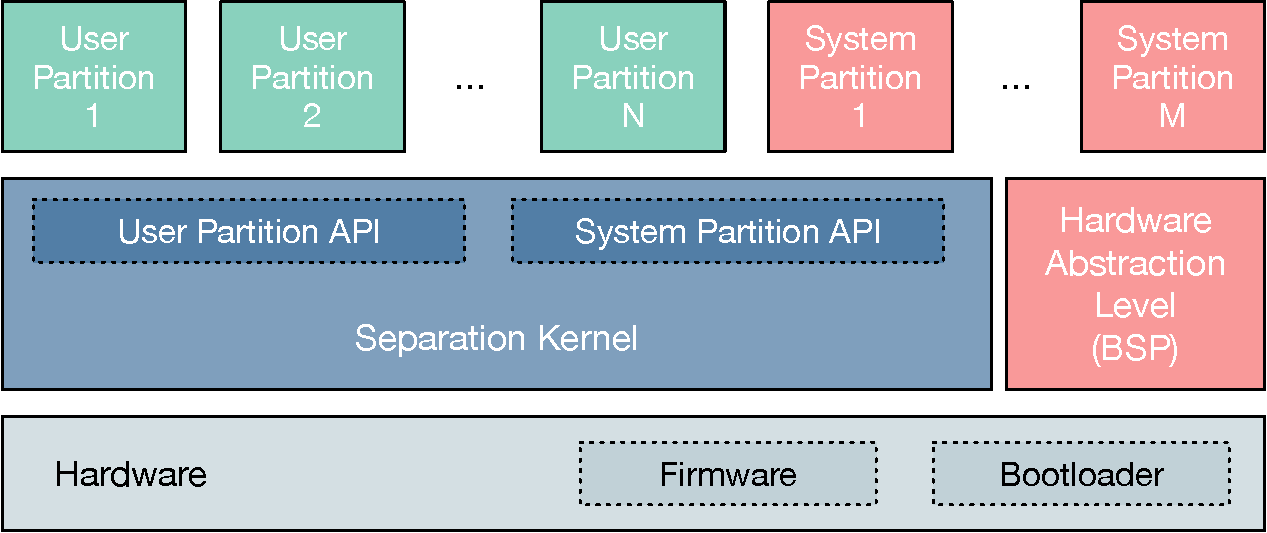
\includegraphics[width=0.7\textwidth]{SeparationKernel}
\caption{Typical Separation Kernel Architecture}
\label{fig:separationkernel}
\end{figure}
A partition is a logic unit maintained by the separation kernel, and each of them is separated from the other. For each partition, the separation kernel provides resources such as physical memory space, I/O memory space, CPUs, and so on (spatial separation). Moreover, separation kernels are typically implemented using time-triggered schedulers and assigning each partition a dedicated time slot in a cycle to provide time separation. Usually two type of partitions are supported: \emph{User Partitions} and \emph{System Partitions}. The partitions are identified configured by the system designer, which is a trusted person. The content of a user partition does not need to be approved by the designer and can be arbitrary, even malicious \cite{mils}, whereas a system partition contains applications and data supplied and approved by the designer. All partitions use the API (Application Program Interface) provided by the separation kernel to interact with it. Since partition are spatially isolated they cannot communicate each other, through the kernel API, they can communicate under the supervision of the kernel. This communication occurs via communication object that is statically configured by the designer. The separation kernel also provides the \emph{Hardware Abstraction Level} called \emph{Board Support Package} (BSP). It contains a set of drivers for specific hardware components, and it is approved by the designer. Since it provides an abstraction of the underlying hardware, an onboard support package can be exchanged without changing the content of any partition.

\paragraph{} Separation kernels are gaining importance thanks to the increasing needs of adoption of multi-core embedded systems.


%********************************** % Section **************************************
\section{Multi-core embedded systems}
The traditional approaches to provide more processing bandwidth were to increase the CPU clock frequency, increase the instruction level parallelism through instruction pipelines, increase the cache size and number of cache levels and so on. With today's technology, this approach is no longer sustainable. Increasing CPU frequency causes excessive power consumption and thermal dissipation loss and raises more and more problems due to internal chip design. Parallelization has become a key solution for this problem. For this reason multi-core platforms have the potential to meet these requirements by offering greater computational capabilities and advantages in size, weight, and power (SWaP). 

\paragraph{} However, in a multicore system different cores share hardware resources such as caches and central memory, which were developed focusing on maximizing the overall performance, but when placed in the safety-critical context introduce challenges to predictability.
\par Safety-critical multi-core CPS are still not fully embraced by industry for safety critical applications. For example, aerospace systems are subject to costly and time-consuming certification processes, which require a predictable behavior under fault-free and certain hazardous conditions, hard to prove in multi-core platforms. Albeit the industry is moving towards higher exploitation of commercial-off-the-shelf (COTS) devices to reduce development cost\cite{mulcors}, as well as exploiting the low SWaP characteristics of multi-core, despite the fact that the use of such boards is challenging for certification.

\paragraph{} The introduction of COTS multi-core processors is by motivated several aspects:
\begin{itemize}
\item Provide a long-term answer to the increasing demand of processing power.
\begin{itemize}
\item Increased performance: better exploitation of the thread parallelism
\item Increased integration: Less equipment to perform the same functionality or same equipment to
host more functionality
\item Reduce environmental footprint: Fewer embedded equipment, less power consumption, less dissipation compared to
the single core equivalent
\end{itemize}
\item Anticipate mass market obsolescence of single-core processors.
\item Be able to "simplify” the overall system architecture (for example a partitioned architecture can avoid Ethernet communication).
\end{itemize}

\paragraph{} The barrier to the adoption of the multi-core technology is its complexity of the certification. For the certification process it is important to ensure the \emph{Execution Integrity} of its software components. That means it will be correctly executed in a nominal situation, and the system state will be predictable in non-nominal situations (internal faults). Moreover, it must be possible to perform a \emph{WCET analysis} (Worst Case Execution Time) of the embedded software. Timing information is tightly coupled with both software and hardware architecture since they introduce \emph{interferences} between parallel applications that are reflected in timing delays. In COTS this analysis become even more difficult because of the lack of documentation on the system design.

\subsection{Hardware interference channels} 
Applications running on different cores of a multi-core processor are not executing independently from each other. Even if there is no explicit data or control flow between these applications, a coupling exists at platform level since they are implicitly sharing platform resources. A platform property which may cause interference between independent applications is called a hardware interference channel. The analysis of hardware interference channels requires a deep understanding of the platform architecture including the CPU internals.
\par In this work, we consider only commercial multi-core platforms rather than designing new architectures. Therefore we assume that the platform implements the Unified Memory Model, which means that all cores share the same physical address space. Figure \ref{fig:unifiedmemorymodel} depict a typical architecture of such platform.

\begin{figure}[htbp] 
\centering    
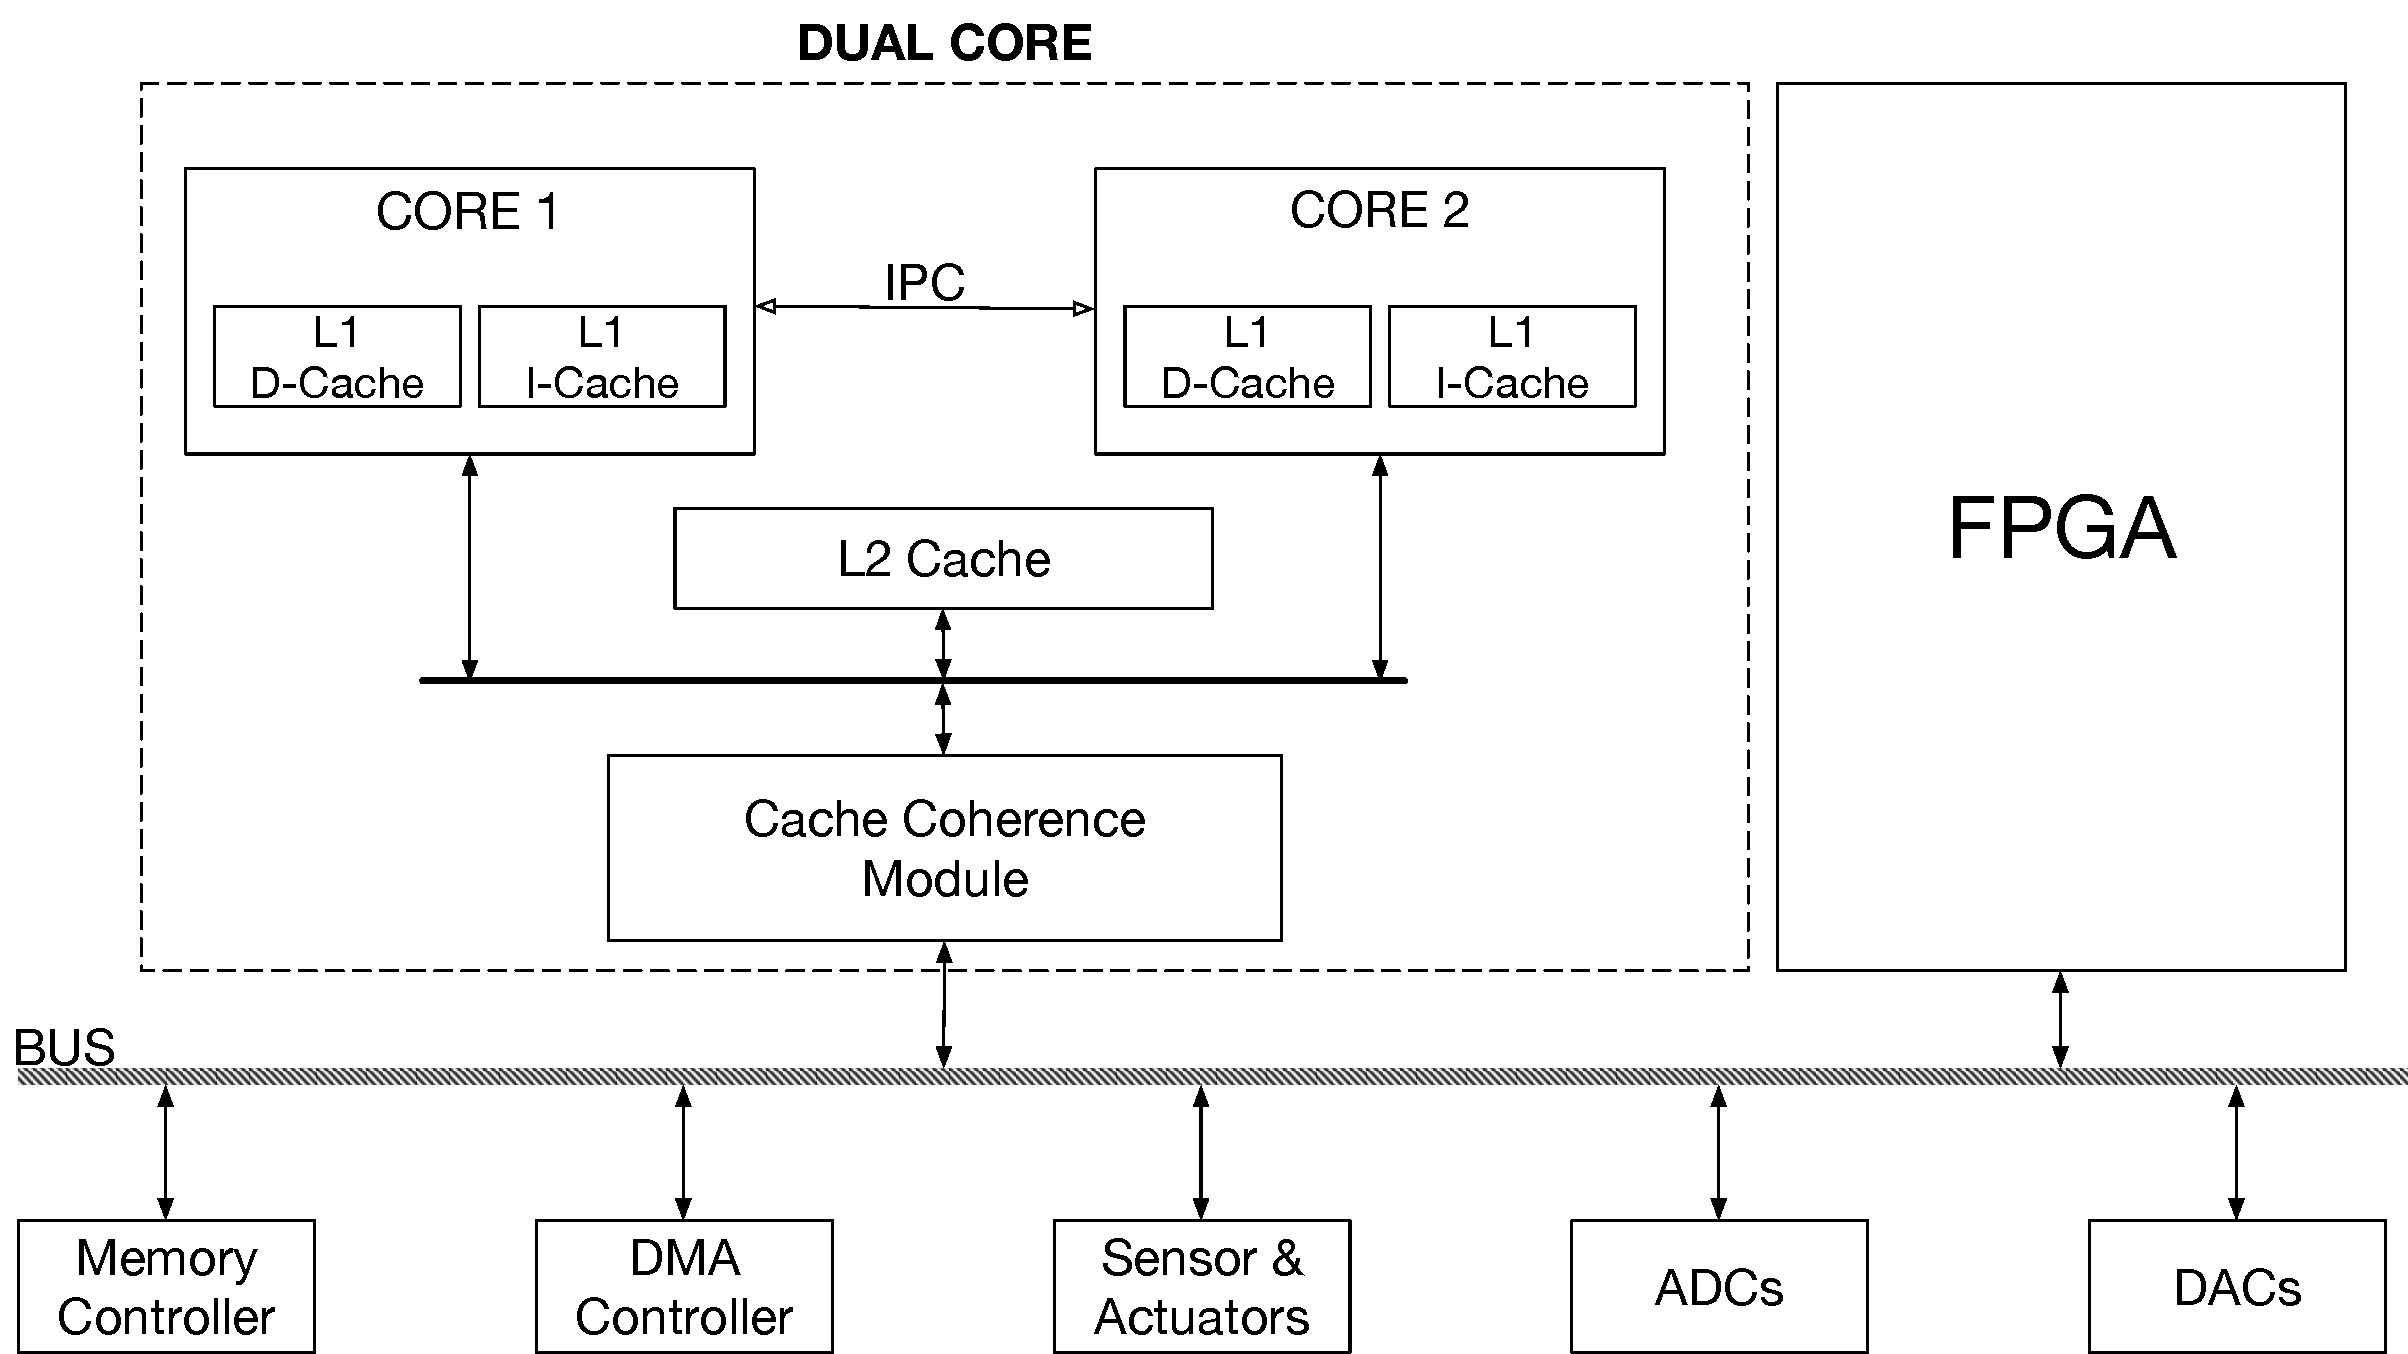
\includegraphics[width=1.0\textwidth]{UnifiedMemoryModel}
\caption{Unified Memory Model Architecture}
\label{fig:unifiedmemorymodel}
\end{figure}

\subsubsection{Caches}
While two different cores can execute independently as long as they are not using shared resources, caches may introduce cross-CPU interference trough \emph{Cache Coherency} and \emph{Cache Sharing}. The L1 cache is typically divided into data and instruction cache while all other levels store data as well as instructions. Most multi-core processors have a dedicated L1 data and instruction cache for each core while other levels might be shared or not depending on the architecture. Shared caches are an essential cause of interference in a multi-core processor. If data used by tasks are small enough to fit inside the private cache of the processor no performance loss occur, if it is not the case, data are replaced according to some \emph{cache replacement algorithm} on demand of executing tasks among all cores. Therefore tasks start to experience long delays due to the recurring access to memory.

%\subsubsection{Cache Coherency}
\paragraph{} Another important aspect related to the use of caches is the consistency of local caches connected to a shared resource. Cache coherency is crucial in multi-core systems because: if one of the local caches of a core contains a reference to a physical resource, and the cached value is more recent than the value stored in the physical resource itself then any read access from any core must provide the value cached. In multi-core processors, cache coherency is solved by utilizing the core communication bus. So this mechanism determines how the memory system transfers data between processors, caches, and memory.

\subsubsection{Interconnect}
Multi-core processors are often part of a System on Chip (SoC) where the cores are packed together with peripherals such as external memory, serial I/O and Ethernet. To handle all requests to the shared peripherals, an \emph{interconnect} is implemented to arbitrate the requests. It is the key point where all the accesses are performed. Indeed, the interconnect has been built to sustain a higher bandwidth to serve all cores efficiently. Usually, a significant source of performance degradation is the concurrent access to shared Bus and shared I/O device such as the graphical device, the GPIO (General Purpose Input Output) or the network interface. If a device can handle one request at a time, it may block the second request for hundreds of microseconds, or even worst to milliseconds. Moreover, shared devices can also rise Interrupts. On multi-core platforms, a hardware interrupt is typically routed to one core. If multiple devices are attached to one interrupt line and the devices are not served by the same core, the core which receives the interrupt must pass this interrupt also to the other core(s). All these factors worsen the determinism of the systems and WCET analysis. Indeed, the execution time of software on one core depends on software executed on the other cores because of potential inter-core conflicts. The internal workings of the interconnect and how it prioritizes the requests are often part of the manufacturer's intellectual property, and they heavily impact on the amount and the duration of interferences. It may be difficult to determine an upper bound on their impact whatever the concurrent software even with full information on the design.
\par Characterizing the behavior of the interconnect in every possible situation in multi-core COTS is technically difficult. To overcome this problem the \emph{Interconnect Usage Domain} can be defined as a set of constraints restricting the accesses to the interconnect. The usage domains give the possibility to treat the interconnect as black-box. The objective is to reach an acceptable characterization of the interconnect behavior to enable further analyses even with poor documentation on the behavior.

\paragraph{} How these interference channels impact of the concurrent application also depends on the software architecture.

%\subsection{Software Interference}
%Obviously tasks interfere with each other due to access to shared I/O devices. However, can be noticed that the Operating Systems can be source of interference too. It must provide an execution environment for the hosted applications which on the one hand hides the platform characteristics from the hosted applications and on the other hand strictly controls the use of platform resources for all applications. Usually the operating system uses some additional software components called Board Support Package (BSP), it is the implementation of specific support code for a given board that conforms to a given operating system.   
%\par The diversity of Multi-Core System on Chip (MPSoC) architecture leads to additional effort (and issues) during certification since the operating systems, the BSP and the code on top of them, must be certified by authorities. 

\subsection{Parallelism basic concepts}
There are several types of parallelism used in multi-core programming, we can fist distinguish between \emph{Task Level Parallelism}, \emph{Data Level Parallelism}, and \emph{Instruction Level Parallelism} \cite{computerarchitecture}. Instruction level parallelism refer to overlapping the execution of instructions to improve performance. There are two largely separable approaches to exploiting this parallelism approach: \begin{enumerate*} \item an approach that relies on hardware to discover and exploit the parallelism dynamically, and \item an approach that relies on software technology to find parallelism statically at compile time.\end{enumerate*} Data level parallelism focuses on distributing the data across different cores, which operate on the data in parallel. It is commonly applied on regular data structures like arrays and matrices by working on each element in parallel. Finally, Task level parallelism focuses on distributing tasks (functional units) across cores. While Instruction and Data Level Parallelism are highly exploitable in FPGA and GPU, in this work we focus only on Task Level Parallelism.
\paragraph{} At system level, Task Level Parallelism can distinguished into two other classification: \emph{Asymmetric Multiprocessing} (AMP) and \emph{Symmetric Multiprocessing} (SMP).

\subsubsection{Asymmetric Multiprocessing}
In this approach each core runs its own single-core aware application (a partition) as in figure \ref{fig:AMP}. Therefore, scheduling inside a partition is sequential. The advantages of using this programming approach are:
\begin{itemize}
\item applications do not need to be multi-core aware; this simplifies the design.
\item reduced need to mutual exclusion.
\item interferences are mainly caused by shared caches, memory, I/O buses and concurrent access to shared devices.
\end{itemize}
The disadvantages are:
\begin{itemize}
\item all applications must be certified to the highest assurance level since they have full access to the processor;
\item it can be hard to identify different single-core aware, independent applications; this can limit the use of cores to few of them;
\item synchronization among applications running on different cores is more complex.
\end{itemize}

\begin{figure}[htbp]
  \centering
  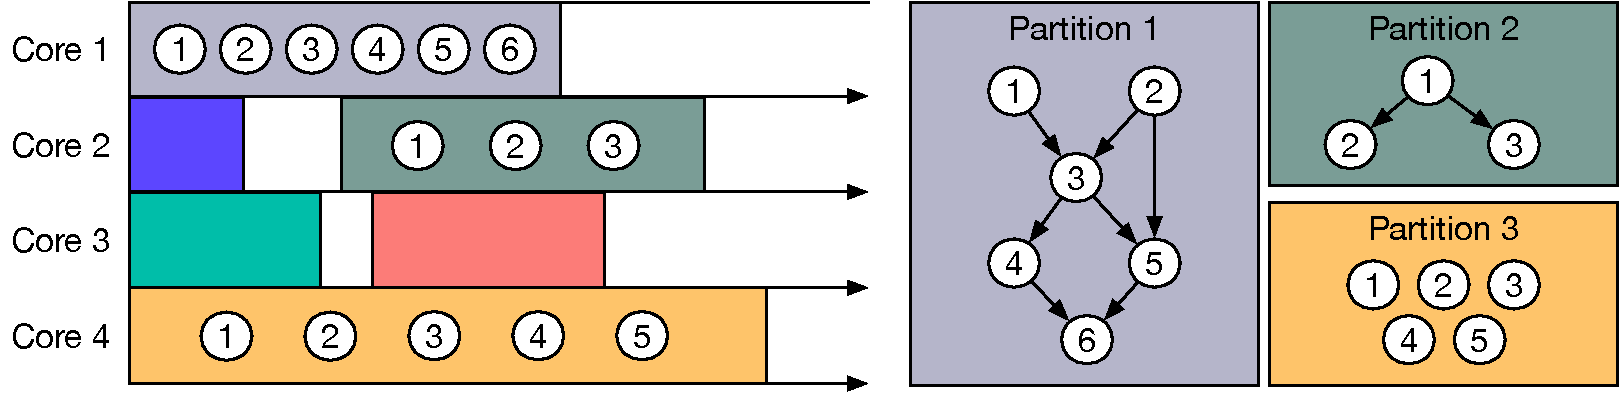
\includegraphics[width=0.7\textwidth]{AMP}
  \caption{Example of Asymmetric Multiprocessing}
  \label{fig:AMP}
\end{figure}

\subsubsection{Symmetric Multiprocessing}
In this approach each application has access of all cores. Threads inside the partition run concurrently and the Operating System typically controls cores and platform resources as shown in figure \ref{fig:SMP}. The advantages of this approach are:
\begin{itemize}
\item More flexibility is allowed and better load balancing can be achieved.
\item There is only one system component responsible for the partitioning.
\item Different safety-levels are allowed in the system (mixed-critical systems).
\item Application can still be completely isolated by the other, e.g. by disabling concurrent execution.
\item Inter-process conflicts does not impact time and space partitioning as they occur inside the same partition.
\end{itemize}
\par The disadvantages comes from this additional system level software components:
\begin{itemize}
\item System level components responsible for the partitioning are complex and must be certified with the highest level of insurance.
\item Synchronization effort can be higher.
\item Due to the shared system software layer, an implicit coupling of unrelated threads cannot be completely avoided.
\end{itemize}
A careful design can limit the impact of these drawbacks. 

\begin{figure}[htbp]
  \centering
  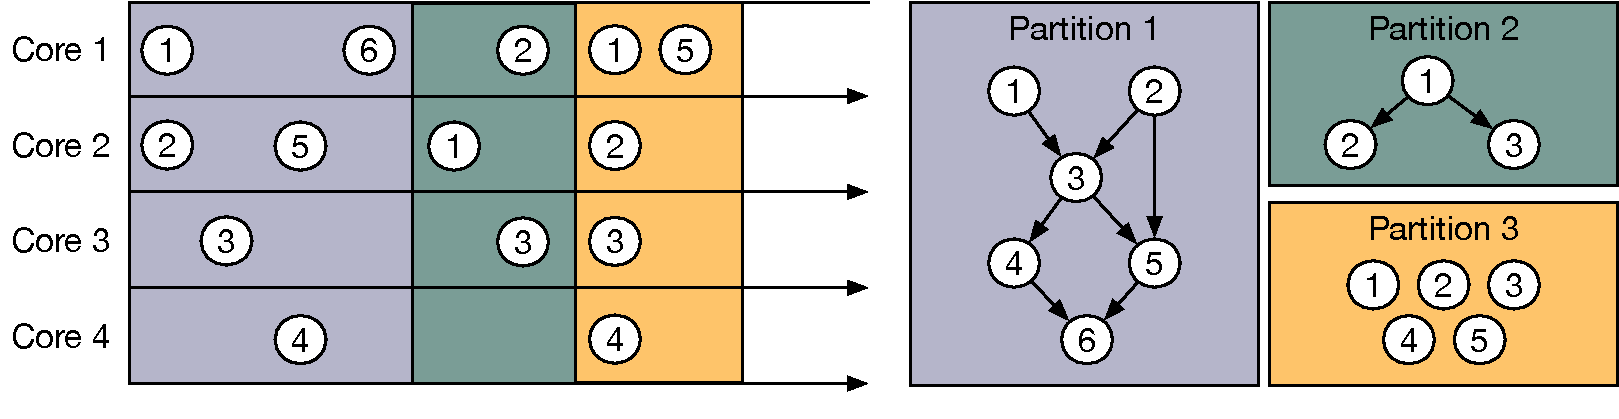
\includegraphics[width=0.7\textwidth]{SMP}
  \caption{Example of Symmetric Multiprocessing}
  \label{fig:SMP}
\end{figure}

\subsubsection{Selected approach}
The asymmetrical approach presents some difficulties in the demonstration of robust partitioning. It is interesting for very specialized applications, for example where, in a dual-core platform, one core is completely dedicated to I/O processing and the other core runs the application software. On the other hand, the symmetric approach needs to be considered to take benefit from platform. All its drawbacks  are manageable if the systems runs under control of the (trusted) operating systems and the design take into account all the possible issues. Moreover we assume that future embedded systems have to host, besides the critical applications, an increasing number applications with high performance requirements but lower criticality.

\paragraph{} Implementing a mechanism to isolate different application inside a multi-core platform is crucial. A virtualization layer hosting several virtual machines can provide this service.

%********************************** % Section  **************************************
\section{Virtualization in Embedded Systems}
The main concept for the design of a mixed-critical system is, first and foremost, the demonstration of sufficient independence among software components. System virtualization, which is the abstraction and management of system resources, facilitate the integration of mixed-criticality systems \cite{multipartes}. This approach results in independent virtual machines that are fully contained in an execution environment that can not affect the remaining system. 

\subsection{Overview}
Platform virtualization refers to the creation of \emph{Virtual Machines} (VMs), also called guest OS, running on the physical machine and managed by a \emph{hypervisor}. Virtualization technology enables concurrent execution of multiple VMs on the same hardware (single or multi-core) processor. Virtualization technology has been widely applied in the enterprise and cloud computing field, however, in recent years, it has been increasingly deployed in the embedded systems domain. Virtualization for embedded systems must address real-time behavior, safety, and security such that it offers protection against external attacks and unintended
interactions between the critical and non-critical components of the system. The hypervisor provides an isolation mechanism that can encapsulate an entire OS and applications into a Virtual Machine (VM).

\subsection{Hypervisor types}
In 1974 Gerald J. Popek and Robert P. Goldberg \cite{popek1974formal} classified hypervisors in two categories:
\begin{itemize}
\item \emph{Level II hypervisor} is software layer that runs on top of a General Purpose Operating System (GPOS) \cite{Kleidermacher2013} (fig. \ref{fig:HypervisorL2}). It takes advantage of the underlying Operating System services and hardware abstraction to enable the creation of virtual machines. However, the security of type II hypervisors is as robust as the host GPOS. Therefore, the hypervisor can be subverted by one of the security gaps in the host GPOS, thereby corrupting the entire system. Additionally, the host OS layer increases system complexity and overall code size, which is a major factor for resource-constrained embedded systems. As a result, type II hypervisors are not suited for most embedded systems.
\item \emph{Level I hypervisor} is software layer that runs directly on the hardware platform (bare-metal) (fig. \ref{fig:HypervisorL1}. This approach avoids the complexity and inefficiency of GPOS, and can achieve a higher level of isolation for safety and security critical applications \cite{Kleidermacher2013}.
\end{itemize}

\begin{figure}
  \begin{subfigure}{0.5\textwidth}
    \centering
    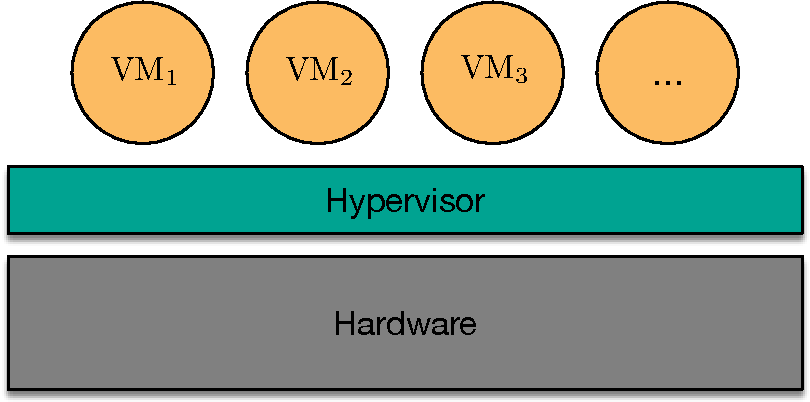
\includegraphics[width=.9\textwidth]{HypervisorL1}
    \caption{Type I}
    \label{fig:HypervisorL1}
  \end{subfigure}%
  \begin{subfigure}{0.5\textwidth}
    \begin{subfigure}{\textwidth}
      \centering
      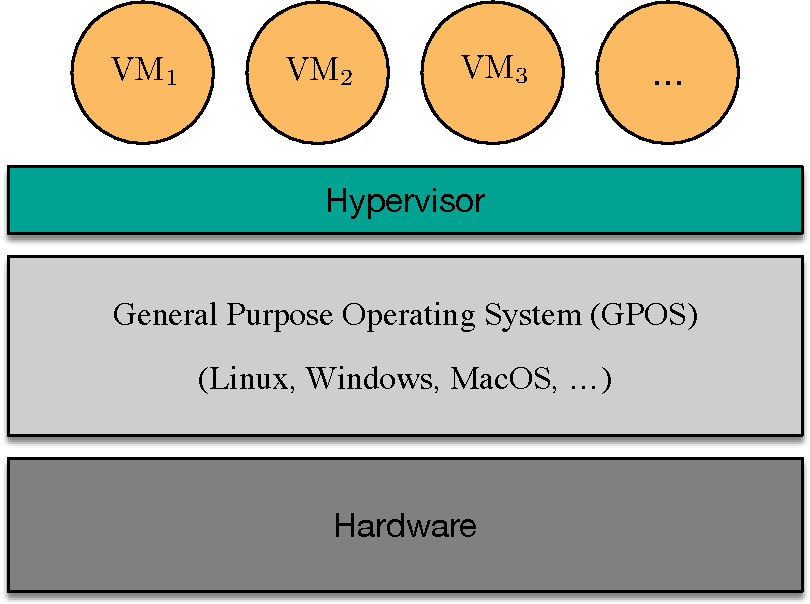
\includegraphics[width=.8\textwidth]{HypervisorL2}
      \caption{Type II}
      \label{fig:HypervisorL2}
    \end{subfigure}
  \end{subfigure}
  \caption{Hypervisor Types}
  \label{fig:interactions}
\end{figure}
The selected operating system, PikeOS, is a Level I hypervisor. It provides safe and security services through virtualization.

\subsection{Virtualization Approaches}
Virtualizing an operating systems requires placing a virtualization layer under the operating system to create and manage the virtual machines. As clarified below, virtualization is provided mainly in two ways \cite{practicalmicrokernel}:
\begin{itemize}
\item \emph{Full/Native Virtualization}. With this technique, guest operating systems are unmodified and unaware of the virtualization environment. Each virtual machine is provided with all services of the physical system (e.g. virtual BIOS, virtual devices, and virtual memory). Full virtualization usually employs binary translation techniques to trap-and-emulate non-virtualizable and sensitive system instructions or hardware assistance \cite{vmwarevirtualization}. However, the computational complexity of this technique results in an unacceptable performance level for embedded systems \cite{Kleidermacher2013}.
\item \emph{Para-virtualization}. Unlike full virtualization, in para-virtualization, guest operating systems are modified to improve the performance of the hypervisor. These modifications are applied specifically to the guest OS kernel to replace non-virtualizable instructions and critical kernel operations with hypercalls that can request services directly from the hypervisor. These services represent system calls that are part of the OS kernel, and they execute with the highest privilege level in the system. Consequently, the hypervisor is the only software component to be executed in privileged mode. Para-virtualization overcomes the issues of full virtualization, and it is the only viable solution for embedded platforms that do not provide any hardware virtualization support\cite{Kleidermacher2013}.
\end{itemize}

\subsection{Microkernel-Based Hypervisor}
In order to increase the robustness of the hypervisor, its size should be as small as possible. Microkernel-based hypervisors represent a thin software layer that runs as bare-metal in the highest privileged mode. It can provide strong isolation among guest operating systems. This approach implements virtualization as a service on top of the trusted microkernel wich is the near-minimum amount of software that implements the needed mechanisms to implement an operating system. Therefore, each separate instance is as robust as the guest environment itself. Consequently, since the code size of the hypervisor is small, it is easier to verify and validate. Authors from Lockheed Martin \cite{LockheedMartinVMIMA} presented a study towards applying a Microkernel-Based Hypervisor architecture to enable virtualization for a representative set of avionics applications requiring multiple OS environments and mixed-critical application. 

%\subsection{Requirements for mixed-criticality}
%The main concept for the design of a mixed-critical system is, first and foremost, the demonstration of sufficient independence. Common mechanisms are: 
%\begin{itemize}
%\item kernels and schedulers that guarantee resource and time isolation; separation kernels are the most notable example.
%\item monitors to detect timing faults (and eventually control them), and the scheduling schemes for guaranteeing controllability in the presence of faults.
%\end{itemize}
%\par A separation kernel is an operating system that enforces spatial and temporal separation among functionalities or partitions that are managed by it. One example that can be found in the state of the art is the commercial Hypervisor/OS called pikeOS from SysGO, it implements the avionic ARINC 653 standard, consisting of a separation microkernel that provides paravirtualization to real-time operating system for running partitions. 
%\par Monitors can be used to prevent the propagation of failures and reduce the criticality of but they introduce overhead and further certification issues. PikeOS also provides mechanism for implementing monitors and different scheduling schemes.

\subsection{Available Solutions}
Many hypervisor solutions are available as either open-source or commercial products. For example Xen hypervisor has recently been ported to the Xilinx Zynq Multi-Processor System-on-Chip (MPSoC) devices \cite{xenZynq}. Xen Zynq Distribution is released under the GNU General Purpose License 2 (GPL2) but it is not designed for mixed-critical applications. On the other hand there are several commercial RTOS products that comply with the ARINC 653 standard \cite{embeddedvmstate}, e.g. LynuxWorks LynxOS-178 \cite{LynxOS}, Green Hills INTEGRITY-178B \cite{INTEGRITY178B}, Wind River VxWorks 653 \cite{VxWorks}, Real- Time Systems GmbH Hypervisor \cite{RTGmbH}, Tenasys eVM for Windows \cite{eVM}, National Instruments Real-Time Hyper Hypervisor \cite{NIHypervisor}, Open Synergy COQOS \cite{COQOS}, Enea Hypervisor \cite{EneaHypervisor} etc. 

\paragraph{} Even though the offer is quite big, in this thesis we focus only on PikeOS \cite{PikeOS} from SysGO AG. It is a microkernel-based Type one hypervisor certified for the most common standards (e.g. Do-178C, ARINC-653, ISO 26262 etc.) and has been designed for functional safety and Security requirements which makes it a suitable choice for our applications.

%********************************** % Section  **************************************
\section{Model Based design}

Applications are evolving to cover more and more complex functionalities. The increase in complexity is leading to an increase in the required throughput, and it is becoming a challenge for software developers. Model-based Design (MDB) appears as an excellent solution to cope with this complexity increase.
\par Model-Based Design is a model-centric approach to system development that enables system-level simulation, automatic code generation, and continuous test and verification. Rather than relying on physical prototypes (that can be very expensive) and textual specifications, Model-Based Design uses a model throughout development. The model includes every component relevant to system behavior—algorithms, control logic, physical components, and intellectual property (IP). MDB is being adopted in all areas of engineering; moreover, certification has matured considerably in the last decade attracting considerable interest from companies; recent studies \cite{mbdaerospaceverification} have shown that the application of model-based certification and formal verification can be a practical and cost-effective solution against certification requirements.
\par Examples of available commercial tools are Simulink\textregistered \cite{Simulink}, SCADE Suite\textregistered \cite{Scade}, LabVIEW\textregistered \cite{Labview} and SystemModeler\textregistered \cite{Modeler}. Open source and research tools include Scicos \cite{Scicos} and Ptolemy\cite{Ptolemy}. In this work we use Simulink which is the \emph{de-facto standard} and provides mature tools for design, simulation, and code generation.

\begin{figure}[htbp]
  \centering
  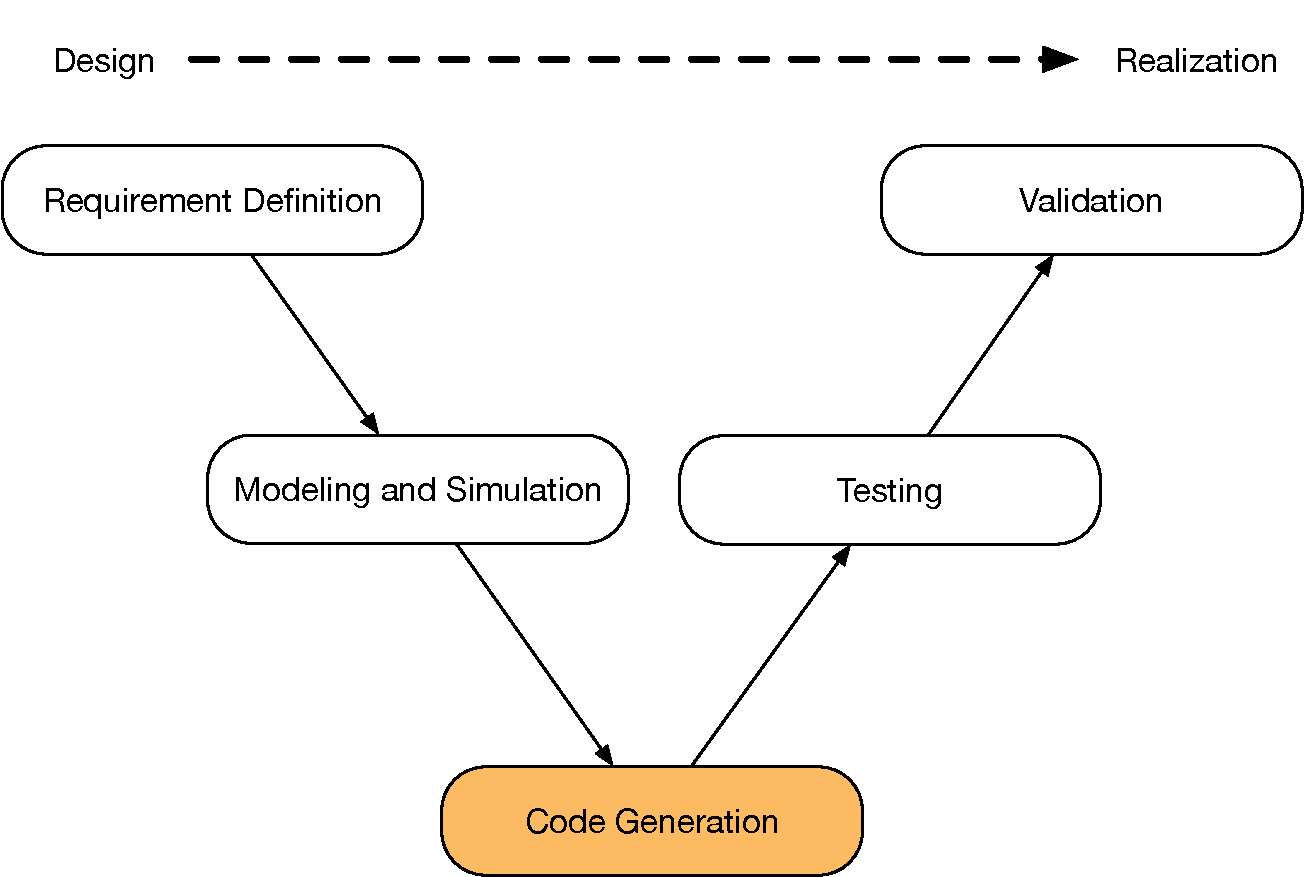
\includegraphics[width=0.7\textwidth]{MBDflowchart}
  \caption{Model-Based Design Flow Chart}
  \label{fig:mbdflowchart}
\end{figure}

\paragraph{} The model includes every component relevant to system behavior-algorithms, control logic, physical components and intellectual property (IP). This make MBD the perfect candidate for a complete work-flow that goes from the system development, verification, validation and deployment. A typical design flow in MDB is shown in figure \ref{fig:mbdflowchart}. The traditional embedded system development process follows the standard \emph{V-shaped} lifecycle. V-cycle splits the product development process into a design and an integration phase. The Code Generation step is the turning point of the process. This work focus on this step. 

%********************************** % Section  **************************************
\section{EMC\textsuperscript{2}}
This work fits inside the European EMC\textsuperscript{2} - "Embedded Multi-Core Systems for Mixed Criticality applications in dynamic and changeable real-time environments" project \cite{emc2artemis}. The objective of the project is to foster changes through an innovative and sustainable service-oriented architecture approach for mixed-criticality applications; the project bundles the power of 98 partners from 19 European Countries and 100 millions of euro in budget.

\paragraph{} Within the EMC\textsuperscript{2} project the objective was to demonstrate the possibility of using a Model-Based Design approach to assist the design and the implementation of mix-critical applications running in multi-core platforms. For that purpose, we selected a typical aerospace use case: motor drive control. This is a widely known application that is used for example in the control of the actuators for the primary and secondary flight control. The platform selected to implement this use case was the Xilinx ZedBoard\texttrademark \cite{zedboard} based on the Xilinx Zynq\textregistered-7000 All Programmable System-on-Chip (SoC). The board is equipped with dual-core ARM\textregistered Cortex-A9 processors and an Artix-7 FPGA which adds more complexity to the design and more flexibility. For the motor control we used the \emph{FMCMOTCON2} \cite{FMCMOTCON2} evaluation kit from Analog Devices (figure \ref{fig:fmcmotcon} which provide a complete motor drive system including a stepper motor, a control board, a low voltage drive board and a Dynamometer drive system.

\begin{figure}[htbp]
  \centering
  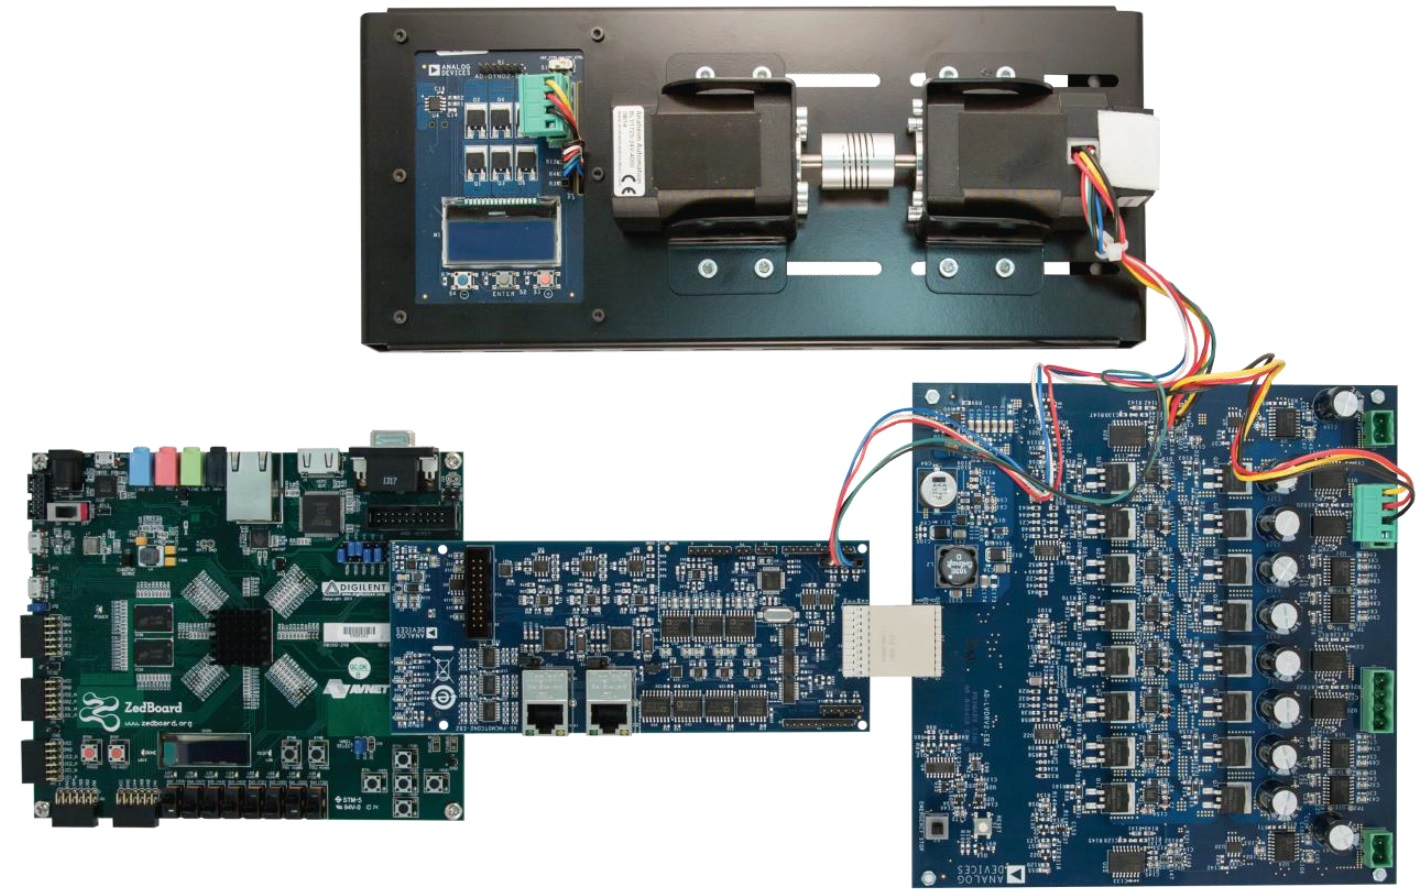
\includegraphics[width=0.9\textwidth]{FMCMOTCON2}
  \caption{Analog Devices FMCMOTCON2 Evaluation Kit}
  \label{fig:fmcmotcon}
\end{figure}

%********************************** % Section  **************************************
%\section{Goal}
%This work presents a model-based approach for automatic code generation for mixed-criticality, multicore, embedded application using an Hypervisor operative system; mainly focusing on aerospace use-cases.
%Our work aims to exploit the multicore platform advantages as much as possible while ensuring an acceptable level of safety among the different mixed critical tasks composing the systems, mainly from aerospace use-cases.

%!TEX root = ../thesis.tex

\chapter{Frameworks and tools}

\ifpdf
    \graphicspath{{Chapters/Figs/Raster/}{Chapters/Figs/PDF/}{Chapters/Figs/}}
\else
    \graphicspath{{Chapters/Figs/Vector/}{Chapters/Figs/}}
\fi


%********************************** % Section  **************************************
\section{PikeOS}
A trusted Operating System, capable of providing isolation among partitions is crucial for mixed-criticality systems. PikeOS \cite{PikeOS} is a commercial operating system from SYSGO AG, designed in early 2002 to address the needs of a kernel targeting safety and security applications. It uses a separation micro-kernel architecture and provides a hypervisor model at its core. Moreover, PikeOS hypervisor has been certified for all relevant certification standards including DO-178C, IEC 61508, EN 50128, EN 62304, and ISO 26262 coming from the fields of Aerospace/Defense, Automotive, Transportation and Industry/IoT.
\par The micro-kernel architecture allows the OS to be used in resource constrained devices like embedded systems. It supports single and multi-core processor architectures with both models: AMP (Asymmetric Multi-Processing) and SMP (Symmetric Multi-Processing).

\paragraph{}PikeOS includes \emph{CODEO}, an Eclipse-based IDE that provides several functionalities such as guided configuration, compilers, assemblers, remote debugging, application deployment, target monitoring, and timing analyses.

\subsection{Hypervisor general overview}
The PikeOS Hypervisor offers a performance optimized para-virtualization, meaning that the OS presents a software interface to virtual machines that are aware of the virtualization level.

\paragraph{} The PikeOS Microkernel consists of a generic part (CPU architecture dependent) called \emph{Architecture Support Package} (ASP) and a platform dependent part called \emph{Platform Support Package} (PSP): together they form the \emph{Board Support Package} (figure \ref{fig:pikeosarch}). 
The PikeOS Microkernel (with the ASP) is the only component that runs with supervisor privileges. It provides:
\begin{itemize}
\item Hardware abstraction
\item Spatial and temporal separation among partition
\item Communication primitives
\end{itemize}
The \emph{PikeOS System Software} (PSSW) component is the first user space application launched by the PikeOS Microkernel, it performs some initialization and, at run-time, acts as a server providing services like communications, file system access, health monitoring and partition/process management to the applications.

\subsection{Personalities}
In PikeOS guest operating systems, runtime environments or API are called \emph{personalities}. They run on top of the hypervisor in a non-privileged mode as shown in fig \ref{fig:pikeosarch}. Personalities included are:
\begin{itemize}
\item AUTOSAR
\item Android
\item Embedded Linux
\item Native PikeOS
\end{itemize}
Moreover, regarding the runtime environments:
\begin{itemize}
\item Ada
\item AFDX (Avionics Full-Duplex Switched Ethernet)
\item ARINC-653 (Avionics Application Standard Software Interface)
\item Certified POSIX
\item RTEMS (Real-Time Executive for Multiprocessor Systems)
\item Real Time JAVA
\end{itemize}
Other personalities are supported through SYSGO partners.
\par These guests are contained inside a Virtual Machine with their memory space, resources and application set. Applications hosted on one virtual machine run completely independently of those in the others. 

\begin{figure}[htbp] 
\centering    
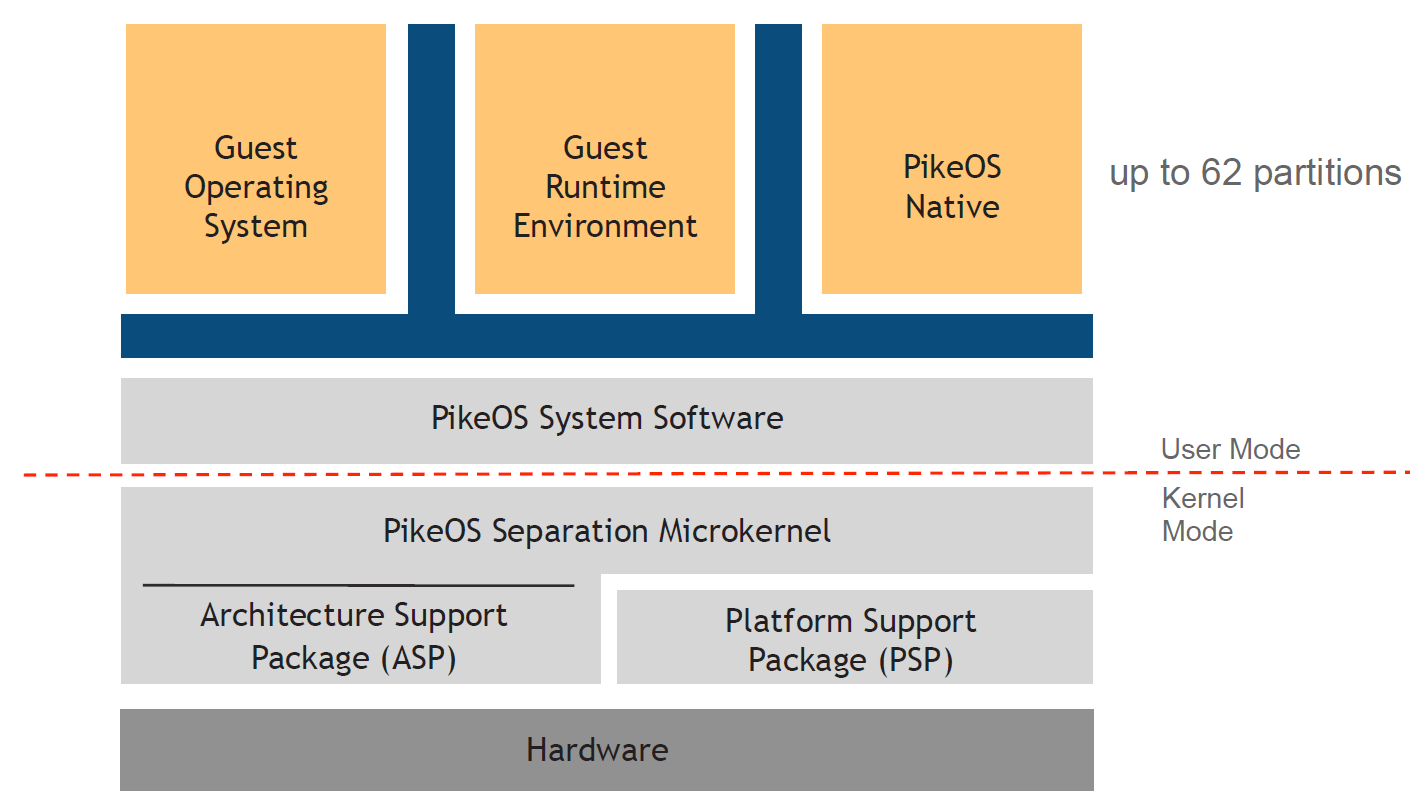
\includegraphics[width=1.0\textwidth]{PikeosArchitecture2}
\caption{PikeOS System Architecture}
\label{fig:pikeosarch}
\end{figure}

%\paragraph{} As an example of the use of guest personalities can be the use of Android, it is is being adopted for infotainment functions because they are a perfect fit for this Operating system. However, its openness and lack of security make it highly hackable, giving a \emph{'way in'} to the critical functions. Utilizing secure separation a designer may choose to host Android in open partition and separate it from the critical functions which are running in another partition. This also provides an evolutionary path whereby partitions can be added while leaving legacy software unchanged. 

\subsection{Resource Partitions}
Resource partitions are one of the basic security mechanisms to support multiple virtual machines on top of PikeOS. They can be thought of as containers within which applications execute. Partitions define the system resources that their applications can use and provide protection domains between different applications. For this reason, PikeOS partitions are also referred to as \emph{resource partitions} (fig.\ref{fig:pikeosExecEntities}). An application running in one partition is completely unaware of applications in other partitions, and cannot access resources to which it does not have explicit access permission. A partition can be stopped, restarted or reloaded with different applications without affecting other partitions. PikeOS supports up to 63 resource partitions. All resource partitions are created by the kernel at boot time.

\begin{figure}[htbp] 
\centering    
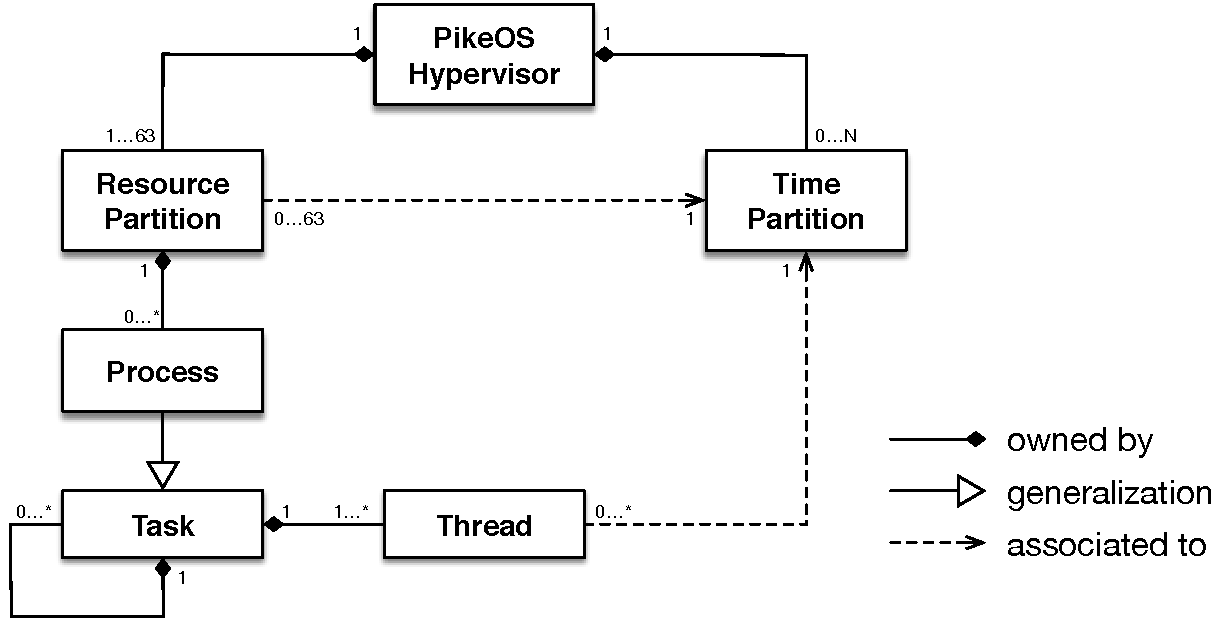
\includegraphics[width=1.0\textwidth]{PikeosExecEntities}
\caption{PikeOS Execution Entities}
\label{fig:pikeosExecEntities}
\end{figure}

\paragraph{} Resource partitioning is enforced by using the MMU to control access to the available resources. To access a resource, each hardware device is somehow represented by a physical address. Thanks to this, resource partitioning can be realized by forcing the MMU to map a certain memory area into a partitions virtual memory space and allow or deny read/write access to this memory space. The configuration of the MMU is done statically at system startup in the PikeOS microkernel and is not modifiable at run-time, also ensuring security. In summary, the separation makes sure that errors occurring in one partition cannot propagate to another partition.

\subsection{Processes and Tasks}
Inside a resource partition we can find different \emph{processes} that, from the kernel point of view, are PikeOS \emph{tasks} (see fig.\ref{fig:pikeosExecEntities}). Each process has its access rights to resources, including CPUs. The set of processors on which task threads can be scheduled, can be specified in the CPU mask attribute. 

\paragraph{} Moreover, each PikeOS task has a set of abilities associated with it, which the kernel uses to verify that the task’s threads have sufficient permissions to use certain kernel services. An ability is said to be enabled if the task is allowed to use the corresponding kernel service, and it is said to be disabled if the task is denied use of that service. Abilities are a task property, so all threads within a task share the same set of abilities.

\subsection{Threads}
Threads are the schedulable entities of a task. Each thread has it execution priority and, again, the affinity mask that express on which processors the thread can be scheduled. A thread may assume one of the following states (fig. \ref{fig:ThreadStates}):
\begin{itemize}
\item \emph{Inactive}. Threads in the INACTIVE state are never scheduled and are not valid targets for communications. When a task is activated, all threads are in the INACTIVE state. Also, a thread delete can put the target thread in this state.
\item \emph{Current}. A thread which owns the CPU is in the state. This thread (the current thread) can either execute user-level code or execute code inside the PikeOS kernel.
\item \emph{Waiting}. A thread is in this state if is waiting for a communication, an event, a resource.
\item \emph{Ready}. A is tread in this state if it is ready to continue its execution. Therefore is eligible to become the current thread.
\item \emph{Stopped}. A thread in this state is never eligible to become the current thread.
\end{itemize}

\begin{figure}[htbp] 
\centering    
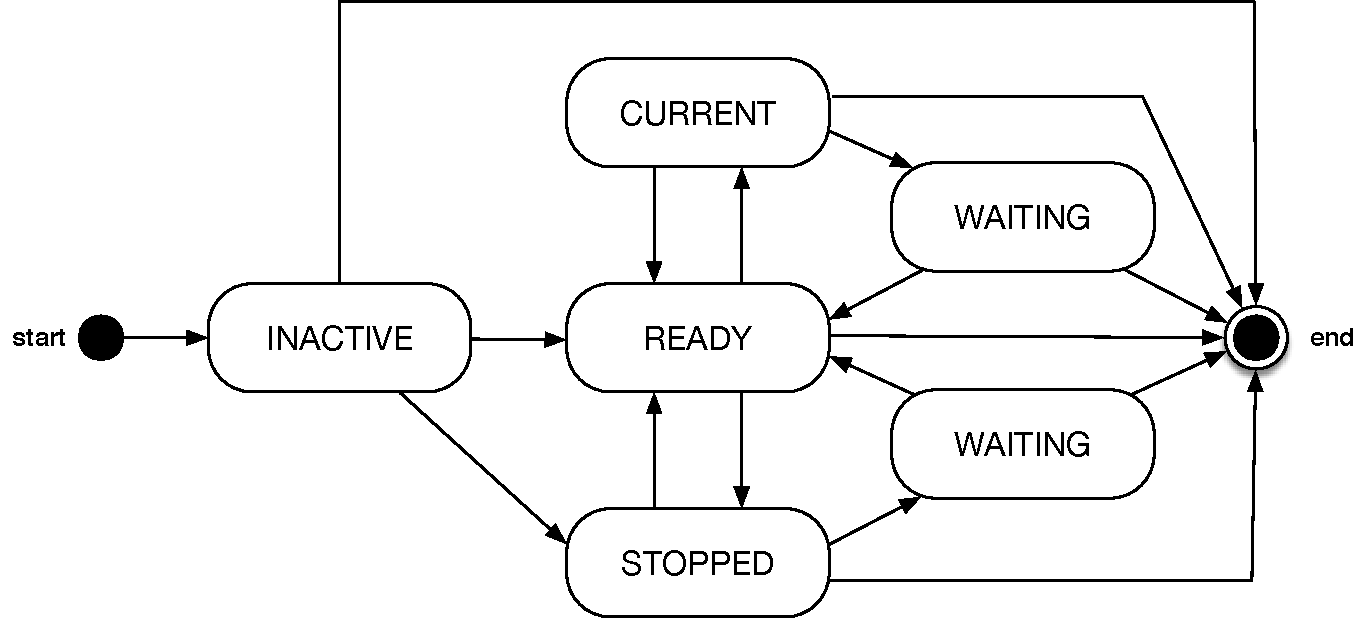
\includegraphics[width=1.0\textwidth]{ThreadStates}
\caption{PikeOS Thread States}
\label{fig:ThreadStates}
\end{figure}

A thread is put into the STOPPED state using p4\_thread\_stop().

\subsection{Time Partitions}
The PikeOS partition scheduler uses a combination of priority-based and time-driven scheduling. 
\par In contrast to the ARINC 653 standard, PikeOS scheduling uses a n-to-one assignment of resource partitions to time-partitions. This means that one or more resource partitions can be assigned to one time-partition. In this work, time partitioning is used to allocate a given amount of CPU time to each resource partition (even though PikeOS allow  a many-to-1 mapping, our approach is fully ARINC 653 compliant). In this case, there is a \emph{one-to-one relationship between time and resource partition}s. This type of configuration is illustrated in figure \ref{fig:TimePartitioning}. Moreover, a PikeOS partition may host more than one task (Process), but in this work, each task is assigned to one and only one resource partition.
\paragraph{} Each Time Partition consists of one or more \emph{Time Windows} representing time intervals allocated to the Time Partition. Each Time Window can be marked as the start of a new period, allowing a static definition of preemption between partitions.

\begin{figure}[htbp] 
\centering    
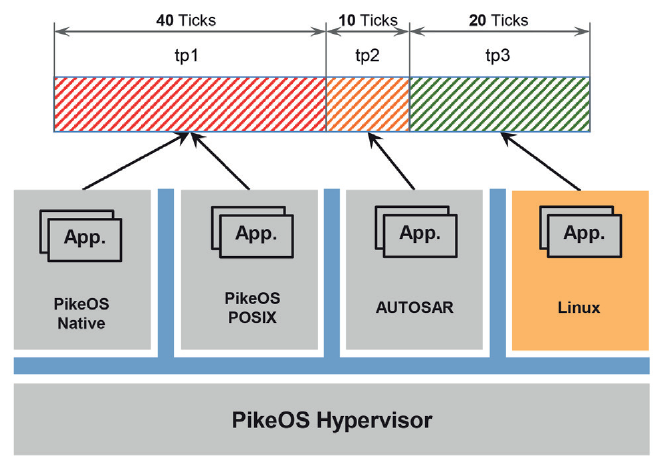
\includegraphics[width=0.8\textwidth]{TimePartitioning}
\caption{PikeOS Time Partitioning}
\label{fig:TimePartitioning}
\end{figure}

\paragraph{}It is worth mentioning that, in contrast to the ARINC 653 standard, there is one special partition that is active at all times. This time partition is referred as the \emph{background partition}\footnote{Background time-partition in parallel to the active
time-partitions is an invention by SYSGO and under active patents.}, \TP{0}, whereas the currently active time-switched partition is called the \emph{foreground partition}, \TP{i} with $i={1,...,N}$.

\subsection{PikeOS Scheduler}\label{sec:P4Scheduler}
Each time partition has its own priority, in addition to that, threads also have a priority attribute. Whenever both the foreground and background partitions have active threads, the thread to be executed is selected according to its priority. Figure \ref{fig:PikeosScheduler} shows the principle of operation: each time partition is represented as a priority-sorted list of FIFO ready queues. Each of them delivers its highest priority ready thread and of these, the highest priority one from either \TP{0} or the currently selected \TP{i} gets chosen for dispatch.

\begin{figure}[htbp] 
\centering    
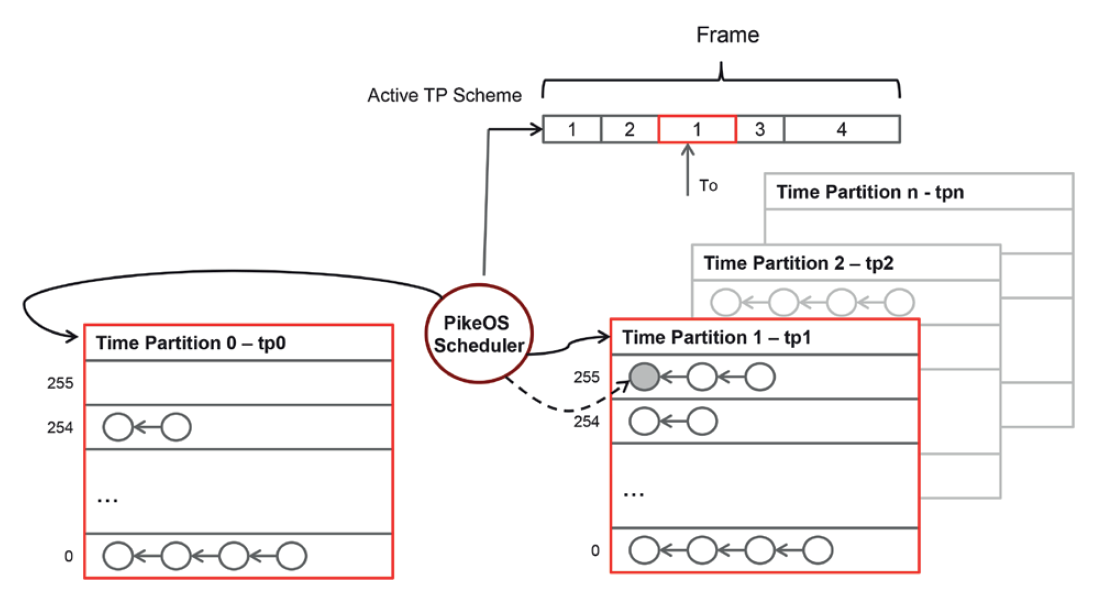
\includegraphics[width=1.0\textwidth]{PikeosScheduler}
\caption{PikeOS Time Partition Scheduler}
\label{fig:PikeosScheduler}
\end{figure}

\paragraph{} Partitions periodically receive guaranteed time slices. But, whenever one partition completes its job prior to having consumed its entire time slice, the unused time automatically falls back to the next lower priority thread in the background time partition. Thus, by running explicitly non-real-time applications with lower priority threads in the background time partition (\TP{i}),  non real-time applications can receive spare computational resources that were assigned to, but not consumed by real-time application in the foreground partition (\TP{i}). This simple approach allows to improve the throughput of safety-critical systems. Figure \ref{fig:PikeosLowTP0}).

\begin{figure}[htbp] 
\centering    
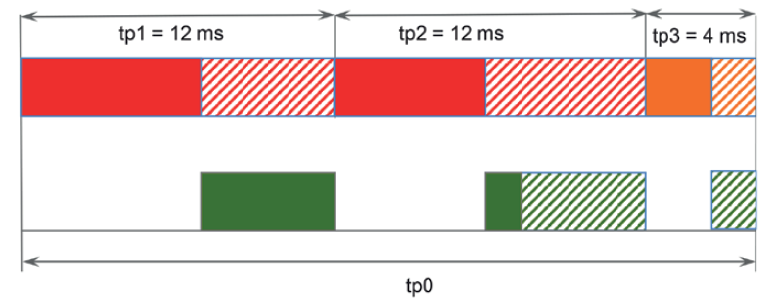
\includegraphics[width=0.7\textwidth]{PikeosLowTP0}
\caption{PikeOS Scheduling with low priority background application}
\label{fig:PikeosLowTP0}
\end{figure}

In a somewhat opposite scenario, it is possible to define threads in the background domain, which can override time partitioning by assigning them a priority above those of the foreground domain threads (fig. \ref{fig:PikeosHighTP0}). 

\begin{figure}[htbp] 
\centering    
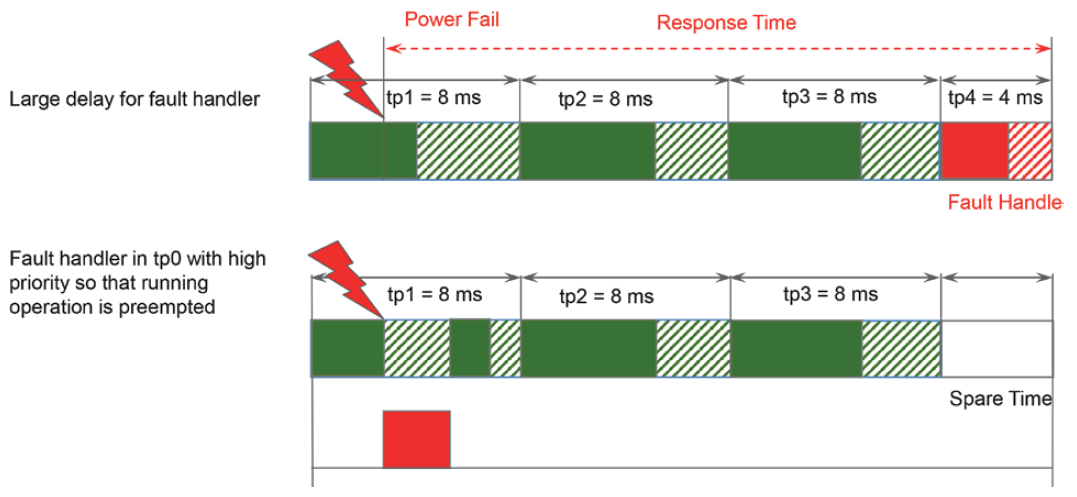
\includegraphics[width=1.0\textwidth]{PikeosHighTP0}
\caption{PikeOS Scheduling with with high priority background application}
\label{fig:PikeosHighTP0}
\end{figure}

\paragraph{}The upper time-diagram in Figure \ref{fig:PikeosHighTP0} has a fault handler, which can be executed in a dedicated time-partition \TP{4}. In case of a failure the response-time of the fault-handler can be high if the error happens right after the fault handler time-partition has ended. By assigning the fault handler to \TP{0}, the handler is starter immediately, as it has the highest priority among all active threads (lower time-diagram of Figure \ref{fig:PikeosHighTP0}). Clearly, such high priority threads must be considered as trusted code from the point of view of the threads that they can preempt.

\paragraph{} PikeOS support the possibility to change, at runtime, the Time Partition schedule. Each schedule is expressed (statically) inside the configuration file, and it is called \emph{scheme}. Schemes allow the system designer to adjust the time partitioning to handle exceptional situations rather than having to design a single time partitioning scheme which will suit all possible scenarios. The following XML code fragment shows a configuration with two schemes named "SCHED\_BOOT" (which is the one loaded at startup) and "SCHED\_POWERFAIL".
% CODE FRAGMENT
\lstinputlisting{Chapters/SrcCode/ScheduleScheme.xml}

\par Where the duration is expressed in \emph{Ticks}. Each Time Windows can be marked as a new period starting point just adding \emph{VM\_SCF\_PERIOD} its flags field.

\paragraph{} The PikeOS hypervisor provides means to invalidate instruction caches and TBLs and to flush the data cache between time partition switches (fig. \ref{fig:PikeosCacheFlush}). This ensures that caches and TLBs are in a defined state when a partition starts its execution. The cache/TLB flush and invalidate operation takes place during the time partition switch, so it will introduce a delay for the partition activation and thus cause a jitter. A possible approach to know the duration \cite{PikeosScheduling} of this delay is to define a small (but big enough) time partition window, which is allocated to an unused time partition ID and to insert this before the time critical application. This eliminates the jitter of the time critical application.

\begin{figure}[htbp] 
\centering    
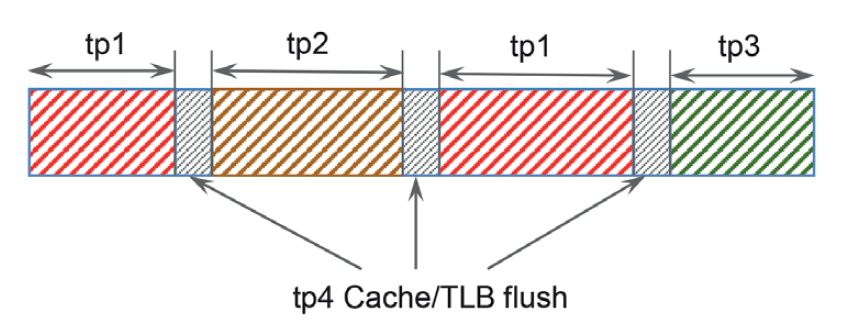
\includegraphics[width=0.8\textwidth]{PikeosCacheFlush}
\caption{PikeOS Cache and TLB Flushing}
\label{fig:PikeosCacheFlush}
\end{figure}

\subsection{Timeouts}
The PikeOS kernel provides a logical timebase for system time and timeouts. The system time value represents the elapsed time since startup. The resolution of the system time is platform- and configuration-dependent.

\par The PikeOS kernel provides different types of timeouts, in this work only \emph{Normal Timeouts} are used. They are timeouts that specifies a point in time with respect to the system time. Each timeout can be absolute or relative: an absolute timeout specifies the timeout as a system time value, while a relative timeout specifies the timeout as a difference relative to the current system time. Valid values are:
\begin{itemize}
\item \verb|P4_TIMEOUT_NULL|
\item \verb|P4_TIMEOUT_INFINITE|
\item numeric values
\end{itemize}

Expired timeouts are evaluated with a minimum frequency corresponding to the period of the system tick. Timeout expiration is checked before every rescheduling decision. A rescheduling is always evaluated when a system tick is processed by the kernel. However, the effective expiration depends on whether a time window of the caller's time partition is active or not. If the caller’s time partition is active, the timeout expires immediately. If no window of the caller’s time partition is active, the timeout does not expire when this time point is reached. The caller remains blocked, and the effective timeout expiration occurs when the caller’s time partition is next activated. In the first case, the thread may be scheduled immediately if it has the highest priority in the system. In the second case, the service call behaves as if the timeout did not expire.

\subsection{Communication primitives}\label{sec:CommPorts}
PikeOS provides message based communication through statically configured communication channels. A communication channel is a link between two ports, a \emph{source port} and a \emph{destination port}. The data flow is from the source port to the destination port – the view point is thus from the channel between the ports. The source and destination ports may be located within the same partition, within two different partitions, or within one partition and a port provider. In this work, we use communication ports mainly as an inter-partition communication mechanism. 

\paragraph{} The PikeOS  kernel provides two different types of port that allows different partitions to communicate, these are:
\begin{itemize}
\item \emph{Sampling Ports}. They use a single message buffer that is atomically updated by a write operation; they also maintain the age of a message measured from the time of reception, which can be compared to the port’s refresh rate (this is used to derive a message validity);
\item \emph{Queuing Ports}. Operate as a FIFO buffer with a maximum message size.
\end{itemize}

\paragraph{}Communication via ports guarantees that either an entire message is written to or read from a port or no data is transferred at all. Queuing ports provide a blocking API with a message queue and with an optional timeout. Messages written to a queuing port are buffered within the PikeOS framework, i.e., they are copied twice: once on the write and once on the read. This ensures that a message that has been successfully written to a queuing port and cannot be corrupted by any user application, particularly not the sending one when it changes the send buffer. It is not an error for a port to be unconnected to another port. Instead, the port will behave as if the other side is completely unresponsive.

\paragraph{} Every channel must have exactly two endpoints: one source and one destination port. A queuing port can only belong to one channel. A destination sampling port can only belong to one channel, while a source sampling port can be referenced in an arbitrary number of channels. This allows a configuration where one source sampling port is connected to many sampling destination ports (1-to-n multicast). Summarizing, the main characteristics of a communication port (either Sampling or Queuing Port) are the following:
\begin{itemize}
\item Message Oriented (one message per transaction).
\item Channel establish port-to-port communication.
\item Queuing ports support blocking with timeouts, sampling ports provide the last valid data with validity (freshness) check.
\item Suitable for medium size data (data are copied twice).
\end{itemize}

\subsection{User Space Synchronization}\label{sec:spinlocks}
For synchronization between threads, PikeOS supports all the most common mechanisms including: \emph{Mutexes}, \emph{Condition Variables}, \emph{Barriers}, \emph{Semaphores} and \emph{Spinlocks}. All of these synchronization objects allow the calling thread to acquire and release objects and do not consume any kernel memory resources. Because we are focused on non-preemptive and highly deterministic behavior, the spinlock mechanism is the one that fits better.  
\par A spinlock causes the calling thread trying to acquire it to simply wait in a loop (\emph{spin}) while repeatedly checking if the lock is available. Since the thread remains active but is not performing a useful task, the use of this mechanism leads to a busy wait. Because they avoid overhead from operating system process rescheduling or context switching, spinlocks are very efficient if threads are likely to be blocked for only short periods and nonpreemptive behavior is accepted. In PikeOS, three API call are available for spinlocks handling:
\begin{itemize}
\item \verb|void p4_spin_init(P4_spin_t *lock)|: Initialize a spinlock to unlocked state.
\item \verb|void p4_spin_lock(P4_spin_t *lock)|: Acquire spin lock, spin in the contended case.
\item \verb|void p4_spin_unlock(P4_spin_t *lock)|: Release spin lock.
\end{itemize}

\subsection{Integration project}
\label{sec:IntegrationProject}
The configuration of a PikeOS system is mainly done in the integration project, i.e., configuration of all partitions, communication, permissions, etc., is done by the system integrator. The top-level tool for configuration is the Project Configurator. This tool is available as a command like tool as \verb|pikeos-projectconfigurator|, and as an Eclipse plugin as part of the graphical CODEO tool.

\begin{figure}[htbp] 
\centering    
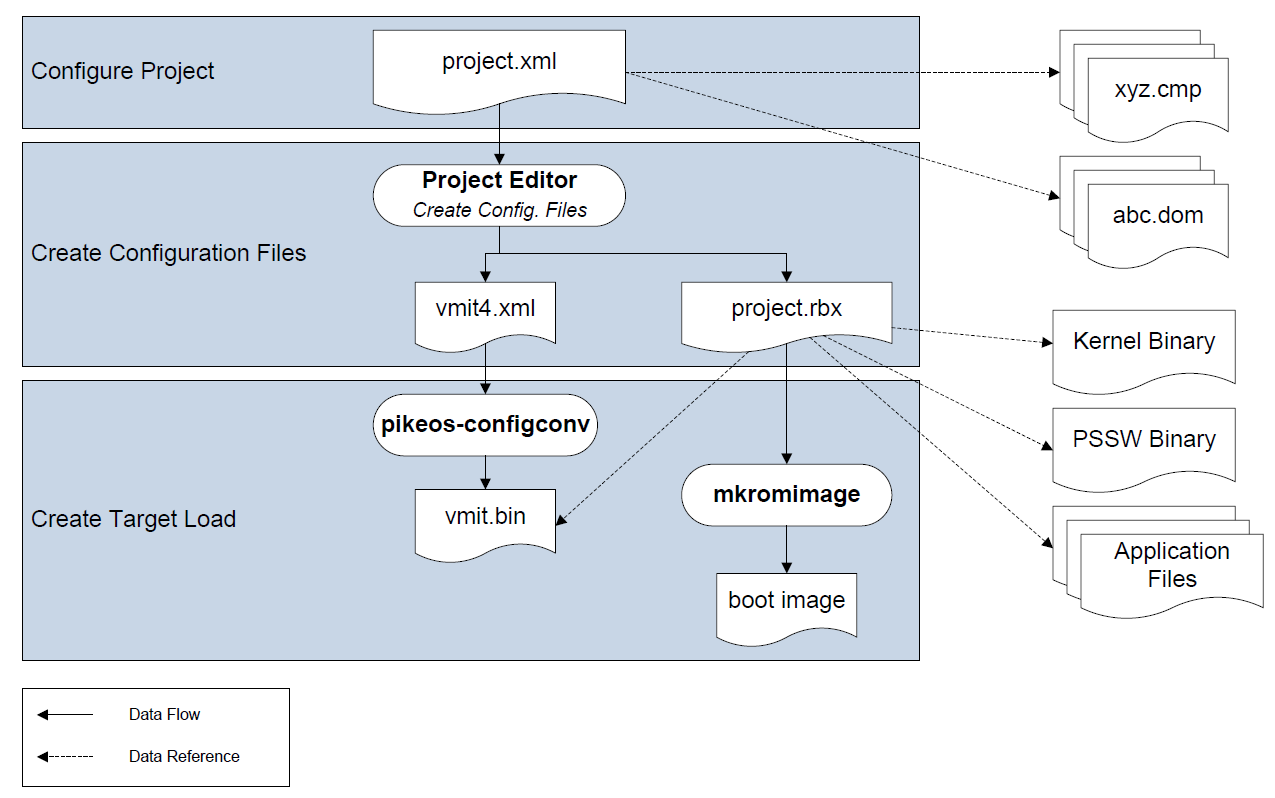
\includegraphics[width=1.0\textwidth]{PikeosProjectConfiguration}
\caption{PikeOS Project Configuration Overview}
\label{fig:PikeosProjectConfiguration}
\end{figure}

All the PikeOS relevant information are stored inside the \verb|project.xml| file. However, for lower level tools, the meta information inside this if file are not fully required; for that reason, the PikeOS Project Configurator converts the \verb|project.xml| file into the lower level configuration files used by the PikeOS system:
\begin{itemize}
\item \emph{ROM Boot Extended Configuration (RBX)} contains a description of the kernel, the memory region setup, the ROM file system and the file system;
\item \emph{Virtual Machine Initialization Table (VMIT)} contains all of the configuration settings of the PikeOS system and is used by the kernel to set up time and resource partitions as well as communication channels.
\end{itemize}
Both RBX and VMIT files are stored in XML format, but are converted to binary format before being loaded into the system.


%********************************** % Section  **************************************
\section{Simulink and Embedded Coder}
Simulink\textregistered \cite{Simulink}, developed by \emph{The MathWorks Inc.}, is a graphical programming environment for modeling, simulating and analyzing multidomain dynamic systems such as signal processing, control and communication applications. It supports system-level design, simulation, automatic code generation, and continuous test and verification of embedded systems. Thanks to its features, it is the \emph{de-facto} standard in model-based design.

\paragraph{} In order to generate C/C++ code from Simulink models, we can use \emph{Simulink Coder}\textregistered, formerly \emph{Real-Time Workshop}\textregistered. It supports code generation from both Simulink diagrams and Stateflow charts. Moreover; with Embedded Coder\textregistered, we can generate C/C++ code optimized to be used on embedded processors, on-target rapid prototyping boards, and microprocessors. It also provides traceability reports, code interface documentation, and automated software verification to assistance support standards such as DO-178 and ISO 26262 during development. It also supports external mode to connect the Simulink block diagram to the relative application that runs the model on the target hardware. The block diagram becomes a user interface to the real-time application, and by changing parameters in the Simulink blocks, the parameters in the real-time application also changes.

\subsection{Synchronous-Reactive Model of Computation}
Simulink implements a Synchronous-Reactive (SR) model of computation (MoC), and is used for the representation of systems in which components evolve synchronously, a fundamental concept for the modeling of concurrent systems \cite{Ptolemy2}. 
\par Synchronous-Reactive models are networks of Mealy-type blocks, eventually clustered into subsystems and can be continuous, discrete or triggered \cite{tres}. Continuous blocks process continuous-time signals and produce as output other continuous-signal functions according to the block description, typically a set of differential equations. Discrete-time blocks are activated at periodic-time instants and process input signals producing outputs signals and state updates. Finally, triggered blocks are only executed on the occurrence of a given event (a signal transition or a function call). 
\par Since we are interested in automatic code generation let us focus on discrete-time blocks which are (eventually) activated at each tick-time $t$. Let us denote a generic block $i$ as $B_i$, the input vector at tick-time $t$ as $\vec{u_i}(t)$ and similarly the output vector as $\vec{y_i}(t)$. Each block maintains a state vector $\vec{s_i}(t)$, and the behavior of $B_i$ is represented by its \emph{output update} function
\begin{equation}
\vec{y_i}(t)=f(\vec{u_i}(t),\vec{s_i}(t))
\end{equation}
and a \emph{state update} function
\begin{equation}
\vec{s_i}(t+1) = g(\vec{u_i}(t), \vec{s_i}(t))
\end{equation}
Often, the two update functions are considered as one:
\begin{equation}
(\vec{y_i}(t), \vec{s_i}(t+1)) = h(\vec{u_i}(t),\vec{s_i}(t))
\end{equation}

\paragraph{} A fundamental part of the model executable semantics are the rules dictating the evaluation order of the blocks. A block has a \emph{direct feedthrough} relationship between ports when the output port is controlled directly by the value of any input port signal. Any block with direct feedthrough relationship cannot execute until the block(s) driving its input has (have) executed. The set of topological dependencies implied by the direct feedthrough relationships defines a partial order of execution of the blocks. When the simulation starts, Simulink computes a total order of block execution compatible with the partial one.

\subsection{Real-Time Workshop Code Generation Process}
\label{sec:RTWGenerationProcess}
The Real-Time Workshop (RTW) simplifies the process of building application programs. One of its features is automatic program building, which provides a standard means to create programs for real-time applications in a variety of host environments. The functioning of RTW is fully customizable. The overall model build process is depicted in figure \ref{fig:RTWBuildProcess}.

\begin{figure}[htbp] 
\centering    
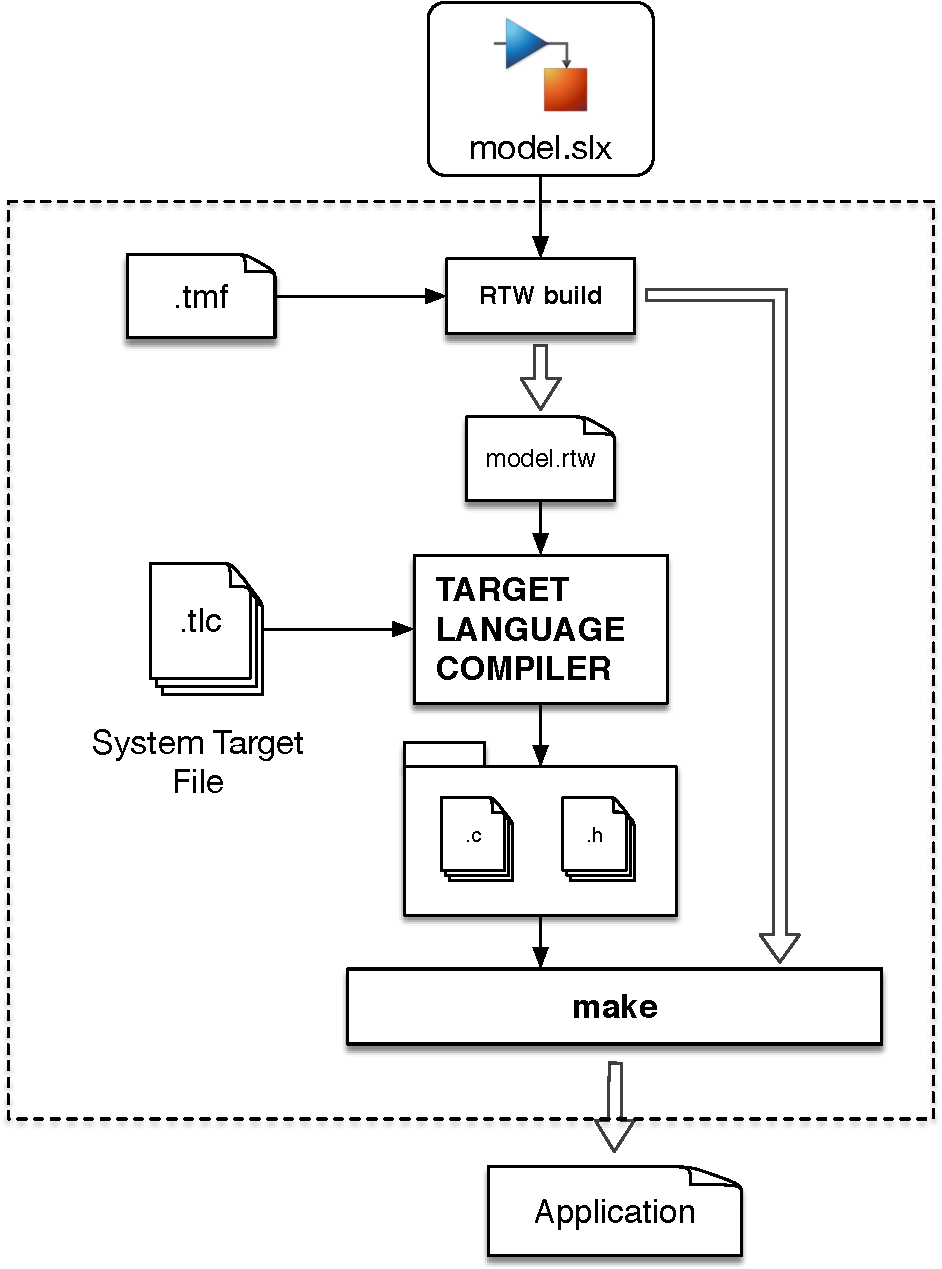
\includegraphics[width=0.45\textwidth]{RTWBuildProcess}
\caption{Real-Time Workshop Model Building Process}
\label{fig:RTWBuildProcess}
\end{figure}
The initial stage of the code generation process is to analyze the source model; the resulting description file, \verb|model.rtw| contains a \emph{compiled} representation of the model including a hierarchical structure of records describing systems, blocks, and their connections. This intermediate model description feeds the \emph{Target Language Compiler\textregistered} (TLC) that interprets it and guide the C/C++ code generation. It is also possible to write a \emph{Template Make File} (TMF) that define how to generate a Makefile for the actual compilation of the generated source files.

\paragraph{} The RTW file is a language-independent format, basically stored as an ASCII file. For example, consider the model depicted in figure \ref{fig:RTWModelExample}. An excerpt of the generated \verb|model.rtw| is in figure \ref{fig:RTWFileExample}.

\begin{figure}[htbp] 
\centering    
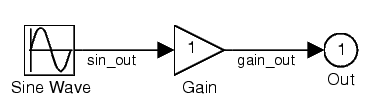
\includegraphics[width=0.4\textwidth]{RTWModelExample}
\caption{Model Example}
\label{fig:RTWModelExample}
\end{figure}

\begin{figure}[htbp] 
\centering    
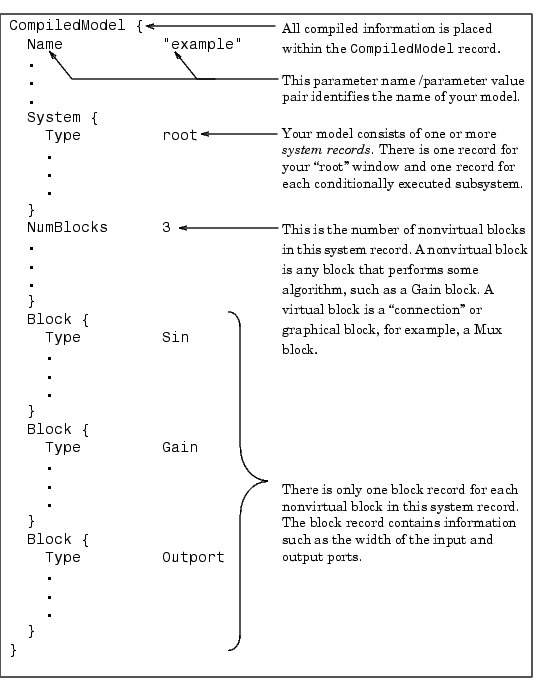
\includegraphics[width=1.0\textwidth]{RTWFileExample}
\caption{RTW File excerpt}
\label{fig:RTWFileExample}
\end{figure}

\subsubsection{Code Architecture}
\label{sec:CodeArchitecture}
When a model or a block is generated, the RTW follows a general structure for the generated code. Blocks have inputs, outputs, parameters, states, and other general properties. All Block inputs and outputs are written into a block I/O structure (\verb|rtXX|) and instantiated as global variables. Figure \ref{fig:TLCCodeStructure} shows the general block data mappings.
\begin{figure}[htbp] 
\centering    
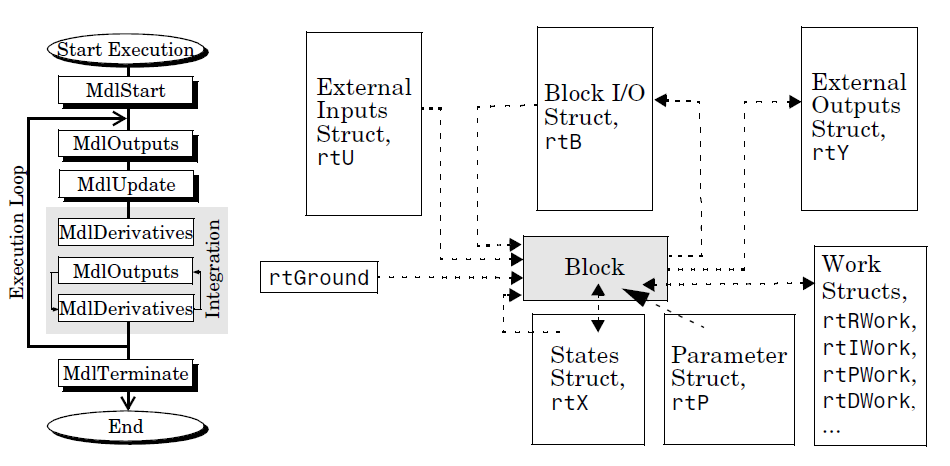
\includegraphics[width=1.0\textwidth]{TLCCodeStructure}
\caption{TLC Block code structure}
\label{fig:TLCCodeStructure}
\end{figure}
This structure applies also to the generated model. Out of the generation process, three \emph{Entry Point Functions} are available:%Embedded Coder pag 702
\begin{itemize} 
\item \emph{model\_initialize}. Model initialization entry point.
\item \emph{model\_step}. Step routine entry point.
\item \emph{model\_terminate}. Termination entry point.
\end{itemize}
The structures and the function are stored in the source code. Embedded Coder creates a build folder in the working folder to store the following generated source code:
\begin{itemize} % pag 51 RTW UG OR pag 592 Embedded Coder UG
\item \emph{model.c}. Contains entry point functions implementing the model algorithm.
\item \emph{model\_private.h}. Contains local macros and local data that are required by the model and subsystems. This file is included in the model.c file as a \verb|#include| statement.
\item \emph{model.h}. Declares model data structures,a public interface to the model
entry points and data structures. This file is included in the \verb|model.c| file.
\item \emph{model\_types.h}. Provides forward declarations for the data structure and the parameters data structure.
\item \emph{rtwtypes.h}. Defines data types, structures, and macros required by Embedded Coder generated code.
\item \emph{Optional files}. Sometimes additional source or header files are required by the generated code. These files are placed in the build folder.
\end{itemize}

\subsection{Concurrent Workflow}
Simulink provides a way to address the challenge of designing systems for concurrent execution through its \emph{Concurrent Workflow}. It uses the process of partitioning, mapping, and profiling to define the structure of the parallel application.
Partitioning enables to designate regions of the model as tasks. Mapping enables to assign partitions (tasks) to processing elements such as FPGAs or CPUs. Then Profiling simulates the deployment of the application under typical computational loads.
\begin{figure}[htbp] 
\centering    
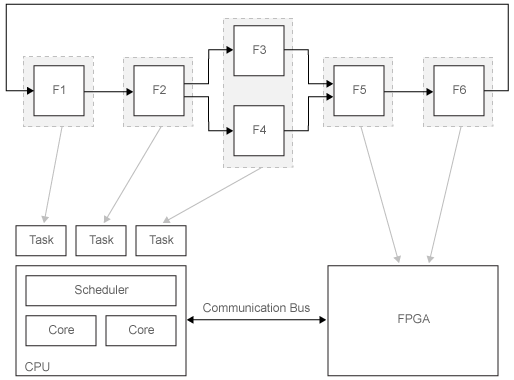
\includegraphics[width=0.8\textwidth]{SimulinkConcurrentWorkflow.png}
\caption{Simulink Multi-Core Partitioning}
\label{fig:SimulinkTaskPartitioning}
\end{figure}
%https://www.mathworks.com/help/simulink/ug/solving-embedded-performance-problems-using-multicore-processors-and-fpgas.html
%https://www.mathworks.com/help/simulink/ug/implicit-and-explicit-partitioning-of-models.html
\par Partitioning is the first step for defining the application's structure. There are two ways to partition the model for running on individual processing nodes.
The automated way of creating tasks and mapping them to processing nodes is called \emph{implicit partitioning}. Simulink partitions the model based on the sample times of blocks. Each sample time in the model corresponds to a partition, and all blocks activated with the same rate or sample time belong to the same partition. Then these partitions are mapped to tasks and their priority is assigned according to their rate. Therefore, implicit partitioning assumes the hardware architecture consists of a single multi-core CPU and that the Operating System scheduler handles all the execution according to task priorities.
\par Another way to specify partitions is to use \emph{explicit partitioning}. In explicit partitioning, partitions are created in the root-level model by using \emph{referenced models} (fig. \ref{fig:SimulinkTaskProfiling}). For example, if the model is made by a data acquisition and a controller, a possible partitioned model puts these components in two difference referenced models at the model root-level. Each sample time in a referenced model or a system block is a partition. Then using the \emph{Model Configurator}, in the Concurrent Execution dialog box, each task can be mapped to one processing node (by setting its affinity mask).
%https://www.mathworks.com/help/simulink/ug/implement-task-parallelism-in-simulink.html
\begin{figure}
  \begin{subfigure}{0.65\textwidth}
    \centering
    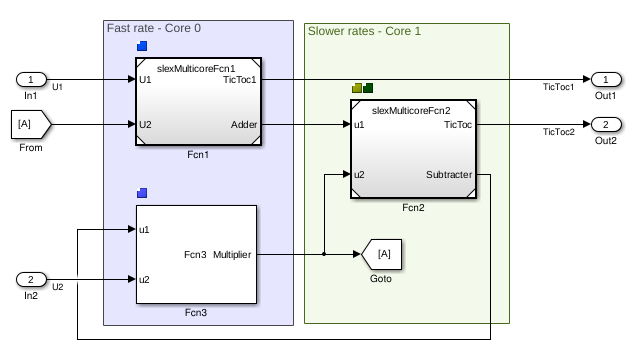
\includegraphics[width=1\textwidth]{slexMulticorePartitioning}
    \caption{Simulink Explicit Partitioning}
    \label{fig:slexPartitioning}
  \end{subfigure}%
  \begin{subfigure}{0.35\textwidth}
    \begin{subfigure}{\textwidth}
      \centering
      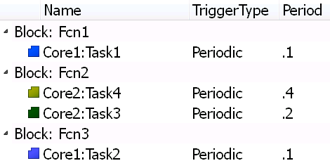
\includegraphics[width=1\textwidth]{slexMulticoreMapping}
      \caption{Simulink Mapping}
      \label{fig:slexMapping}
    \end{subfigure}
  \end{subfigure}
  \caption{Simulink Concurrent Workflow (by \emph{The Mathworks})}
  \label{fig:SimulinkTaskProfiling}
\end{figure}

\paragraph{} This tool is not yet mature, and complex to customize, for this reason, it does not suit well to mixed-critical applications. The aim of both implicit and explicit partitioning is the extraction of tasks by grouping blocks instead of finding a way to isolate functionality (robust partitioning). The automatic partitioning and mapping does not address the problem of safety and secure code execution. Instead, it focuses only on performance without any optimization. Even with explicit partitioning and mapping, the task priority assignment is rate-monotonic (tasks with shorter rate results in a lower priority) and does not take into account the Worst-Case Execution Time of tasks and the Resource usage. This information is critical for scheduling tasks while minimizing interferences and exploiting at best the task parallelism. Moreover, the whole process is strictly tied with the Simulink environment making difficult to integrate pieces of software developed by hand or automatically generated by other software.

\paragraph{} To overcome these limitations, one possible approach is to customize the code generation process. Simulink provides a configuration tool for this: the \emph{Target Language Compiler}. The following section briefly introduces it.

\subsection{Target Language Compiler}
The Target Language Compiler tool is part of the Real-Time Workshop. It enables the customization of the C/C++ code generated from any Simulink model or custom defined blocks. It has been designed for the purpose of converting the model description file, \verb|model.rtw|, into target-specific code.

\paragraph{} After reading the rtw file, the Target Language Compiler generates code based on \emph{target files}, which specify the source code implementation of each block and the overall code framework for the entire model. TLC works like a text processor, it has a mark-up syntax similar to HTML, along with the power of scripting languages, plus the data handling power of MATLAB (TLC can invoke MATLAB functions). All Simulink blocks are automatically converted to code (except MATLAB function blocks and S-function blocks that invoke M-files). 
\par In order to create a target-specific application, Real-Time Workshop also requires a template makefile that specifies the appropriate C compiler and its options for the build process. The template makefile is then transformed into a makefile (\verb|model.mk|) by performing \emph{token expansion} specific to a given model.

\paragraph{} Any rtw file contain a series of (usually hierarchically nested) \emph{records} in the form:
\begin{verbatim}
recordName {itemName itemValue}
\end{verbatim}
Item names are alphabetic. Item values can be strings or numeric values ( including scalars, vectors, and matrices). Curly braces set off the contents of each record, which may contain one or more items, delimited by space, tab, and/or return characters.
\par In an rtw file automatically generated from a Simulink model, the top-level (first) record’s name is \verb|CompiledModel|. Each block is represented by a subrecord within it, identified by the block name. The TLC, however, can parse any well-formed record file. For example, we can access:
\begin{lstlisting}
%% In tlc file you can:
/* Print a comment in the output file */
%assign genDate = CompiledModel.GeneratedOn
The Model Name is: <%CompiledModel.Name>
Generated on: %<genDate>
\end{lstlisting}
The first line is a comment; all text on a line following the characters \verb|%%| is treated as a comment (ignored, not interpreted or output). The text on the second line is printed in the file as it is.
\par The third line executes a TLC directive (because it starts with \verb|%|), the directive \verb|assign| creates a variable named \verb|genDate| and assigns a string value to it. The \verb|%assign| directive creates new and modifies existing variables. Its general
syntax is:
\begin{verbatim}
%assign [::]variable = expression
\end{verbatim}
The optional double colon prefix specifies that the variable being assigned to is a global variable. In its absence, a local variable in the current scope is created or modified.
\par The last two lines evaluate (expand) records. More precisely, the first line evaluates the field called \verb|Name| in the scope of \verb|CompiledModel|. The syntax \verb|%<expr>| causes the expression \verb|expr| (which can be a record, a variable, or a function) to be evaluated. This operation is sometimes referred to as an \emph{eval}.

\paragraph{} The previous statements do not print anything, because all outputs were directed to a null device (sometimes called the “bit bucket”). There is always one active output file, even if it is null. To specify, open, and close target files for code generation the following functions are available:
\begin{verbatim}
%openfile streamid [="filename"] [, mode]
%closefile streamid
%% Output operations ...
%selectfile streamid
\end{verbatim}
The \verb|%openfile| directive creates a file/buffer (in “w” mode), or opens an existing one (in “a” or “r” mode). The equal character is required for the specification of the output file name. Any number of streams can be open for writing, but only one can be active at one time. The directive can be used to switch between open files; they do not need to be closed until output operations to them actually end. When activated, \verb|STDOUT| directs output to the MATLAB command window.

\paragraph{} The \verb|%with| and \verb|%endwith| directive eases the burden of correctly coding TLC scripts and to clarify their context or scope. The syntax for their use is
\begin{verbatim}
%with RecordName
%% TLC stamements...
%endwith
\end{verbatim}
they can also be nested; for example it can be very useful while using \verb|foreach| loops to write
\begin{lstlisting}
%with CompiledModel
%with DataTypes
%foreach dt=NumDataTypes
Data Type Index = %<dt>
Data Type Name: %<DataType[dt].SLName>
%endforeach
%endwith
%endwith
\end{lstlisting}

\subsubsection{Counting Blocks and Subsystems}
As an example, the following TLC code counts the subsystems and blocks in the model.
\begin{lstlisting}
%% File: CountSubSysAndBlocks.tlc
%% Count blocks and subsystems of a model.rtw file
%%
%% NOTE: Change "<matlabroot>/" below to the
%% MATLAB main directory on your system
%addincludepath "<matlabroot>//rtw//c//tlc//lib" %%Enables TLC to find included files
%assign Accelerator = 0 %%Needed to avoid error in utillib
%include "utillib.tlc" %%Inserts one file in another, as in C (not used here)
%selectfile STDOUT
*** SYSTEMS AND BLOCKS IN RECORDFILE
%assign nbls = 0
%with CompiledModel
%foreach sysIdx = NumSystems
%with System[sysIdx]
%assign nbls = nbls + NumBlocks
*** %<NumBlocks> blocks in system %<sysIdx + 1>
%endwith
%endforeach
*** recordfile contains %<nbls> blocks in %<NumSystems> systems
%endwith
*** END LISTING
%% end CountSubSysAndBlocks.tlc
\end{lstlisting}
the script can be executed by writing in the command window
\begin{verbatim}
tlc -r model.rtw CountSubSysAndBlocks.tlc
\end{verbatim}
obtaining, for example
\begin{verbatim}
*** SYSTEMS AND BLOCKS IN RECORDFILE
*** 8 blocks in system 1
*** 10 blocks in system 2
*** 4 blocks in system 3
*** 7 blocks in system 4
*** 17 blocks in system 5
*** recordfile contains 46 blocks in 5 systems
*** END LISTING
\end{verbatim}


%********************************** % Section  **************************************
\section{Developed Framework}\label{sec:DevelopedFramework}
The aim of the thesis is to develop a framework to run different applications with different criticality levels in multi-core platforms ensuring adequate safety requirements. While the development of a robust optimal partitioning and scheduling algorithm is still an open problem, we focused on developing a code generation framework to implement, on PikeOS, a suitable scheme.
\par For this reason, we first developed a complete but relatively simple partitioning and a scheduling algorithm that extracts information from a Simulink model, lets the designer perform some configuration options and then provides an optimization engine for the allocation of the threads. The framework enables a full process flow for the automatic code generation of a mixed critical application. Figure \ref{fig:FrameworkOverview} shows the simplified design flow.
\begin{figure}[htbp] 
\centering    
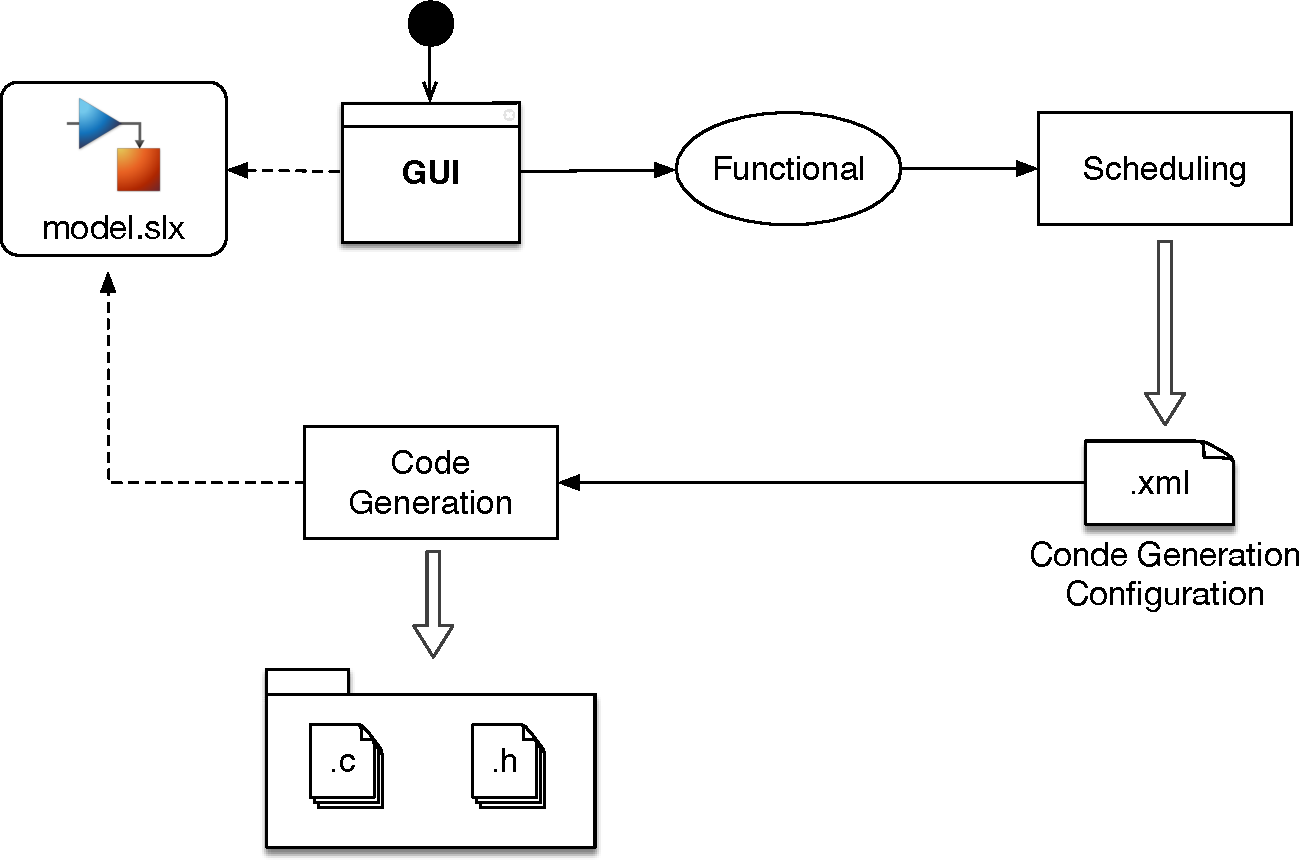
\includegraphics[width=0.7\textwidth]{FrameworkOverview}
\caption{Developed Framework overview}
\label{fig:FrameworkOverview}
\end{figure}
\par Once the models are developed and the simulation results are satisfactory, the system designer groups blocks in subsystems, which are considered as the unit of execution, such that there are no spare blocks among subsystems. Then a Matlab script uses the Simulink modeling API (programming interface) to parse the model structure and create a functional representation of the model to be utilized in the scheduling process (eventually exported as an XML). Finally, after the completion of the scheduling, the code generation process can start.

\subsection{Model Functional Representation}
A current challenge in the development of parallel applications is the achievement of a good scalability with the number of threads and processors. Often the scalability is heavily reduced by the precedence order of execution among threads (usually due to data dependencies). A possible approach to model the problem is through a \emph{Directed Acyclic Graph} (DAG). The DAG is a functional representation of the model, it consists of vertices (threads) and edges (communications/precedences) among nodes, with each edge directed from one vertex to another. The fact that it is an acyclic graph ensures that there is no \emph{algebraic loop} in the model. An algebraic loop occurs when a signal loop with only direct feedthrough blocks within it exist.
\par The designer can also add additional information to each node/thread such as
\begin{itemize}
\item Worst Case Execution Time (WCET) after performing some timing analysis on the subsystems\footnote{the subsystem will become a task, so this is the execution time related to a task.}. 
\item Criticality Level (A to E).
\item Resource Usage (a piece of resource like Shared Memory, UART, Ethernet, etc. can be defined and assigned to one or more threads).
\end{itemize}
This information is used by the engine to properly schedule threads on cores.
\par The functional model is created by a Matlab script that uses the Simulink modeling API (programming interface) to parse the model structure and create the DAG. It is based on the work of Matteo Morelli \cite{MorelliSee}. The Simulink model must comply with the restriction that:
\begin{enumerate}
\item The model consists of a collection of subsystems, with no spare blocks among them.
\item There are no continuous time blocks.
\item There are no multi-rate subsystems.
\end{enumerate}
These restrictions are a result of the fact that a C implementation should be generated from the model. 

\subsection{Partitioning and Scheduling Optimization}
The DAG represents a \emph{precedence graph} among threads, so it imposes a partial order of execution. To automatically generate an implementation (code generation) we must compute a total order among threads. This gap is an opportunity to improve safety and predictability (determinism) through partitioning and scheduling.

\paragraph{} In order to perform a real-time scheduling for the asks on multiprocessor platforms there exist two basic approaches: the \emph{partitioned approach}, in which each task is statically assigned to a single processor and migration is not allowed, and the \emph{global approach}, in which tasks can freely migrate and execute on any processor. Works from Gracioli\cite{Gracioli2013} and Melani\cite{Melani} shows a comparison of global scheduling and partitioned scheduling. Even though the global scheduling has several advantages, this thesis is focused on partitioned scheduling because the global scheduling would lead to preemptions and migrations, which produce more overheads and less determinism. In particular the latter might cause certification issues and this thesis wants reduce this possibility.

\par In this thesis we propose a general framework for a partitioned scheduling that can be mapped on PikeOS execution entities. For this purpose we identified several phases:
\begin{enumerate}
\item Mapping execution unit to tasks.
\item Task partitioning.
\item Task scheduling.
\item Priority assignment.
\item Partition scheduling.
\end{enumerate}
The scheduling process is implemented in Matlab as shown in figure \ref{fig:SchedulingProcess}.
\begin{figure}[htbp] 
\centering    
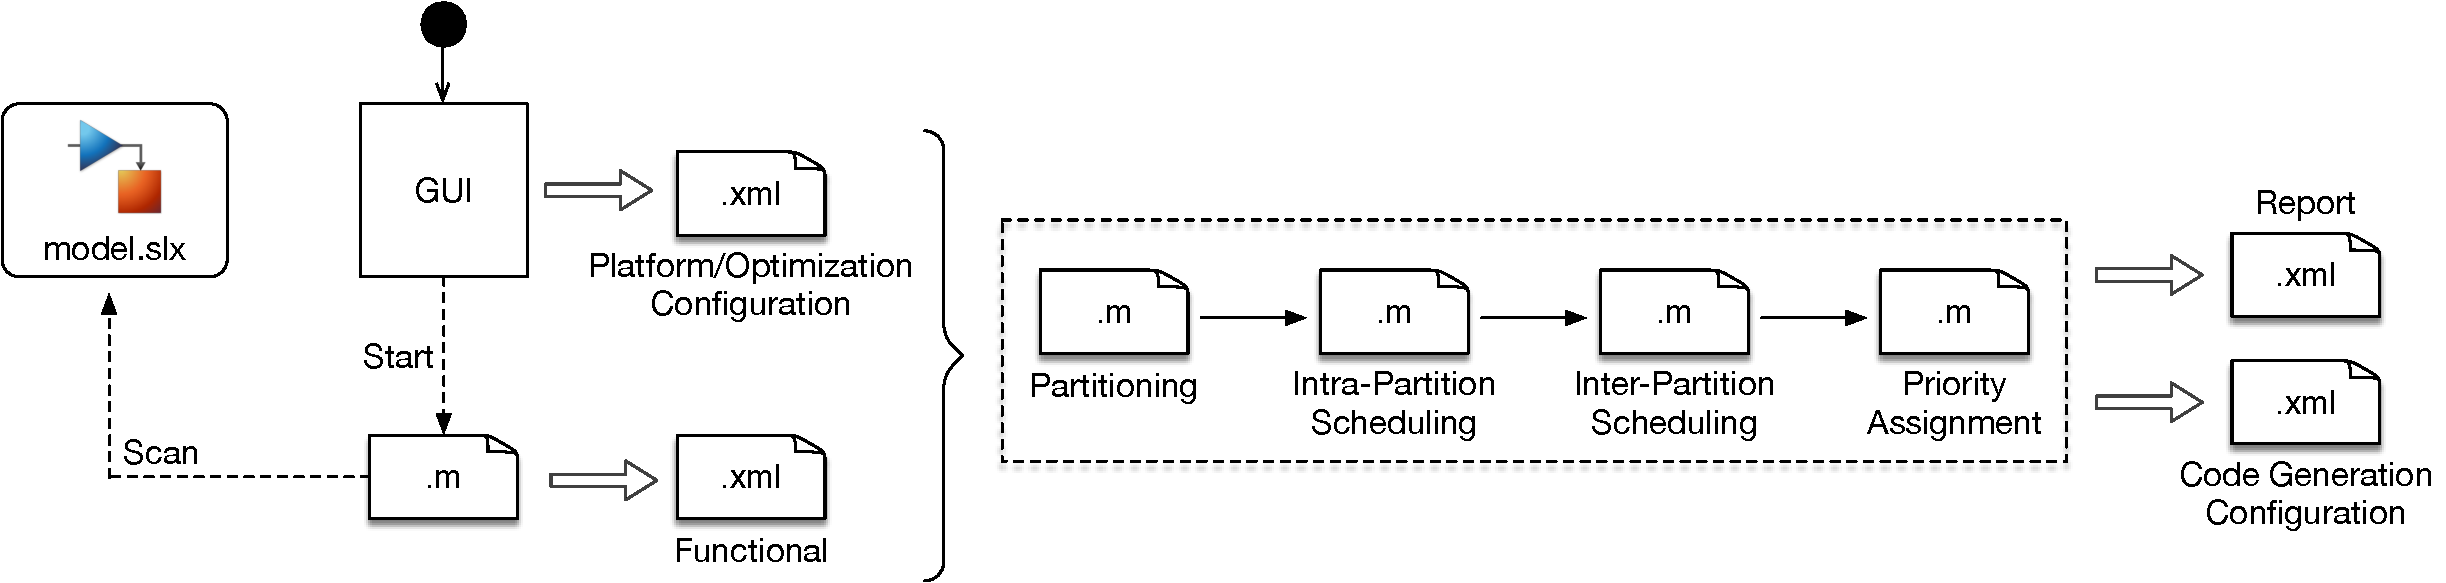
\includegraphics[width=1.0\textwidth]{SchedulingProcess}
\caption{Scheduling algorithm process}
\label{fig:SchedulingProcess}
\end{figure}

\subsection{Code Generation}
An optimal solution for the generation of code for mixed-criticality systems is not available from the literature. Since robust partitioning is the common way to address mixed-criticality, the code generation framework should take as input the description of such partitioned system. Recalling the fact that the code needs to be mapped into PikeOS execution entities, it is assumed that (with respect to PikeOS terminology) each Resource Partition is made by one Process with its threads and assigned to only one Time Partition. Obtaining the software architecture depicted in figure \ref{fig:SWArchitecture}.
\begin{figure}[htbp] 
\centering    
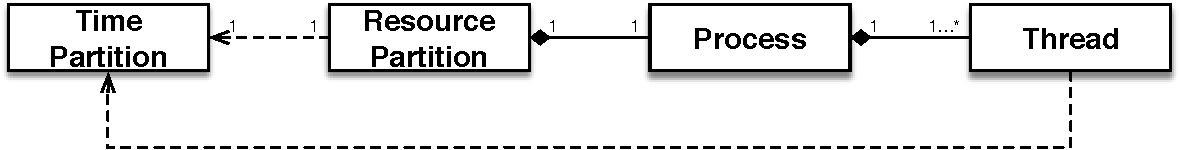
\includegraphics[width=0.9\textwidth]{SWArchitecture}
\caption{Software Architecture in the Developed Framework}
\label{fig:SWArchitecture}
\end{figure}
The reason why this architecture is proposed is that a different one would introduce further synchronization issues and less determinism. For example splitting a process in two separate processes, both assigned to the same resource partition would increase the possible interleaving among threads (basically all the possible states) and more synchronization calls for the communication. Moreover, since two processes (even if they are in the same Resource Partition) do not share the same virtual address space, more channels or additional shared memory regions must be defined. The same issues are caused if more than one Resource Partition is assigned to the same Time Partition.

\paragraph{} The underlying idea is to create a heterogeneous code generator partially independent from the platform. Since in this work the model representation is the Simulink Model, the code generation process is divided in two steps: \begin{enumerate}
\item Subsystems adaptation and generation: during this step Subsystem communications are eventually mapped to the right primitives (as defined in the code generation configuration file) and each Subsystem is generated with the Real Time Workshop/Embedded Coder as independent code.
\item System target code generation: here all the subsystems are glued together as threads, processes and partitions with target specific code.
\end{enumerate}
It can be noticed that the first step is OS agnostic if the communication primitives are an abstraction of the Operating System ones. The resulting code generation process is depicted in figure \ref{fig:CodeGenerationProcess}.
\begin{figure}[htbp] 
\centering    
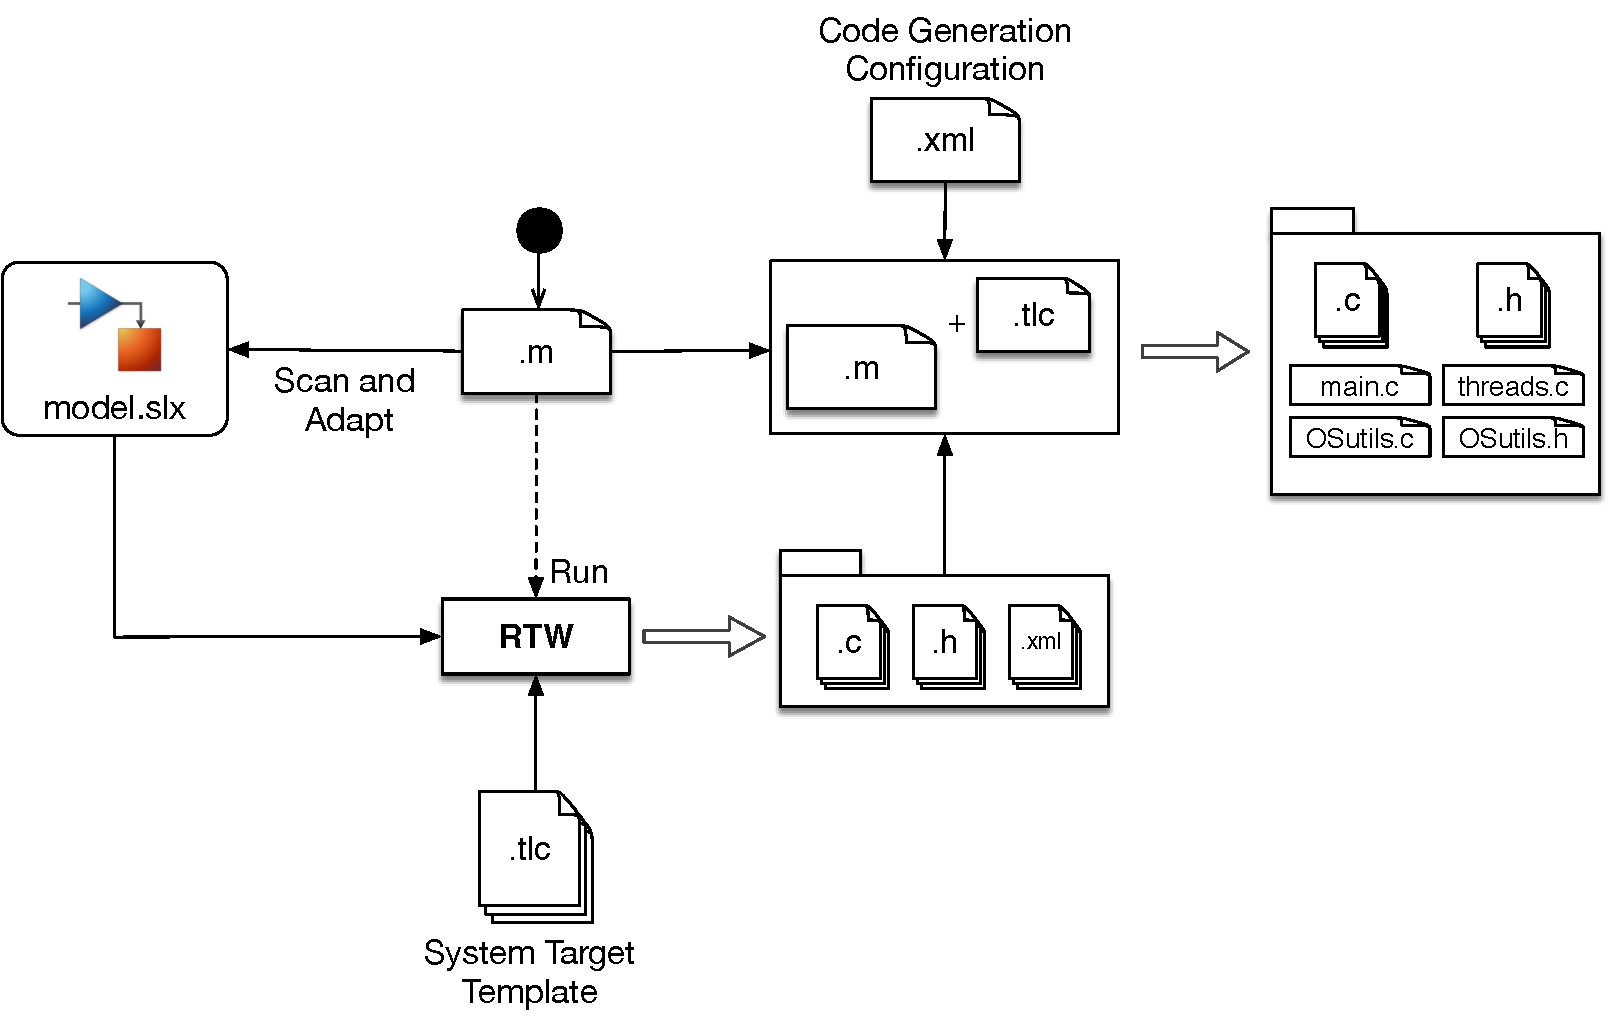
\includegraphics[width=0.8\textwidth]{CodeGenerationProcess}
\caption{Code generation process}
\label{fig:CodeGenerationProcess}
\end{figure}


% ~~~~~~~~~~~~~~~~~~~~~~~~~~~~~~~~~~~ % NTOES  ~~~~~~~~~~~~~~~~~~~~~~~~~~~~~~~~~~~
% The system runs different applications with different criticality levels, to reduce software complexity PikeOS is equipped with ARINC-653 compliant resource partitioning. The idea is to establish subsets of system resources, so-called “partitions”, serving as fault container: each program can only access its partition's own set of resources, so programs running in separate partitions cannot interfere with each other. Therefore, they do not need to trust each other and individual criticality levels can be assigned to each of them independently.
%PikeOS has been designed for use in safety-critical applications and has gone through a comprehensive validation according to safety standards like DO-178B, EN 50128, IEC 62304, IEC 61508,  ISO 26262, IEC 61513 for either the avionics, automotive, railway, medical, industrial automation or nuclear power plants. Since only the micro-kernel runs in privileged mode, all of its code contributes to the trusted code base of every application that might run on top of it. The effort of certifying a program is roughly proportional to the amount of code to be examined. This comprises the code of the program itself, but also that of the run-time environment (i.e. operating system, libraries etc.) which the program relies on. Therefore, the PikeOS micro-kernel consists of less than 10,000 lines of code making certification less expensive than that of conventional monolithic real-time operating systems. Even better: PikeOS allows the combination of applications of different levels of criticality where every application can be certified independently from others.

% https://www.sysgo.com/solutions/safety-security-certification/iso-26262/

%http://radio.feld.cvut.cz/matlab/toolbox/rtw/rtw_ug/tech_ov6.html
%!TEX root = ../thesis.tex

\chapter{Scheduling}

\ifpdf
    \graphicspath{{Chapters/Figs/Raster/}{Chapters/Figs/PDF/}{Chapters/Figs/}}
\else
    \graphicspath{{Chapters/Figs/Vector/}{Chapters/Figs/}}
\fi

%********************************** % Intro *****************************************
In this chapter a scheduling framework for mixed-critical applications with precedence constraint and communication costs is presented.

%********************************** % Section  **************************************
\section{Introduction}
\par It has been shown \cite{MCSNPhard} that the mixed-criticality schedulability problem (preemptive or non-preemptive) is strongly NP-hard even with only two criticality levels (High and Low). Nevertheless, different approaches had been proposed in the literature. The first research was presented in 2009 by Anderson et al.\cite{Anderson09} and extended in 2010 \cite{Mollison10}. The mechanism they presented is based on assigning to high-critical tasks higher Worst Case Execution Time and different scheduling policies (e.g. level A tasks are statistic assigned and cyclic released, level B with a Partitioned-EDF scheduler, level C and D with G-EDF). Kritikakou et al.\cite{Kritikakou14} provided a new scheduling for tasks distinguished in only two levels: HI-criticality and LO-criticality. Same as proposed by S.Baruah et al.\cite{Baruah2012EDFVD} in which they describe EDF-VD (for Earliest Deadline First with Virtual Deadlines)  for mixed-criticality tasks (see \cite{Zhang2014} for detailed analysis).

%\paragraph{} In the following sections is presented a model to schedule real-time, mixed-critical task-sets with precedence and periodicity through an off-line scheduling algorithm.
\paragraph{}To properly treat the problem an formal abstraction of the real-time scheduling with mixed-critical tasks with precedence and periodicity is presented.

%********************************** % Section  **************************************
\section{Problem Formulation}
As stated in the previous chapter, tasks (or threads) to be scheduled are represented as an acyclic directed graph. Every node in the graph represents one task and the edges between nodes, the communications. The node cost is the time required for the task to complete (WCET) and the edge cost is the communication cost. 

\paragraph{} More formally, the tasks are defined by $G=(\Gamma,E,C,T,K)$ where $\tau_i\in\Gamma$ represents a task and $\Gamma$ the task-set. The set $E=\{e_{ij}:\forall\tau_i\to\tau_j\}$ represent the precedence constraints between $\tau_i$ and $\tau_j$ (meaning that $\tau_i$ must be completed before $\tau_j$) with its communication cost expressed in time. The Worst-Case Execution Times are expressed in $C=\{c_i:\forall\tau_i\in\Gamma\}$. The periods (or rate) are $T=\{T_i:\forall\tau_i\in\Gamma\}$ and it is assumed that every $T_i$ is a integer multiple of some base-period $\beta_T$. The criticality levels are $K=\{\chi:\forall\tau_i\in\Gamma\}$. Moreover, each task has its priority $\rho_i$ which is assigned by the scheduling algorithm and a set of accessed resources $\mathbb{R}$ manually assigned by the system designer to each task.
\par The Direct Acyclic Graph made by all the partitions (which are the group of tasks) is denoted by $\mathbb{P}=(\Pi, H, L, R)$ and called \emph{P-DAG}, where $\pi_i\in\Pi$ is a partition. The inter-partition communications are represented in $H$, $\lambda_i\in L$ and $\delta_i\in R$ are respectively the duration and the periodicity of the partition $\pi_i$. So we can define a map $\Psi:\Gamma\to\mathbb{P}$ as the partitioning algorithm. The subgraph of $G$ made by all the tasks assigned to a given partition is called T-DAG.
\par The behavioral parameters for the task $\tau_i$ that the scheduling process must define are: the starting time $s_i$ (\emph{when} the task should execute), and the core $\mu_i$ on which it will execute (\emph{where} should execute), also called \emph{affinity mask}.

%********************************** % Section  **************************************
\section{Assumptions}
It is assumed that the COTS board is a connected network of processors with identical communication links (the Unified Memory Model shown in figure \ref{fig:unifiedmemorymodel}) and relatively small number of processors. This simplifies the mathematical formulation of the optimization problem and limits its computational complexity.
\par It is also assumed that the partitioning addresses the security and safety requirement. This mechanism relies on the Hypervisor, which is a trusted code (certified by the authorities) and it is the only one executing in the highest privileged mode. It ensures time and spatial isolation among partitions so the partitioning algorithm should map each task to one partition such that a fault in one partition does not affect another partition while considering the criticality as a decision variable. Moreover, interferences and  inter-partition communications should be minimized.

\paragraph{} Once partitions are determined, they need to be scheduled. The problem can be split in two parts: \emph{intra-partition} scheduling and \emph{inter-partition} scheduling. In the following sections is presented a detailed description of each phase.

%********************************** % Section  **************************************
\section{Partitioning}
Determine a way to measure safety is complex, hence, derive an optimization problem is not easy. In order to simplify the intra-partition scheduling and enforce determinism it is important that all the tasks inside a partition have the same period (or eventually integer multiple of the partition rate). To understand the rationale, assume that a task $\tau_i$ assigned to \TP{1} needs to be activated at time $t_1<t_{L_1}$ and $t_2>t_{L_2}$ as shown in figure \ref{fig:PartitionRationale}
\begin{figure}[htbp] 
\centering    
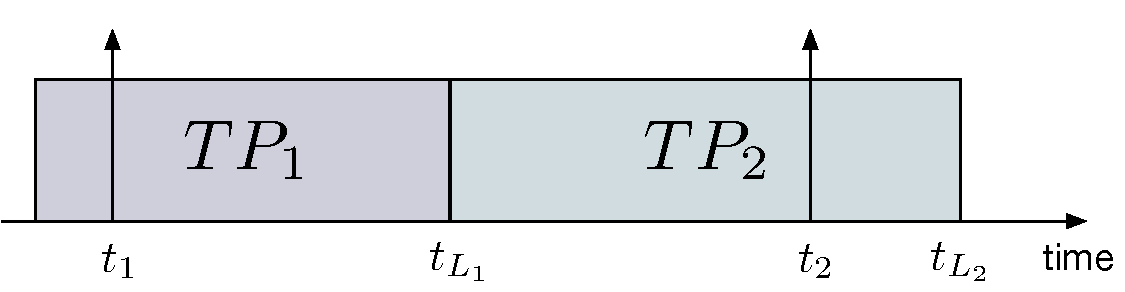
\includegraphics[width=0.7\textwidth]{PartitionRationale}
\caption{Non rate-base partitioning}
\label{fig:PartitionRationale}
\end{figure}

To allow this behavior, two approaches are possible:
\begin{enumerate}
\item Introduce preemption among time partition, losing determinism and the control of safety states.
\item Push the execution of $\tau_i$ o the new activation of \TP{1}. This approach leads to a lower level of determinism because $\tau_i$ now should interrupt any task assigned to \TP{2} that is executing at time $t_2$. Moreover, the worst-case execution time of \TP{2} will considerably change between different execution, leading to an over-estimating of it.
\end{enumerate}
The solution adopted in this work does not pretend to be a solution for the partitioning problem. Instead, it would be an example. The algorithm simply groups all the tasks with the same rates in partitions and then split them according to some criticality threshold, creating smaller sub-partitions. A more complex partitioning algorithm is under development.
\par As stated before, the result of the partitioning is another DAG, called P-DAG, each of them with its T-DAG. Now the inter-partition and intra-partition scheduling can be introduced. 

%********************************** % Section  **************************************
\section{Tasks Allocation and Scheduling}
\subsection{Intra-Partition}
In order to schedule partitions the execution time of the partition itself must be estimated. This optimization schedules a T-DAG on all the available $|M|$ processors. The solution space of this problem is spawned by all possible processor assignments combined with all possible task orderings that satisfy the partial order expressed by the T-DAG. The tasks are to be assigned in such a way as to minimize the total computation time required to execute that partition. This is also referred as reducing the makespan. The optimization problem that solves this problem presented below is based on the one proposed by S.Venugopalan and O.Sinnen \cite{ILP}.

\paragraph{} For each task $\tau_i\in\Gamma$, let $s_i$ the starting time, $\mu_i$ the core on which it will be executed and $\gamma_i$ the cost of all outgoing communications. Let $W$ the makespan and $|M|$ the number of available cores. Moreover, let $\delta^-(i)$ the set of tasks that need to be completed before task $\tau_i$. Some tasks cannot execute in parallel with another due the shared resource they are going to use, $\mathcal{I}$ is matrix that represent \emph{parallel incompatibilities}, the component $\mathcal{I}_{ij}$ is equal to one if $\tau_i$ and $\tau_j$ cannot execute in parallel, formally:
\[
\mathcal{I}_{i,j}=
\begin{cases}
1\quad \text{if } \tau_i \text{ and } \tau_j \text{ share at least one resource}\\
0\quad\text{otherwise}
\end{cases}
\]
Let the variable $x_{ik}$ is one if task $\tau_i$ is assigned to the processor $\mu_k$, zero otherwise. In order to control the scheduling behavior, define the following set of binary variables:
\[
\forall \tau_i,\tau_j\in\Gamma \quad \sigma_{ij}=
\begin{cases}
1\quad s_i+c_i\leq s_j \\
0\quad\text{otherwise}
\end{cases}
\]
\[
\forall \tau_i,\tau_j\in\Gamma \quad \epsilon_{ij}=
\begin{cases}
1\quad\mu_i<\mu_j \\
0\quad\text{otherwise}
\end{cases}
\]
The resulting MILP problem is
\begin{align}
\min    										& \quad & W \label{eq:milp1}\\
\forall\tau_i\in\Gamma							&  &  s_i+c_i\leq W \label{eq:milp2}\\
\forall\tau_i\neq\tau_j\in\Gamma				&  &  s_j-s_i-c_i-\gamma_i-(\sigma_{ij}-1)W_{\max}\geq 0 \label{eq:milp3}\\
\forall\tau_i\neq\tau_j\in\Gamma				&  &  \mu_j-\mu_i-1-(\epsilon_{ij}-1)M\geq 0 \label{eq:milp4}\\
\forall\tau_i\neq\tau_j\in\Gamma				&  &  \sigma_{ij}+\sigma_{ji}+\epsilon_{ij}+\epsilon_{ji}\geq 1 \label{eq:milp5}\\
\forall(i,j):\mathcal{I}_{ij}=1 				&  &  s_i+c_i+\gamma_i-s_j\leq W_{\max}(1-\sigma_{ij}) \label{eq:milp6}\\
\forall(i,j):\mathcal{I}_{ij}=1					&  &  s_j+c_j+\gamma_j-s_i\leq W_{\max}\sigma_{ij} \label{eq:milp7}\\
\forall\tau_i\neq\tau_j\in\Gamma				&  &  \sigma_{ij}+\sigma_{ji}\leq 1 \label{eq:milp8}\\
\forall\tau_i\neq\tau_j\in\Gamma				&  &  \epsilon_{ij}+\epsilon_{ji}\leq 1 \label{eq:milp9}\\
\forall\tau_j\in\Gamma:\tau_i\in\delta^-(j)		&  &  \sigma_{ij}=1 \label{eq:milp10}\\
\forall\tau_i\in\Gamma 							&  & \sum_{k\in |M|} kx_{ik}=\mu_i \label{eq:milp11}\\
\forall\tau_i\in\Gamma 							&  & \sum_{k\in |M|} x_{ik}=1 \label{eq:milp12}\\
												&  & 0\leq W \leq W_{\max} \label{eq:milp13}\\
\forall\tau_i\in\Gamma 							&  & s_i\geq 0 \label{eq:milp14}\\
\forall\tau_i\in\Gamma 							& & \mu_i\in \{1,...,|M|\} \label{eq:milp15}\\
\forall\tau_i\in\Gamma,k\in |M|					& & x_{ij}\in\{0,1\} \label{eq:milp16}\\
\forall\tau_i,\tau_j\in\Gamma					& & \sigma_{ij},\epsilon_{ij} \in\{0,1\} \label{eq:milp17}
\end{align}
Where $W_{\max}$ is an upper bound for the makespan $W$. It can be computed as all the tasks were executed on a single core (so it is the sum of computational cost and communication costs) or with some heuristics. 
\par The formulation is a min-max problem: this is achieved by minimizing the makespan $W$ while introducing the constraint (\ref{eq:milp2}). Constraint (\ref{eq:milp3}) impose the partial order on the tasks in terms of the $\sigma$ variables. Constraint (\ref{eq:milp4}) impose the multi-core usage. Constraint (\ref{eq:milp5}) impose that at least one of the following is true: $\tau_i$ must finish before $\tau_j$ starts and/or $\mu_i<\mu_j$. Constraints (\ref{eq:milp6}) and (\ref{eq:milp7}) avoid that two tasks that share a common resource execute in parallel. By (\ref{eq:milp8}) and (\ref{eq:milp9}) a task cannot be before and after another task in both time and cores. Constraint (\ref{eq:milp10}) enforces the task precedences defined by the T-DAG. Constraints (\ref{eq:milp11}) link the assignment variable $x$ with the core variables $\mu$ and finally (\ref{eq:milp12}) ensures that any given task runs only on one core.
\par The complexity in terms of constraint and variables, depends on $|G|$, $|E|$, $|M|$ and $|\mathcal{I}|$. Assuming that the number of processor $|M|$ and the number of shared resources $|\mathcal{I}|$ are small, then the MILP complexity is dominated by (\ref{eq:milp10}) which generates $O(|G||E|)$ constraints. In the worst case scenario $|E|=|G|(|G|-1)/2$, however, for task-sets representing real applications, we usually have $O(|E|)=O(|G|)$, hence the overall complexity is $O(|G|^2)$.

\paragraph{} Once a T-DAG related to a partition is scheduled the makespan of the schedule is the Worst-Case Execution Time of the partition itself. Moreover, the variables $s_i$ and $\mu_i$ for each task $\tau_i\in\Gamma$ are known so the priorities can be computed.

\subsection{Inter-Partition}\label{interpartition}
The inter-partition schedule is analogue to the problem of schedule the P-DAG on a single core. Indeed, each Resource Partition is assigned to a Time Partition that is as big the total Worst-Case-Execution-Time of the Resource Partition contained (this amount of time can be estimated after the intra-partition schedule). In PikeOS, Time partitions are scheduled according to a statically-assigned schedule scheme like they were on a single core.
\par The problem of scheduling tasks on a single core have received substantial attention and many algorithms are available in the literature, for a complete review see \cite{buttazzoRT} and \cite{blazewiczScheduling}.

\paragraph{} When scheduling the P-DAG, the partial order expressed by it must be satisfied. Let introduce some concept (as in \cite{blazewiczScheduling}). For seek of notation simplicity, let consider a partition like a task, so that the same notation as before can be used. In addition to the previous notation, let introduce the \emph{arrival time} of a partition $\pi_i$ as $r_i$ which represent the moment in time in which a partition can start its execution, and the \emph{due date} $\widetilde{d}_i$ as the moment in time in which the task must be completed. These parameters, together with the periodicity, represent the real-time requirement for a given partition.

\subsubsection{Factorization}
Considering all nodes in the P-DAG, it is common to find different periodicity. In the general problem formulation is assumed that the periodicity of each task is an integer multiple of a base-period $\beta_T$, so when they are grouped into a partition, the partition itself inherit the rate of the tasks it contains and the so does the property. If $T_i=k_i\beta_T$ , the \emph{Hyper-Period} or \emph{Major Time Frame} can be defined as
\begin{equation}
\Delta = \gcd(k_1,k_2,...)\beta_T\quad i=\{1,...,|\Pi|\}
\end{equation}
Inside the hyper-period some partitions $\pi_i$ should execute more than once, in general exactly $k_i$ times. In order to generalize this behavior, a \emph{factorized P-DAG} can be defined. Let denote it as $\widetilde{\mathbb{P}}=(\widetilde{\Pi},\widetilde{H},\widetilde{L},\widetilde{R})$, it is a \emph{finite repetitive precedence} of partition $\pi_i$ by exactly $k_i$ times, in a direct precedence relation. The factorization process is depicted in figure \ref{fig:Factorization}.

\begin{figure}[htbp] 
\centering    
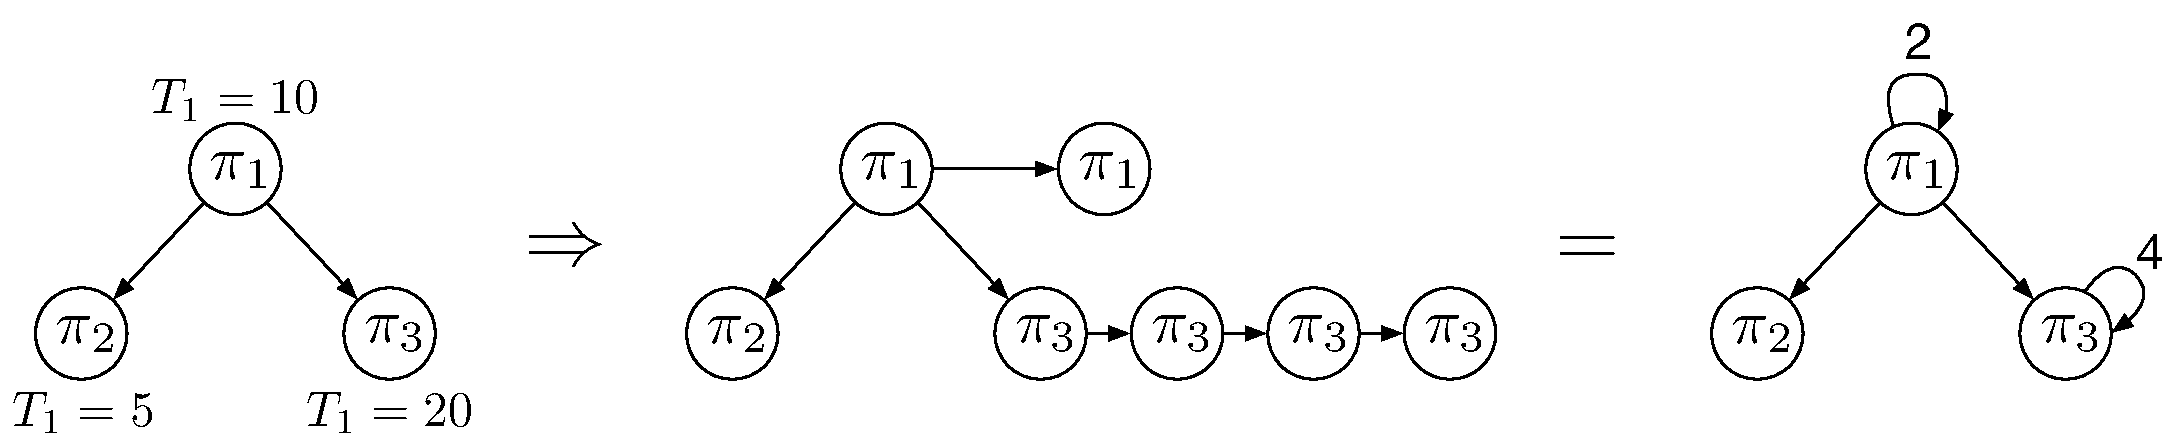
\includegraphics[width=1.0\textwidth]{Factorization}
\caption{Factorization example}
\label{fig:Factorization}
\end{figure}

\subsubsection{Partitions precedence constraints}
\par Given a schedule, it is called \emph{normal} if, for any two partition $\pi_i,\pi_j\in\Gamma$, $s_i<s_j$ implies that $\widetilde{d}_i\leq\widetilde{d}_j$ or $r_j>s_i$. Release times and deadlines are called \emph{consistent with the precedence relation} if $\pi_i\to\pi_j$ implies that $r_i+\delta t\leq r_j$ and $\widetilde{d}_i\leq\widetilde{d}_j-\delta t$, where $\delta t$ represent a small amount of time (basically the scheduling decision tick-time). The following lemma proves that the precedence constraints are not of essential relevance if there is only one processor.
\begin{lemma}\label{eq:precedenceLemma}
If the release times and deadlines are consistent with the precedence relation, then any normal one-processor schedule that satisfies the release times and deadlines must also obey the precedence relation. 
\end{lemma}
\begin{proof}
Consider a normal schedule, and suppose that $\pi_i\to\pi_j$ but $s_i>s_j$. By the consistency assumption we have $r_i<r_j$ and $\widetilde{d}_i<\widetilde{d}_j$. However, these, together with $r_j\leq s_j$, cause a violation of the assumption that the schedule is normal, a contradiction from which the result follows.
\end{proof}
This lemma ensures that release times and deadlines can be made consistent with the precedence relation if they are redefined by:
\begin{align}\label{eq:precedence}
r^{'}_{j} = & \max\big(\{r_j\}\cup\{r^{'}_i+\delta t:\pi_i\to\pi_j\} \big) \\
\widetilde{d}^{'}_j = & \min\big(\{\widetilde{d}_j\}\cup\{\widetilde{d}^{'}_i-\delta t:\pi_j\to\pi_i\} \big)
\end{align}
%\begin{align}
%r^{'}_{\alpha_j} = & \max\big(\{r_{\alpha_j}\}\cup\{r^{'}_{\alpha_i}+\delta t:\pi_{\alpha_i}\to\pi_{\alpha_j}\} \big) \\
%\widetilde{d}^{'}_{\alpha_j} = & \min\big(\{\widetilde{d}_{\alpha_j}\}\cup\{\widetilde{d}^{'}_{\alpha_i}-\delta t:\pi_{\alpha_j}\to\pi_{\alpha_i}\} \big)
%\end{align}
These changes do not alter the feasibility of any schedule. Furthermore, from lemma \ref{eq:precedenceLemma} follows that a precedence relation is essentially irrelevant when scheduling on one processor. 

\subsubsection{Bratley algorithm}
Scheduling partitions with precedence constraint (or adapted arrival times and due dates) is NP-hard in the strong sense, even for integer release times and deadlines \cite{LRKB77}. Only if all tasks have unit processing times, an optimization algorithm of polynomial time complexity is available. However, Bratley et al. \cite{bratleyScheduling} proposed a branch-and-bound algorithm which solves this class of problems. Their algorithm is shortly described below.
%Scheduling Computer and Manufacturing: Bratley et al. [BFR71] , page 74
\begin{figure}[htbp] 
\centering    
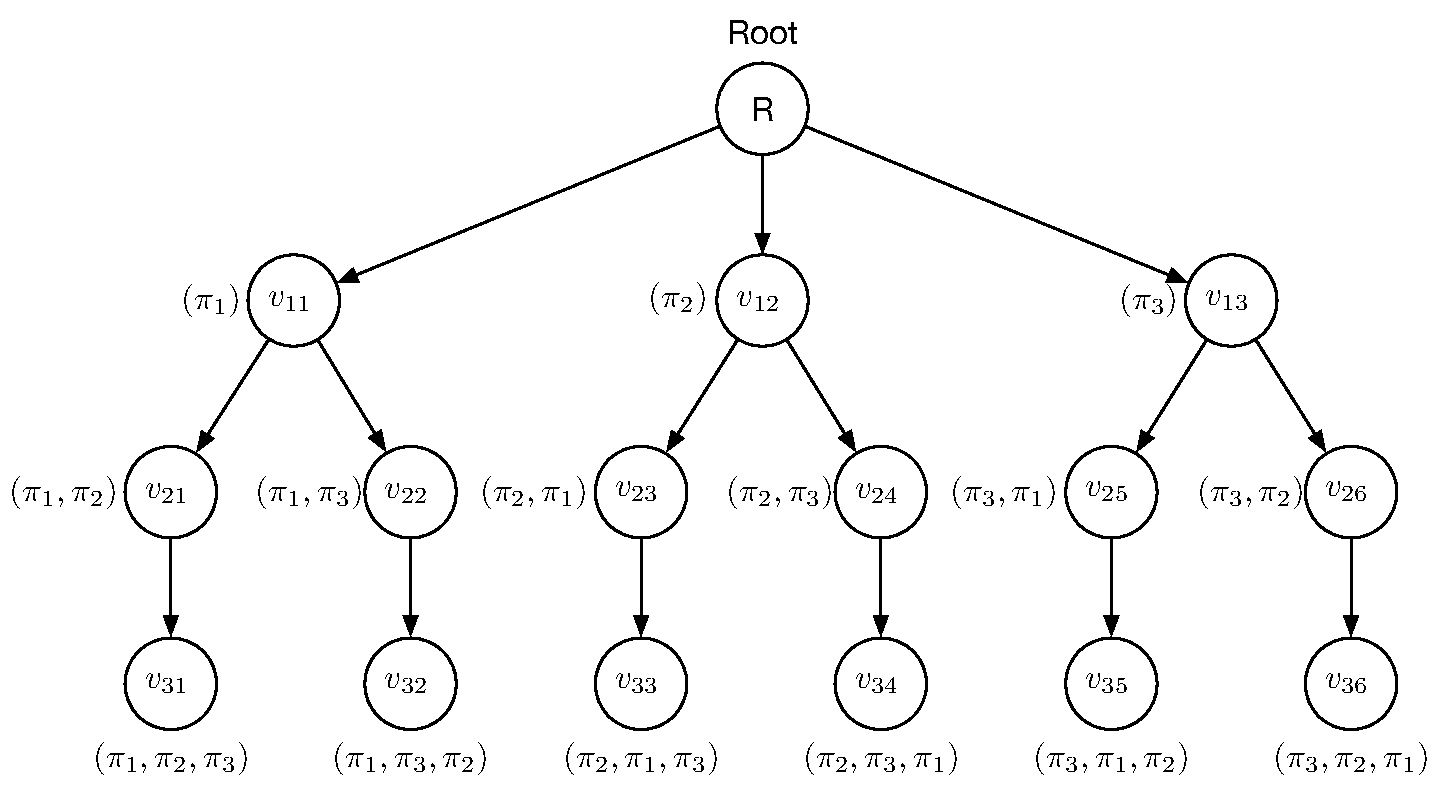
\includegraphics[width=1.0\textwidth]{Bratley}
\caption{Search tree example for Bratley et al. algorithm}
\label{fig:bratley}
\end{figure}
\paragraph{} All possible partition schedules are implicitly enumerated by a search tree as shown in Figure \ref{fig:bratley} (for three partitions). Each node $v_{ij}$ of the tree represents the assignment of $i-1$ partitions and a new unscheduled one to be in the $i$-th position of the schedule scheme, with $i = \{1,...,N\}$, $N=|\widetilde{\mathbb{P}}|$. On each level $i$, there are $N-i+1$ new nodes generated from each node of the preceding level. Hence, all the $N!$ possible schedule will be enumerated. To each node is associated the completion time of the corresponding partial schedule.
\par The order in which the nodes of the tree are examined is based on a \emph{backtracking
search strategy}. Moreover, the algorithm uses two criteria to bound the solution space.
\begin{enumerate}
\item Exceeding deadlines. Consider a node $v_{ij}$ of the tree where one of the $i$ partitions exceed its due date, it will certainly exceed its deadline if other partitions are scheduled after it. Therefore, the node with all the sub-tree may be excluded from further consideration.
\item Problem decomposition. Consider a node $v_{ij}$ where an unscheduled partition is assigned to $i$-th position of the schedule scheme. If the completion time of this partial schedule is less than or equal to the smallest release time among the yet unscheduled partitions, then the problem decomposes at level $i$, and there is need to backtrack beyond level $i$. This follows from the fact that the best schedule for the remaining $N-i$ partitions may not be started before the smallest of their release times.
\end{enumerate}
After enumerating all the possible $N!$ the best schedule according to an objective function can be selected. A common objective function is the makespan minimization.

%If the objective function is the makespan minimization, a sufficient but not necessary condition for optimality can be derived. Let define a \emph{block} as a group of partitions such that the first partition starts at its release time and all the following partitions to the end of the schedule are processed without idle times. Thus the length of a block is the sum of processing times of the partition within that block. If a block has the property that the release times of all the partitions within the block are greater than or equal to the release time of the first partition in the block (in that case we will say that \emph{"the block satisfies the release time property"}), then the schedule found for this block is clearly optimal. A block satisfying the release time property may be found by scanning the given schedule, starting from the last partition and attempting to find a group of tasks of the described property. Then, from the definition follow the lemma
%\begin{lemma}
%If a schedule for for a single-core, with starting time and due date, satisfies the release time property then it is one optimal solution for the makespan minimization.
%\end{lemma}

%********************************** % Section  **************************************
\section{Priority assignment}\label{sec:priorityassignment}
Priority assignment is required to allow the operating system scheduler to execute tasks according to the optimal schedule. 
\par Let assume that each thread has its affinity mask, meaning that it can execute only on the core specified by it and that the scheduler is priority-based FIFO queue. To enforce the non-preemptive behavior for the tasks inside a partition, threads on the same core must have \emph{strictly monotonically decreasing} priorities. Here to derive a correct assignment algorithm, an assumption on the implementation is required. Priorities alone cannot ensure mutual exclusion on communications memory locations. These shared memory regions are accessed only by communicating thread and them can be placed:
\begin{itemize}
\item On the same core: so priorities can ensure that the inputs are fulfilled, indeed the task with lower criticality will not execute before higher priority task.
\item On different core: so spinlocks can be used.
\end{itemize}
The use of spinlocks for inter-core synchronization is suggested because they avoid overhead from operating system process rescheduling or context switching. Moreover, spinlocks are efficient if tasks are likely to be blocked for only short periods, which is true to a certain degree that depends on the worst-case timing analysis. 

\paragraph{} A simple yet effective way to achieve this result is through a Linear Programming optimization problem:
\begin{equation}
\begin{cases}
\min \sum\rho_i \\ 
\rho_i - \rho_j \leq -1 \quad
\begin{matrix}
\text{for each consecutive task } \tau_i,\tau_j \text{ on the same core} \\
\text{for each communication edge } e_{ij} \text{ between cores}
\end{matrix} \\
\rho_{\min} \leq \rho_i \leq \rho_{\max}
\end{cases}
\end{equation}
where $\rho_i$ is the priority assigned to task $\tau_i\in\Gamma$. This class of problems can be solved in polynomial time \cite{polyLP}.

\paragraph{} Usually an operating system can only handle a finite set of priority values, for this reason the variable $\rho$ is bounded. However, if the schedule priority assignment does not use all the possible priority values, it is possible to create a gap below and above the partition to allow the execution of sporadic tasks. For example, this behavior can be easily implemented utilizing the background PikeOS partition \TP{0}. The result is depicted in figure \ref{fig:PriorityAssignment}.

\begin{figure}[htbp] 
\centering    
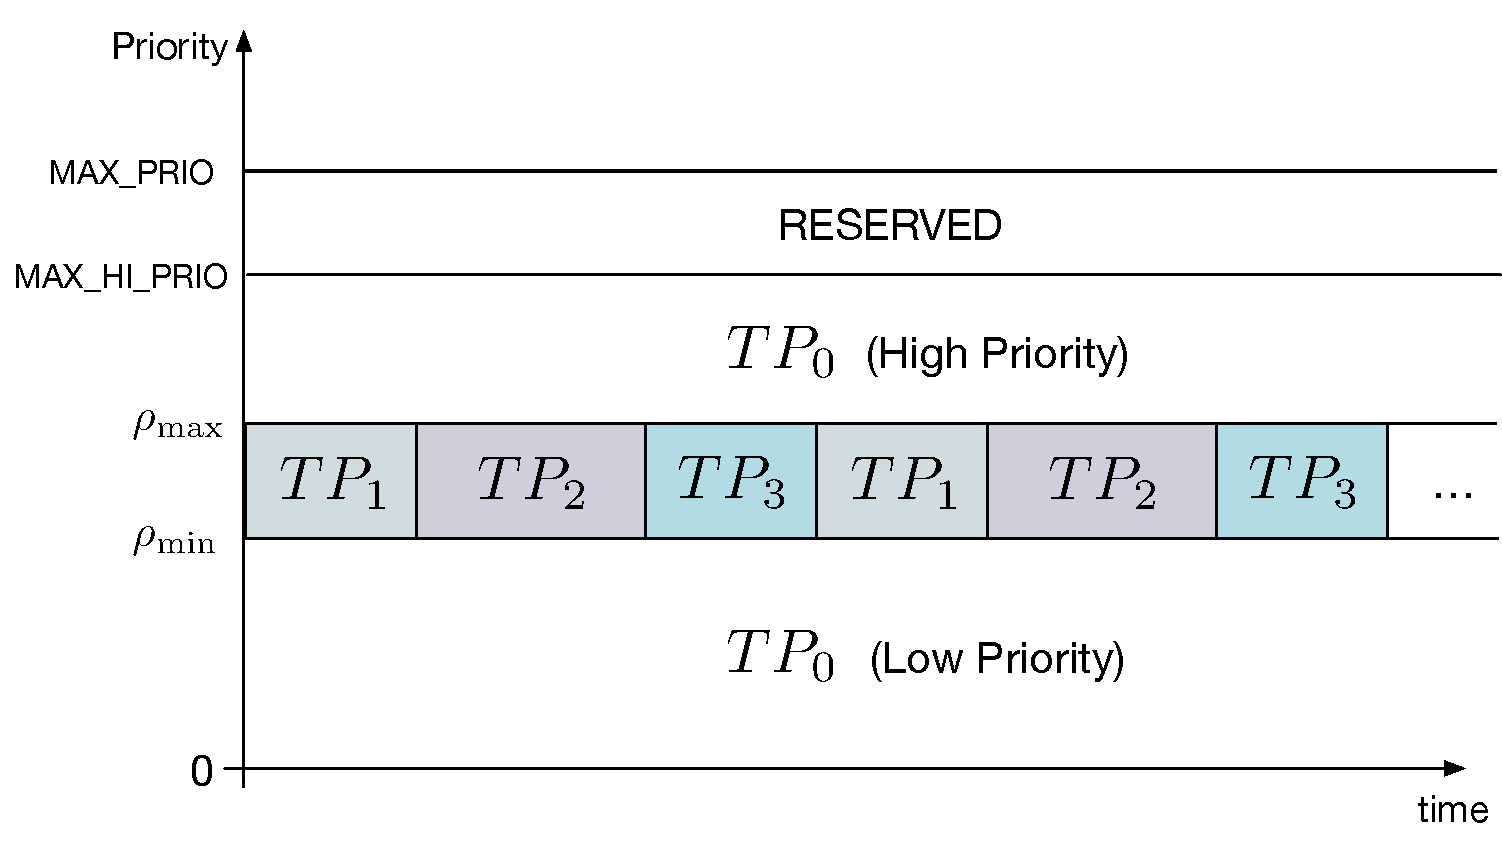
\includegraphics[width=1.0\textwidth]{PriorityAssignment}
\caption{Priority Assignment }
\label{fig:PriorityAssignment}
\end{figure}

%!TEX root = ../thesis.tex

\chapter{Code Generation}

\ifpdf
    \graphicspath{{Chapters/Figs/Raster/}{Chapters/Figs/PDF/}{Chapters/Figs/}}
\else
    \graphicspath{{Chapters/Figs/Vector/}{Chapters/Figs/}}
\fi

%********************************** % Intro *****************************************
Software development for embedded systems is increasingly being done with the help of block diagram specifications, simulation tools, and automatic code generation. With the growing importance of multi-core processors in safety-critical systems, there is also an increasing need for certification-compliant and time-predictable implementation via code-generation. In this chapter the code generation framework for Simulink is presented.

%********************************** % Section  **************************************
\section{Code-Generation Configuration}\label{sec:modelAdapt}
Before starting the code generation process, some configuration is required. In particular, the code generator needs to know about the software architecture, i.e.:
\begin{itemize}
\item \emph{Partitions}. The number of Partitions and their properties such as the duration and the number of activations.
\item \emph{Threads}. The DAG enriched with the information coming from the scheduling (affinity mask, priority and partition).
\end{itemize}
The current implementation expects an XML file (which is automatically generated by the developed scheduling framework) containing the  information as shown in the following example of the configuration file:
% CODE FRAGMENT
\lstinputlisting{Chapters/SrcCode/CodeConf.xml}
This file is parsed by a Matlab script and represented as a hierarchical class structure in the workspace. The resulting object is used by the next steps. 

%********************************** % Section  **************************************
\section{Model Configuration for Code Generation}
Once the configuration is loaded, a Matlab script adapt the model to implement the software architecture described in the configuration file. In particular, it has to address the communication issue.
\par All the threads inside a process share the same virtual memory address space, so a global variable containing an output (or input) of a thread is accessible from every thread. When the threads are scheduled inside two different partitions, this variable is no longer accessible. For solving this problem, two approaches are possible:
\begin{enumerate}
\item \emph{Communication Primitives}. Use message oriented communication such as Sampling or Queuing Ports.
\item \emph{Shared Memory Regions}. Define shared memory regions between the two partitions.
\end{enumerate}
While shared memory is suitable for a large amount of data, usually a single inter-partition communication channel, which is the implementation of a Simulink Line, transfers a limited amount of bytes. This lead to the use of communication primitives. As explained in section \ref{sec:CommPorts}, Queuing ports implement buffered communication while Sampling ports always contain the freshest value and its validity flag with respect to the expected refresh rate. This last capability is very useful to understand if a fault occurred to one of the predecessors of the executing thread, and eventually implement some handler for a not up-to-date value. For this reason, Sampling Ports are used as Inter-Partition Communications.

\paragraph{} Therefore, every subsystem's Outports and Inports that are at the edge of two different partitions must be replaced by the relative operation on the Sampling port. For this reason, a \emph{Custom Block} for each operation has been developed.

\subsection{Custom Blockset for Sampling Ports}
Any Inport and the Outports (which are blocks) that implement an inter-partition communication need to be substituted with other blocks that, respectively, implement a Read and Write on the Sampling Port. The mechanism that Simulink provide for extending its built-in modeling functionality is the definition of \emph{Custom Blocks}. Each custom block is composed of two files: an S-Function that describe the behavior of the block during simulation and a TLC file specifying the code that is going to be generated out of it. % which is quite common for specific target specific operation. 
\par An S-function is a description of a Simulink block written in MATLAB, C, C++, or Fortran. C, C++, and Fortran S-functions are compiled as \emph{MEX files}, which are dynamically linked subroutines that the MATLAB interpreter can load and execute. Either a Level-2 MATLAB S-function or a C S-function (that then require a TLC file) support code generation.
\par In this work, a Level-2 C S-Function has been chosen. It must implement all the functions showed in the left side of figure \ref{fig:TLCCodeStructure} together whit a \verb|mdlRTW| function that writes all the block parameters in the .rtw file generated from the model. How the Simulink Engine calls these function may vary, focusing on code generation, the callback sequence is outlined in picture \ref{fig:RTWCallbacks} (see \cite{SFunctions} for further details).
%Figure from: %https://www.mathworks.com/help/simulink/sfg/how-the-simulink-engine-interacts-with-c-s-functions.html
\begin{figure}[htbp] 
\centering    
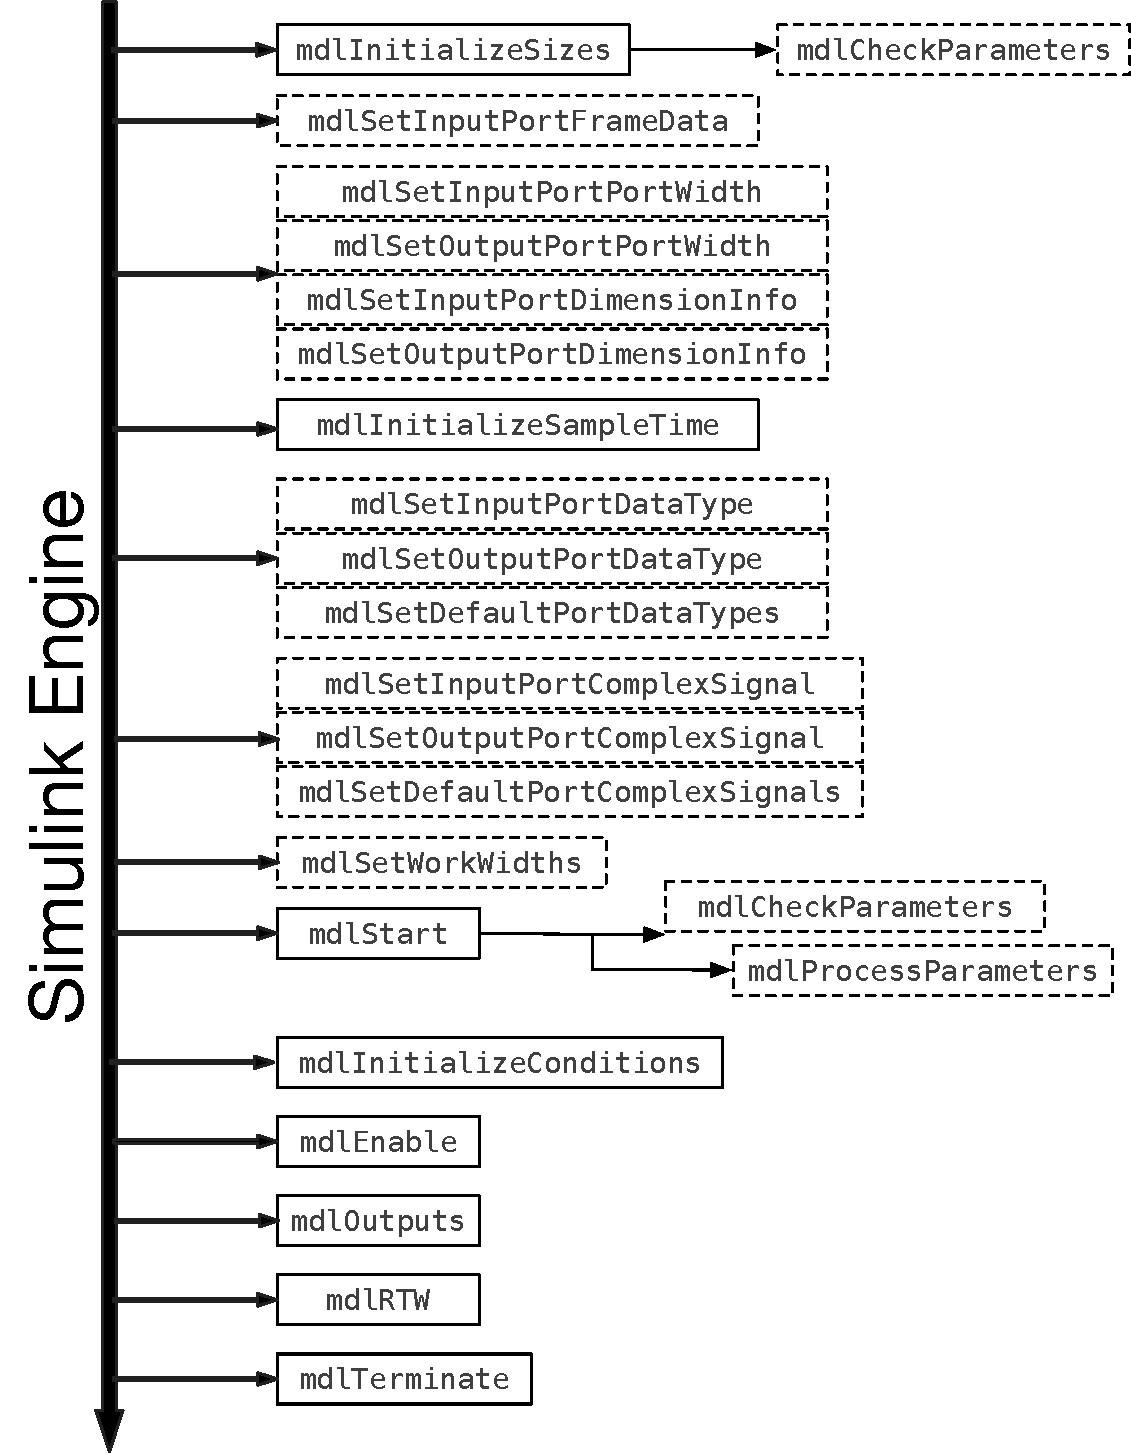
\includegraphics[width=0.8\textwidth]{RTWCallbacks}
\caption{Simulink Engine Callbacks Order in Case of Code Generation}
\label{fig:RTWCallbacks}
\end{figure}
The function \verb|mdlInitializeSizes| is important because it sets the sizes of the various signals and vectors and so can inherit the port configuration information such as the size and the data type. Then through the function \verb|mdlRTW| these parameters are written into the .rtw file to be used by the TLC file.
\par Each block has a target file that determines what code should be generated for that block \cite{BlockTLC}. Within each block target file, \emph{block functions} specify the code to be output during the start function, output function, update function, and so on. After the Code generation block initialization (i.e. \verb|BlockInstanceSetup| and \verb|BlockTypeSetup|) different TLC function generate executable code, let focus on \verb|Start| and \verb|Outputs| which are used for implementing the ports. 
\begin{itemize}
\item \emph{Start}. The code inside this function executes once and only once, therefore, it is used to instantiate a global variable for the port descriptor and to initialize it (i.e. open the port).
\item \emph{Output}. The code inside this function is placed in model's Outputs function and generate the code required to access the port.
\end{itemize}

%********************************** % Section  **************************************
\section{System Target File}\label{slexSTF}
Once the model has been adapted to the software architecture described in the configuration file, a Matlab script file scans the model start the code generation process. The script run the command \verb|rtwbuild| on every subsystem, so RTW creates a folder in the current working directory and places all the generated files. In order to drive the code generation process a \emph{custom System Target File} has been developed.% \ref{sec:RTWGenerationProcess} 
\par The custom System Target File generate C code as the default System Target File from Embedded Coder would do (see section \ref{sec:CodeArchitecture}). This is achieved by exploiting the built-in TLC script \verb|codegenentry.tlc|. The generation process is incremental, so every time a new block is encountered, some code is added to the temporary data structure that later on will be combined to form the source files. At the end of the process, when all the information about the code is known, an additional XML file is generated. The file describes the interface of the generated code, including:
\begin{itemize}
\item \emph{BuildDir}. The sub-folder of the current working directory where the source files are stored.
\item \emph{SrcFiles}. The list of all the source files.
\item \emph{Header and Body}. The header and the body of the subsystem, this are the main file implementing the subsystem code.
\item \emph{Inputs and Outputs}. The name of the structure containing the Inputs/Outputs for the subsystem code and every structure element (ports) with its name and dimension.
\item \emph{Functions}. The name of the entry point functions.
\end{itemize}
An example of a subsystem called \verb|Ctrl1Err| is the following:
\lstinputlisting{Chapters/SrcCode/Ctrl1Err.xml}
This file is required because every generation process ignores all the others, particularly, the last one, which should glue all the code to form PikeOS processes and partitions, does not know anything about the code interface of the subsystems. An alternative to the XML format might be an RTW file. The drawback of this approach is that now also the Partitions generation must be done through a TLC file and Matlab, whereas, with an XML file there is a free choice about the code generation tool. Moreover, via XML file is easier to implement a heterogeneous code generation tool.

\paragraph{} Even though any other code generation tool can be used, the Partition generation is implemented used a TLC file for seamless integration with the current workflow.

%********************************** % Section  **************************************
\section{Native Application Generation}
For generating the code of each PikeOS Process (one for each Partition), another template is required. It must take the previously generated code and transform in threads than pack them in Processes. This task is performed by another TLC script.
\par The process is driven by a Matlab script that parses every XML file that has been generated by the custom System Target File enriching them with the information stored in the configuration file. The result of this operation is the previously created class structure with additional information, i.e.:
\begin{itemize}
\item Threads
\begin{itemize}
\item Code interfaces
\item Communications
\item Affinity Mask
\item Priority
\item Partition Identifier
\end{itemize}
\item Partitions
\end{itemize}
The top level class provides a public method to export all the threads inside a given partition as RTW file. This method is useful to feed the TLC script.

\subsection{PikeOS Process Generation}\label{nativeprocess}
Every PikeOS Partition is made by the Main thread and several child threads. The main thread is loaded by the PikeOS kernel, and it is responsible for initializing all the children threads. Therefore, to implement the proposed software architecture, the main thread perform the following operations:
\begin{enumerate}
\item Lower its priority to the lowest in its partition to let child threads execute their initialization code.
\item Creates all the child threads.
\item Increase its priority to the highest in its partition.
\item Enter in an infinite loop where resume all child threads and wait for the next period activation.
\end{enumerate}
The C code implementing this behavior in PikeOS is the following:
\lstinputlisting[language=C]{Chapters/SrcCode/SimpleMain.c}
Where \verb|<AffinityMask>|, \verb|<Name>| and \verb|<Prototype>| are variable that change for each thread, like in TLC script. The functions \verb|initThread| and \verb|resumeThread| are custom functions. The first one creates a PikeOS thread and sets its affinity mask, the second one resume a thread from the STOPPED state.
\par When the main lower its priority to the lowest one, the scheduler ensures that every child thread executes its initialization code than the main execute again and elevates its priority. During normal operation, the main is the highest priority thread in the partition and resumes all the threads, therefore the scheduler ensures that no one of the child thread executes before the main has resumed all threads, so the correct behavior is satisfied.

\paragraph{} The child threads have a similar structure. Every thread:
\begin{enumerate}
\item Once created, execute the initialize function of the subsystems it refers to.
\item Move to the STOPPED state, waiting for the first activation.
\item Enters into an infinite loop where. Take all the require output from the predecessors, execute the step function of the subsystem it refers to and goes again in the STOPPED state, waiting for the next activation.
\end{enumerate}
The C code implementing this behavior is the following:
\lstinputlisting[language=C]{Chapters/SrcCode/SimpleThread.c}
As discussed before, all the threads inside a process share the same virtual memory space, so an output variable for a subsystems is a global variable that can be freely retrieved by one of it successor. This communication, referred as \emph{inter-partition communication}, might require synchronization while accessing shared resources.

\subsection{Intra-Process Communication}
Assuming a non-preemptive, FIFO priority-based scheduler and a correct priority assignment, there is no need to use any synchronization mechanism when two threads on the same core try to access a shared variable. This because the scheduler ensures that the thread with the lower priority (the reader) does not execute before the completion of the higher priority thread (the writer). When the access occurs between threads scheduled on different cores there is no guarantee about the read-write operation. There might be cases in which a reader tries to get the input variable before its predecessor wrote the last value. In this case, a synchronization mechanism must be placed to avoid it.

\subsubsection{Spinlocks}
Several synchronization mechanisms solve the inter-core communication issue, the most commonly used locks are \emph{mutexes} and \emph{semaphores}.% that keep track of the number of times it has been locked and so manage thread access when it is unlocked. 
 Both mechanisms eventually block the caller thread by moving it to the WAITING state, meaning that the next schedulable thread in the queue becomes the CURRENT thread and execute. Suppose that thread $\tau_1$ perform a lock on a mutex and moves to the WAITING state, then a thread $\tau_2$ from the READY queue is scheduled. Might happen that there is a precedence relation $\tau_1\to\tau_2$ that force $\tau_2$ to block, waiting for $\tau_1$ to complete. This can happen again with the next scheduled thread and so on. Therefore, this might lead to a sequence of threads first check if all the predecessors completed their execution and eventually blocks.
\par A mechanism that avoids this drawback is the \emph{spinlock} (already described in section \ref{sec:spinlocks}). With this mechanism the thread performs a busy-wait (basically loops) on the lock until it is unlocked, so does not move to the WAITING state. Therefore, whenever the spinlock is released, the thread is sure about the availability of all the predecessor data. This mechanism, which is very cost-effective when the thread is expected to wait for a small amount of time, does not introduce the preemption issue.
\par Therefore, the TLC script adds a call to \verb|p4_spin_lock| on every read and a \verb|p4_spin_unlock| on every write on shared variables that needs to be accessed by threads scheduled on different cores.

%********************************** % Section  **************************************
\section{Operating System Configuration Generation}
As discussed in the section \ref{sec:IntegrationProject}, the Integration Project provide a way to configure the generation of the PikeOS boot image, including all the Partitions. The Integration Project uses the file \verb|project.xml| to store all the configuration information. The generation of the whole file is complex, so, for the seek of simplicity only some XML snippets are generated. This does not lead to a loss of functionality because it is possible to develop a tool that, once an Integration Project has been generated by CODEO or the command line, can scan the \verb|project.xml| File and add programmatically the snippets. 
\par The snippets that are required are the following:
\begin{itemize}
\item Partition and Ports
\item Channels
\item Schedule Scheme
\end{itemize}
With a procedure analogue to the generation of the partitions, the workspace structure containing all the information is exported in the RTW File format and used by a TLC to generate these snippets.

\subsection{Partitions and Ports}
First and foremost Resource Partitions and and their Processes musts be defined. This is made by adding some \verb|ComponentInstance| elements as child of the \verb|ConfigurationDomainTable| tag. An example of the definition of a Resource Partition is the following:
\lstinputlisting{Chapters/SrcCode/Snippets/GroupSnippet.xml}
In this snippet all relevant information are defined, i.e. \begin{enumerate*}
\item the partition and its name (e.g. PartitionA),
\item the process belonging to this partition (e.g. ProcessA),
\item the ports and their identifier (e.g.\verb|sport_0_src|).
\end{enumerate*} In this example both the Process and the Partition are grouped in a group called \verb|Partition A| (which has no impact on the boot image creation) but it is displayed in the CODEO Project Configuration.

\paragraph{} Later on in the \verb|project.xml| File, the complete enumeration of the Resource Partitions is listed as child elements of \verb|PartitionTable|, a configuration example is:
\lstinputlisting{Chapters/SrcCode/Snippets/PartitionsSnippet.xml}
Here are defined two Resource Partitions, \verb|PartitionA| and \verb|PartitionB|.

\subsection{Channels}
Once Resource Partition and their Ports are declared, Channels must connect them allowing two Partition to communicate. For example a communication between partition $\pi_2$ and partition $\pi_3$ through ports \verb|sport_0_dst| (end point of the communication) and \verb|sport_0_src| (starting point of the communication) is the following:
\lstinputlisting{Chapters/SrcCode/Snippets/ChannelsSnippet.xml}
The \verb|Channel| tag, with its children, is a child of the tag \verb|PartitionChannelTable| in the \verb|ConnetctionTable|.

\subsection{Schedule Scheme}
The schedule scheme is used to implement the Partition Schedule. As discussed in section \ref{sec:P4Scheduler}, a Schedule Scheme is by Time Windows, each of them has an identifier, a starting time and a duration. The default scheme loaded by the kernel is called \verb|SCHED_BOOT|. An example of the schedule snippet is the following.
\lstinputlisting{Chapters/SrcCode/Snippets/ScheduleSnippet.xml}
In this schedule the remaining time after the schedule of \TP{1} and \TP{2} and before the start of a new Major Time Frame (Hyper-period) is allocated to the \TP{0}. The flag \verb|VM_SCF_PERIOD| mark that time window as the start of a new period. This flag is used by PikeOS kernel to notify the Main threads to wake up.
%!TEX root = ../thesis.tex

\chapter{Test and Validation}

\ifpdf
    \graphicspath{{Chapters/Figs/Raster/}{Chapters/Figs/PDF/}{Chapters/Figs/}}
\else
    \graphicspath{{Chapters/Figs/Vector/}{Chapters/Figs/}}
\fi

%********************************** % Intro *****************************************
%Il framework che è stato sviluppato (\ref{sec:DevelopedFramework}) prevede 3 fasi, lo sviluppo del modello, lo scheduling e la generazione di codice. Per dimostrare il funzionamento del framework viene presentato un esempio.

%********************************** % Section  **************************************
\section{Example model}
The example from the EMC2 project not relatively straightforward for showing the tool capabilities. Therefore, as test example model, let consider a quad-rotor flight control with a pan/tilt camera on it shown in figure \ref{fig:exampleModel}. The pan and tilt camera is moved by two servo motors controlled by two PID that do not communicate with the flight control of the drone. The adopted drone control scheme is taken from \cite{PeterCorke2011} with minor changes introduced to comply with our design restrictions. The original model in \cite{PeterCorke2011} contains different functional loops, each of them has been included in a Simulink subsystem representing a task. The quad-rotor and the motors dynamics that has been used during the simulation have been substituted to enable code generation. The \emph{Quadrotor} block contains the control for its motors and the interface to its sensors. The motors blocks are interface blocks to their encoders. The pan/tilt motor control has a sample time of $0.05$ seconds, the drone flight control a sample time of $0.1$ seconds and the quad-rotor block a sample time of $0.01$ seconds.
\begin{figure}[htbp] 
\centering    
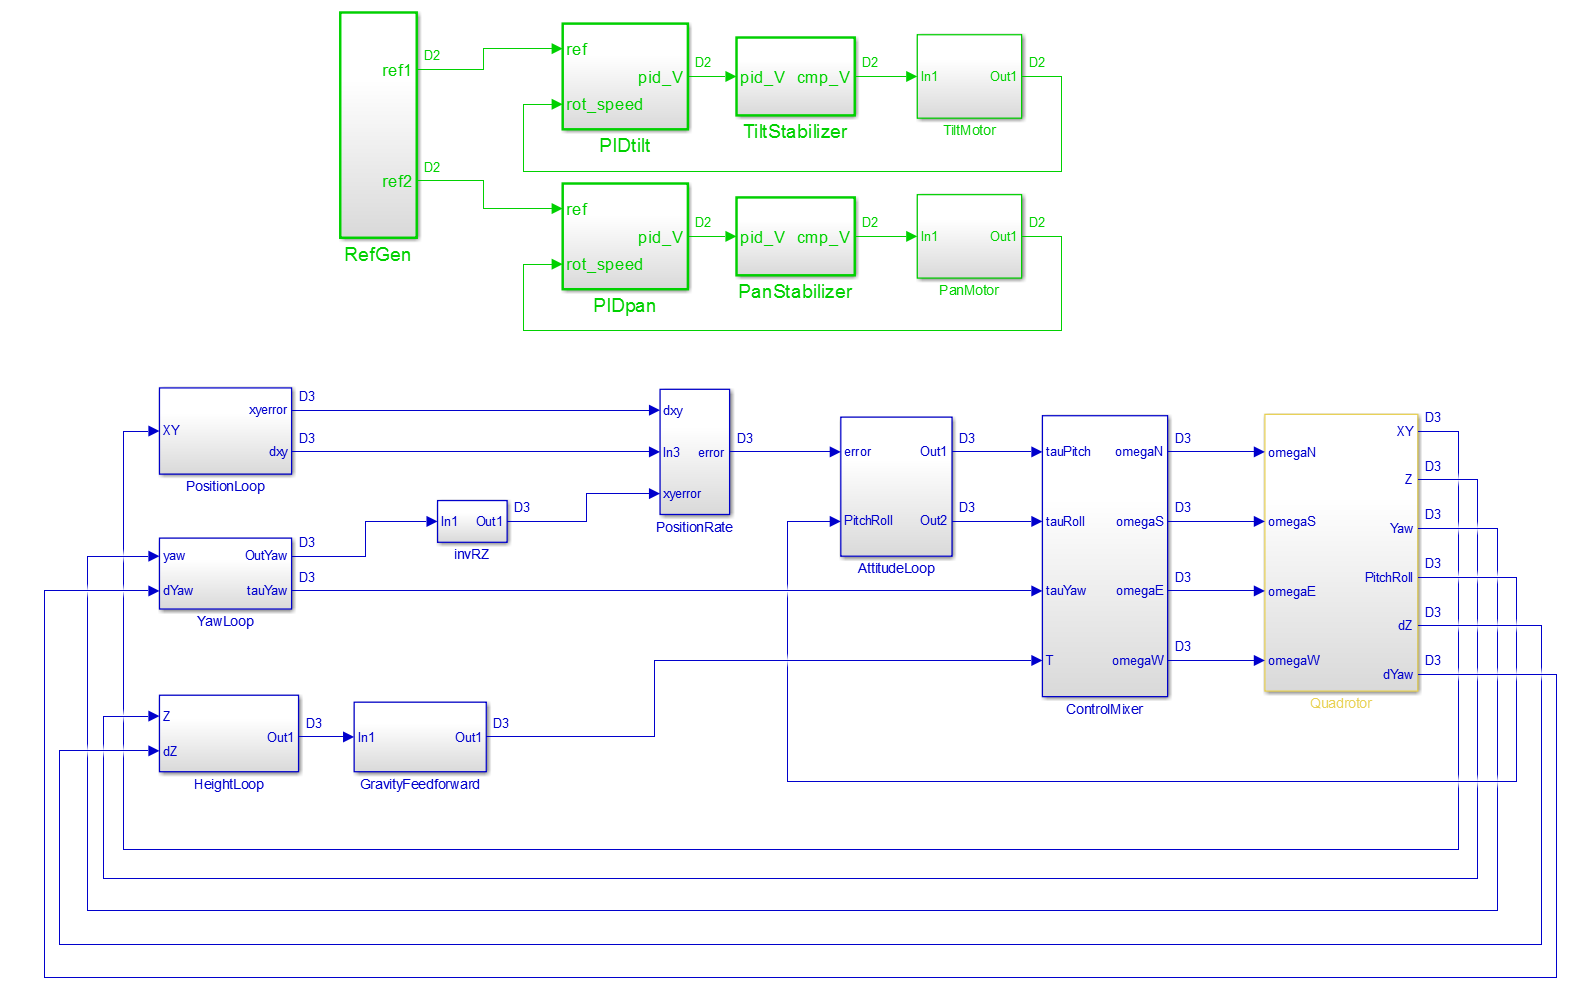
\includegraphics[width=0.9\textwidth]{CompiledModel}
\caption{Example Model}
\label{fig:exampleModel}
\end{figure}

This example is oriented to demonstrate the capabilities of the framework, so it does not focus on the performance of the controller. When the model is ready to be used, the framework GUI (fig. \ref{fig:GUI}) can be started with the command \verb|START|. 
\begin{figure}[htbp] 
\centering    
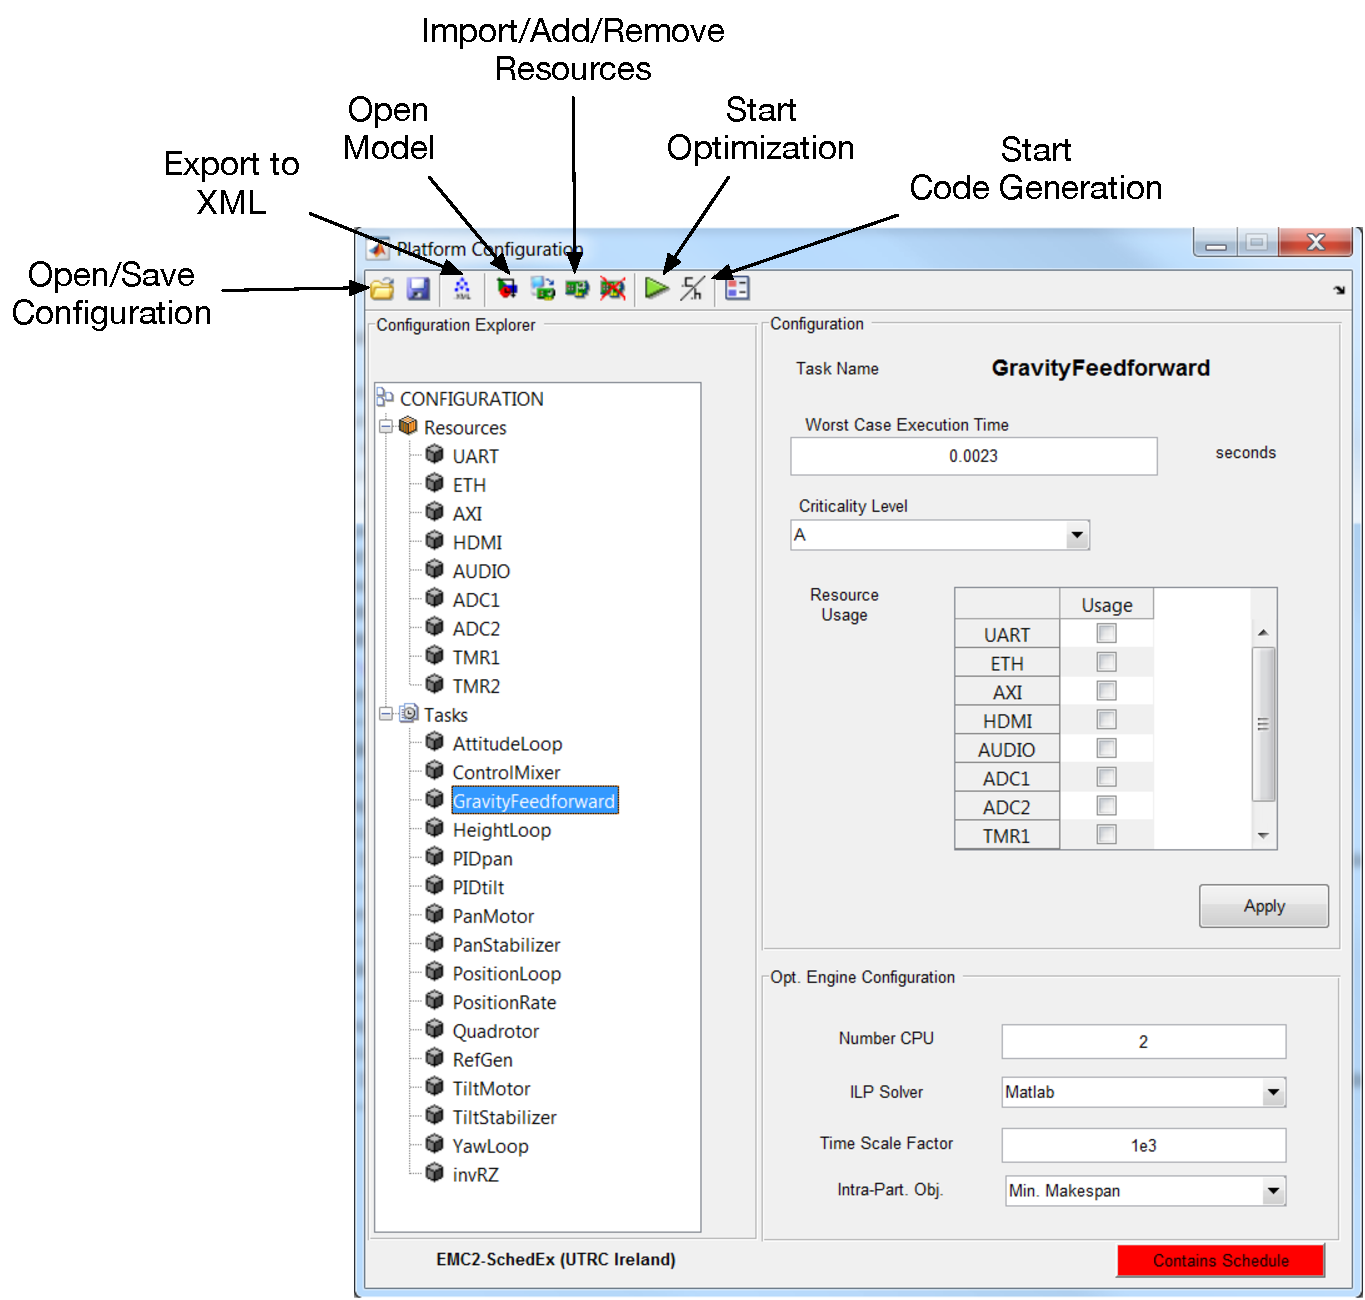
\includegraphics[width=0.6\textwidth]{PlatformConfiguration}
\caption{Tool Graphic User Interface (GUI)}
\label{fig:GUI}
\end{figure}
Here the designer can configure all the additional parameters that are required for each task. In particular, he can add all the resources on the platform, set up the optimization engine and specify for each task:
\begin{enumerate}
\item The Worst-Case Execution Time
\item The Criticality level (A to E)
\item The Resources the task uses
\end{enumerate}
In our example, the tasks are configured as shown in table \ref{tab:taskset}. The WCETs are randomly selected to make the task-set schedulable, otherwise, the inter-partition optimization problem states that no feasible solution is available.
\begin{table}
\begin{center}
\begin{tabular}{llcccc}  
\toprule
Task ID & Task Name    & Period & WCET & Criticality & Resources \\
\midrule
1  & AttitudeLoop      	& $0.1$  &	$9.135\cdot10^{-4}$     & A	& --\\
2  & ControlMixer     	& $0.1$  & 	$9.8412\cdot10^{-4}$    & A	& --\\
3  & GravityFeedforward & $0.1$  & 	$8.7592\cdot10^{-4}$    & A	& AXI \\
4  & HeightLoop      	& $0.1$  & 	$0.0012$			    & A	& AXI \\
5  & PIDpan      		& $0.05$ & 	$9.7148\cdot10^{-4}$    & B	& --\\
6  & PIDtilt      		& $0.05$ & 	$8.5084\cdot10^{-4}$    & B	& --\\
7  & PanMotor      		& $0.05$ & 	$5.4351\cdot10^{-4}$    & B	& AXI, ADC1\\
8  & PanStabilizer     	& $0.05$ &	$5.6589\cdot10^{-4}$    & B	& --\\
9  & PositionLoop      	& $0.1$  & 	$9.9352\cdot10^{-4}$    & A	& UART \\
10 & PositionRate      	& $0.1$  & 	$5.9584\cdot10^{-4}$    & A	& --\\
11 & Quadrotor      	& $0.01$ & 	$0.0033$			    & A	& AXI \\
12 & RefGen      		& $0.05$ & 	$4.8490\cdot10^{-4}$    & B	& UART \\
13 & TiltMotor      	& $0.05$ &	$4.0925\cdot10^{-4}$    & B	& AXI, ADC2\\
14 & TiltStabilizer     & $0.05$ & 	$9.0944\cdot10^{-4}$    & B	& --\\
15 & YawLoop      		& $0.1$  &	$8.2928\cdot10^{-4}$    & A	& --\\
16 & invRZ      		& $0.1$  &	$9.5648\cdot10^{-4}$    & A	& --\\
\bottomrule
\end{tabular}
\caption {Example Model Task-set}
\label{tab:taskset}
\end{center}
\end{table}
The task-set will be allocated on a dual-core processor and scheduled minimizing the makespan.

\subsection{Feedthrough relationships}
To fully understand the resulting functional model it is important to highlight the feedthrough relationship among ports of each subsystem. In figure \ref{fig:feedthrough} are shown all the paths. 
\begin{figure}[htbp] 
\centering    
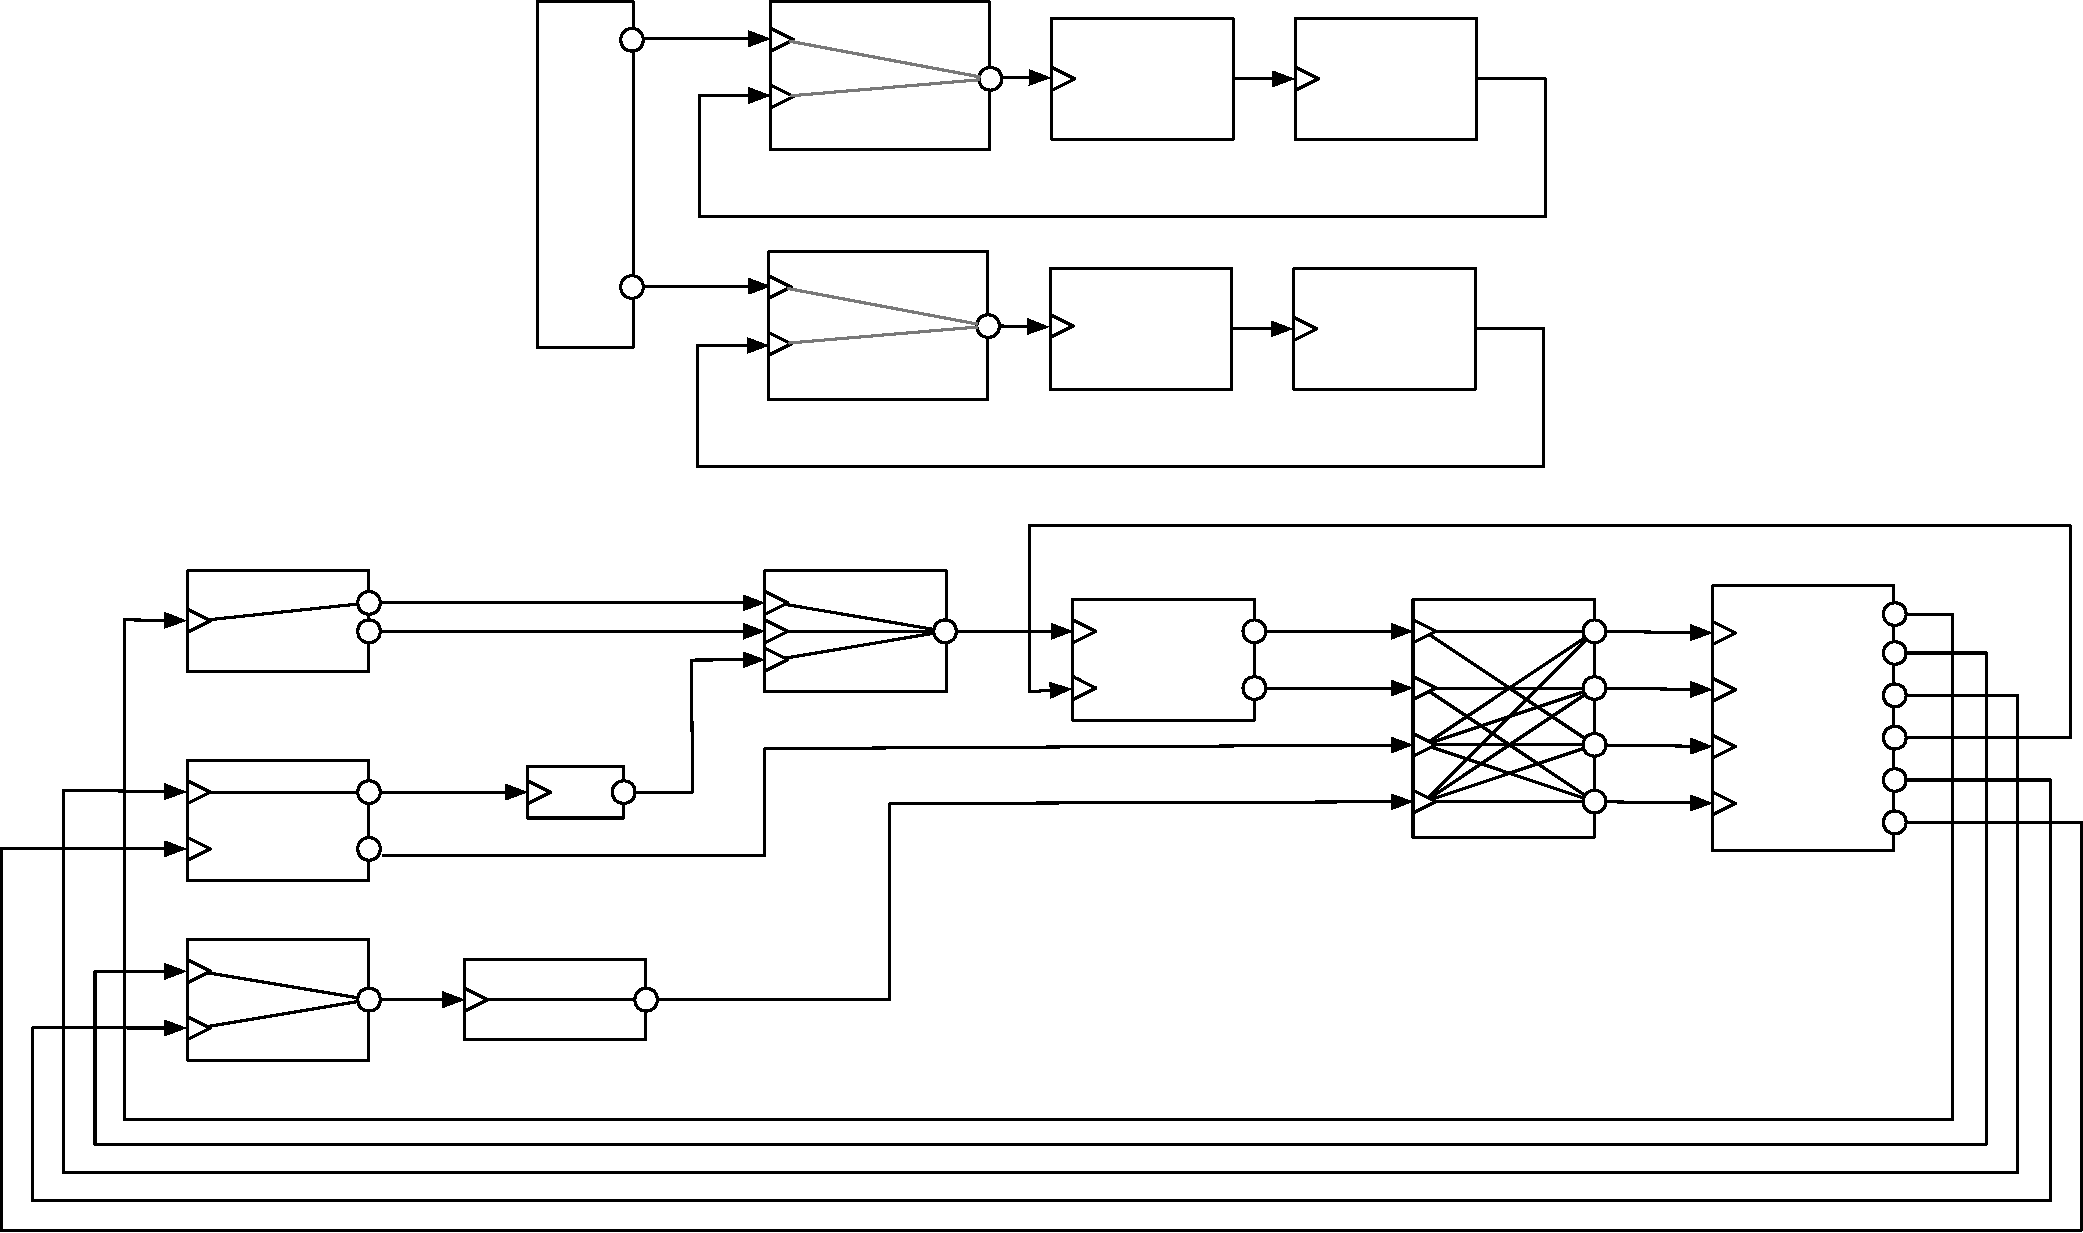
\includegraphics[width=0.7\textwidth]{FeedRelationships}
\caption{Feedthrough Relationships}
\label{fig:feedthrough}
\end{figure}
This relationship is automatically extracted from the model by a Matlab script and used to build the functional model.

%********************************** % Section  **************************************
\section{Functional Model Extraction}
Once the configuration is complete (i.e. WCET, Resources and Criticality), the system designer can start the scheduling process. The first step is the DAG extraction, which is transparent to the designer. Indeed, it is extracted  as soon as the GUI (or the model) is opened. The Direct-Acyclic Graph representing the task-set is shown in figure \ref{fig:extaskset}.
\begin{figure}[htbp] 
\centering    
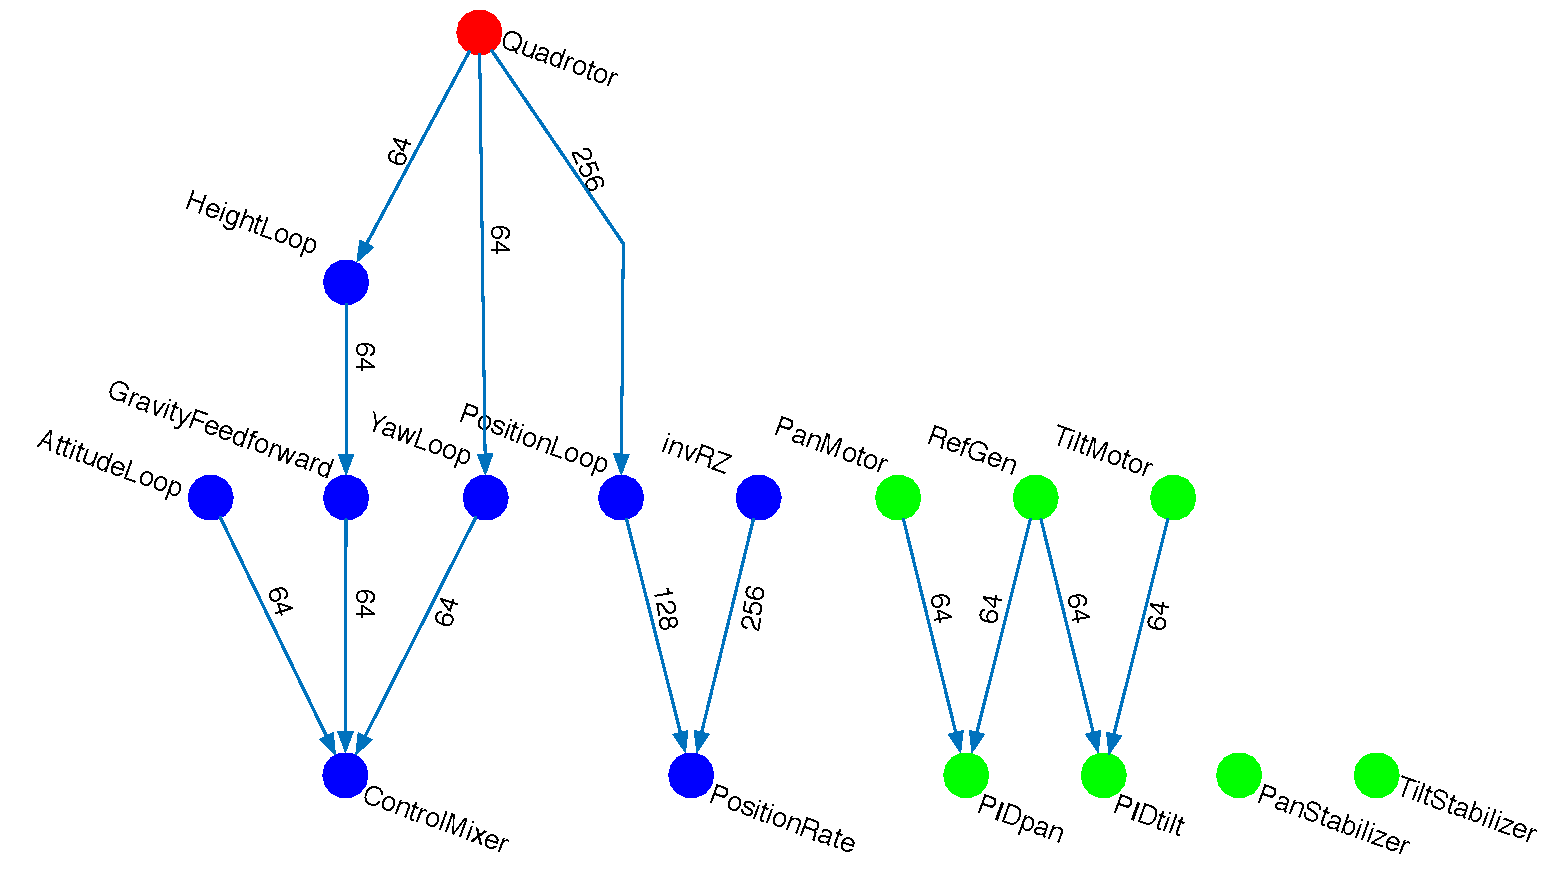
\includegraphics[width=0.9\textwidth]{Taskset}
\caption{Example Functional model - Task-set}
\label{fig:extaskset}
\end{figure}
Each color represent a different sample time, the edges the dependency among tasks. From the Simulink model, all the lines connecting two blocks where the input port of the destination block is not in a feedtrough relationship, has disappeared. This is the representation of the model used by the partitioning and scheduling algorithm.

%********************************** % Section  **************************************
\section{Scheduling}
The DAG, enriched with the information manually configured by the designer is the main input for the partitioning and scheduling algorithm. As already explained in section \ref{sec:DevelopedFramework}, the scheduling process is made by three phases: \begin{enumerate}
\item Partitioning
\item Intra-Partition Scheduling
\item Inter-Partition Scheduling
\end{enumerate}


\subsection{Partitioning}
The partitioning algorithm implements some form of robust partitioning of the task-set graph, the result of this step is figure \ref{fig:pdag} and is called P-DAG. While grouping tasks in partitions, some edge in the task-set cut the boundary of the partition, this edge represents a dependency among two partitions.
\begin{figure}[htbp] 
\centering    
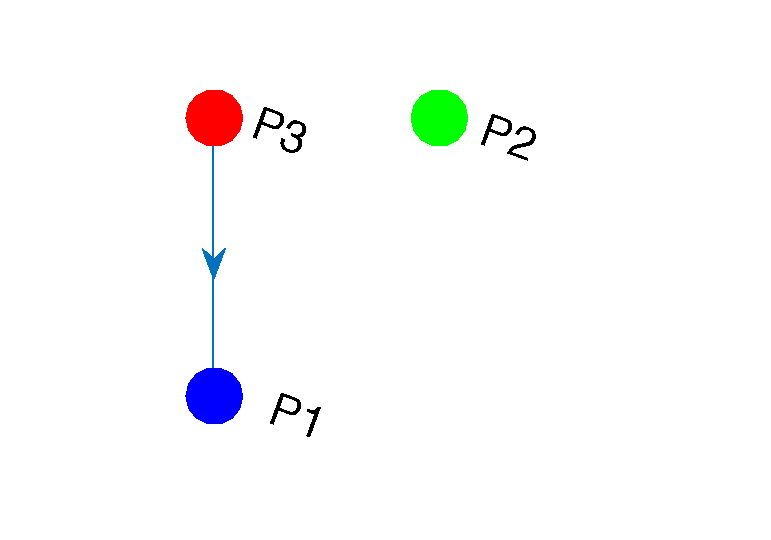
\includegraphics[width=0.3\textwidth]{PDAG}
\caption{Partition Graph, P-DAG}
\label{fig:pdag}
\end{figure}
All the edges in the P-DAG represent the partial order of execution imposed by the flow preservation requirement. The how tasks are redistributed in partitions is shown in table \ref{tab:partitions}.
\begin{table}
\begin{center}
\begin{tabular}{llc}  
\toprule
Partition & Tasks & Period \\
\midrule
P1  & 1,2,10,16,3,4,9,15 & $0.1$\\
P2  & 5,6,7,8,12,13,14 & $0.05$\\
P3  & 11 & 0.01\\
\bottomrule
\end{tabular}
\caption {Partitions}
\label{tab:partitions}
\end{center}
\end{table}

% \begin{figure}
%   \begin{subfigure}{1\textwidth}
%     \centering
%     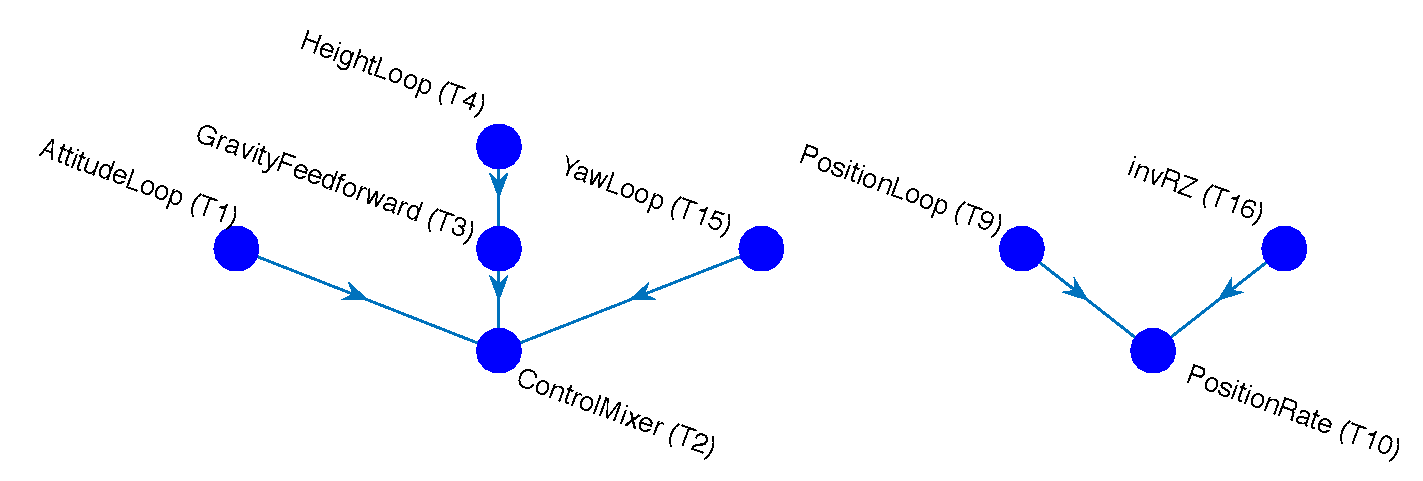
\includegraphics[width=1.0\textwidth]{TDAG1}
%     \caption{T-DAG Partition 1}
%     \label{fig:tdag1}
%   \end{subfigure}
%   \begin{subfigure}{1\textwidth}
%     \centering
%     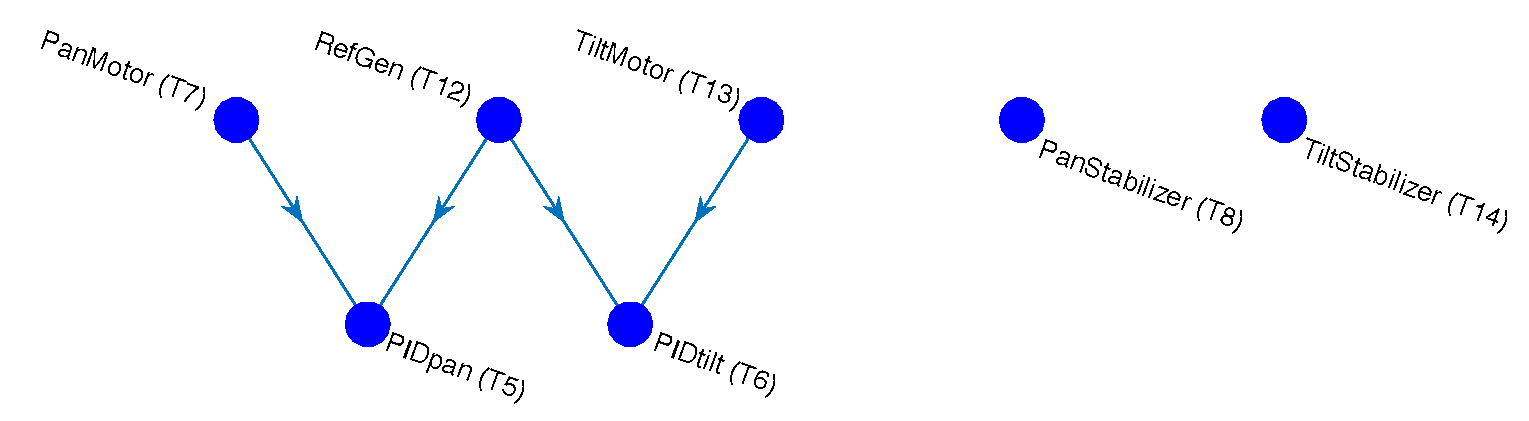
\includegraphics[width=1.0\textwidth]{TDAG2}
%     \caption{T-DAG Partition 2}
%     \label{fig:tdag2}
%   \end{subfigure}
%   \begin{subfigure}{1\textwidth}
%   \centering
%     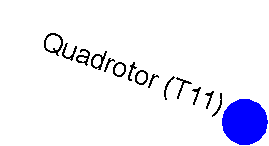
\includegraphics[width=0.2\textwidth]{TDAG3}
%     \caption{T-DAG Partition 3}
%     \label{fig:tdag3}
%   \end{subfigure}
%   \caption{T-DAGs}
%   \label{fig:tdag}
% \end{figure}

\subsection{Intra-Partition Scheduling}
Each node of the P-DAG represent a partition so, each partition contains some tasks, the subgraph of the task-set graph related to a partition is called T-DAG. % (figure \ref{fig:tdag}).
The allocation and scheduling of each T-DAG is called \emph{Intra-Partition Scheduling}. For each T-DAG the MILP optimization problem is solved on the relative subgraph (table \ref{tab:milp}). Note that task three and four cannot execute in parallel in partition one because both use the AXI interface (resource). Similarly, task 7 and 13 cannot execute in parallel in partition 2. This constraint is encoded in the incompatibility matrix.
\begin{table}
\begin{center}
\begin{tabular}{cccc}  
\toprule
Partition & Solution Time & Number of Constraints & Number of Variables (continuous) \\
\midrule
P1  & 0.34 seconds & 313 & 161(16)\\
P2  & 0.09 seconds & 237 & 127(14)\\
P3  & 0.03 seconds & 3 	 & 6(2)\\
\bottomrule
\end{tabular}
\caption {MILP formulations}
\label{tab:milp}
\end{center}
\end{table}
The resulting schedule is depicted in figure \ref{fig:intra}.

\begin{figure}
  \begin{subfigure}{0.8\textwidth}
    \centering
    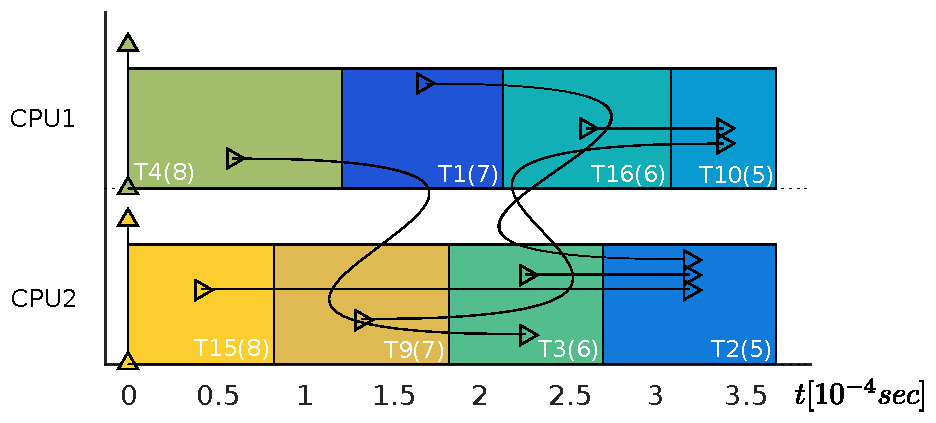
\includegraphics[width=1.0\textwidth]{intraP1}
    \caption{Partition 1 Schedule}
    \label{fig:intraP1}
  \end{subfigure}
  \begin{subfigure}{0.8\textwidth}
    \centering
    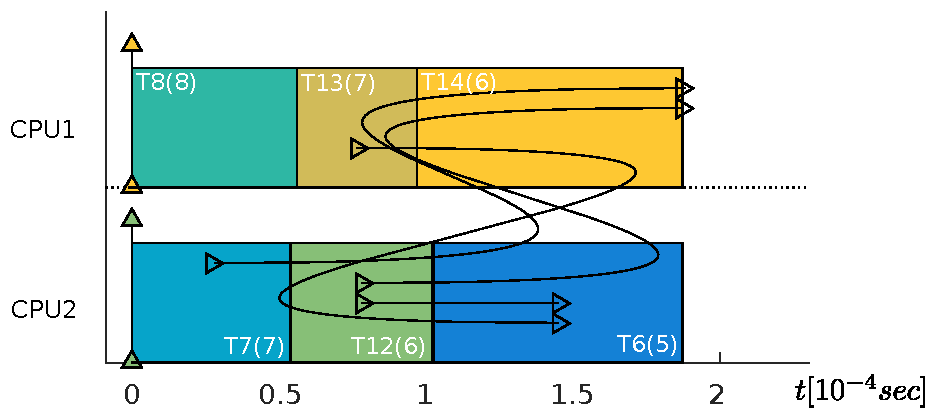
\includegraphics[width=1.0\textwidth]{intraP2}
    \caption{Partition 2 Schedule}
    \label{fig:intraP2}
  \end{subfigure}
  \begin{subfigure}{0.8\textwidth}
  \centering
    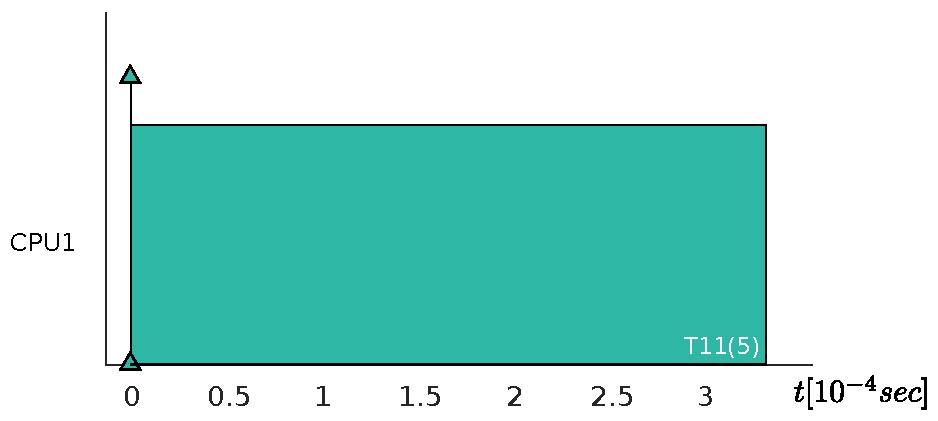
\includegraphics[width=1.0\textwidth]{intraP3}
    \caption{Partition 3 Schedule}
    \label{fig:intraP3}
  \end{subfigure}
  \caption{Intra-Partition Schedule}
  \label{fig:intra}
\end{figure}

Again, the arrows among tasks represent the dependency relationship.

%PARTITION 1
% V 	= [1,		2,			10,		16,			3,			4,	  9,			15]
% CPU 	= 1     	2     		1     	1     		2     		1     2     		2
% Start = 0.0012    0.0027    0.0031    0.0021    0.0018         0    0.0008         0
%PARTITION 2
% V 	= [5,		6,				7,		8,		12,		13,			14]
% CPU 	=  1     	2     			2		 1     2     	1     		1
% Start = 0.0019    0.0010         0         0    0.0005    0.0006    0.0010
%PARTITION 3
% V 	= 11
% CPU 	=  1
% Start = 0

\subsection{Priority Assignment}
When a schedule is obtained another optimization problem assigns priorities to each task as described in section \ref{sec:priorityassignment}. In particular figure \ref{fig:PriorityAssignment} shows that some priority value can be left unused for allowing some low priority task to be executed, in this example we use an offset of 5 for solving the optimization problem. The resulting assignment is shown in figure \ref{fig:intra}, tasks priorities are enclosed by parenthesis.
%	  [1,    2,    10,  16,	   3,    4,    9,    15]
%P1 => 7     5     5     6     6     8     7     8
%     [5,    6,    7,    8,    12,   13,   14]
%P2 => 5     5     7     8     6     7     6
%P3 => 5

\subsection{Inter-Partition Scheduling}
The final step of the scheduling process is the inter-partition scheduling. As described in section \ref{interpartition}, the Bratley algorithm is exploited to find the optimal solution. To include precedence constraints and periodicity, the P-DAG must be factorized. In the current example the Hyper-period is $0.1$ seconds, so, inside this interval partition $P_1$ execute only one, partition $P_2$ execute twice and partition $P_3$ execute 10 times. The resulting factorized P-DAG is shown in figure \ref{fig:fPDAG}.
\begin{figure}[htbp] 
\centering    
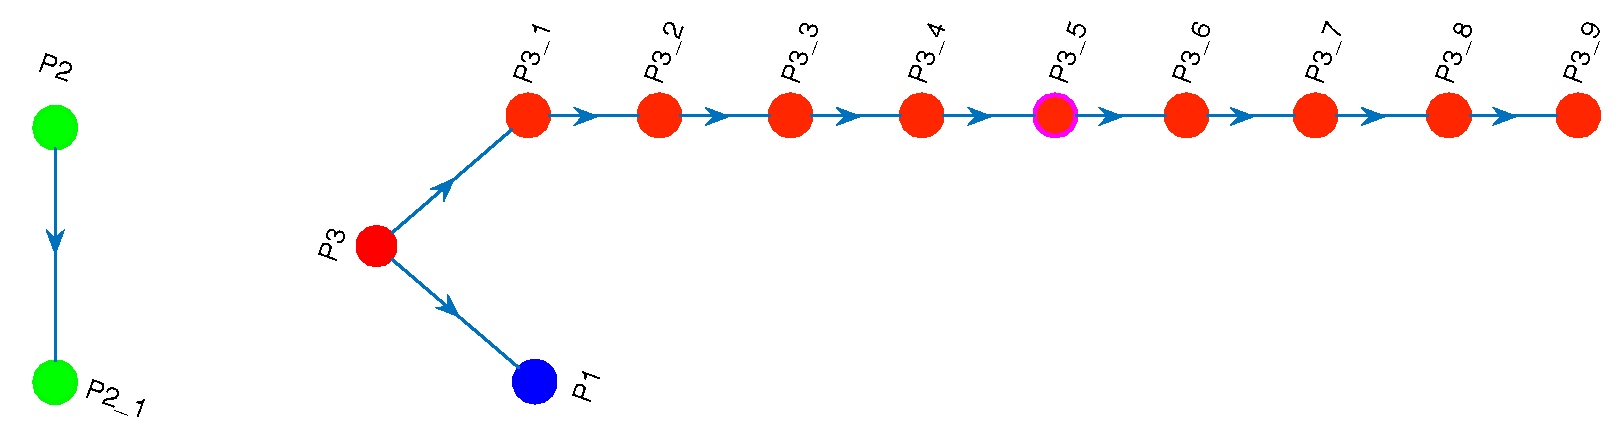
\includegraphics[width=0.8\textwidth]{fPDAG}
\caption{Factorized Partition Graph}
\label{fig:fPDAG}
\end{figure}

Thanks to Lemma \label{eq:precedenceLemma}, has been proven that if release times and deadlines are consistent with the precedence relation, then any normal one-processor schedule that satisfies the release times and deadlines must also obey the precedence relation, so a release time and a due date can be assigned to each partition according to formula \ref{eq:precedence}. They are summarized in table \label{tab:partitionset}.

\begin{table}
\begin{center}
\begin{tabular}{lcccc}  
\toprule
Partition ID & WCET &  Release Time & Due Date & Activation \\
\midrule
$P_1$ & 0.0037 & 0.0033 & 0.1 &0.0052\\
$P_2$ & 0.0019 & 0 & 0.05 & 0\\
$P_3$ & 0.033 & 0 & 0.01 & 0.0019\\
$P_2^1$ & 0.0019 & 0.05 & 0.01 & 0.05\\
$P_3^1$ & 0.033 & 0.01 & 0.02 & 0.01\\
$P_3^2$ & 0.033 & 0.02 & 0.03 & 0.02\\
$P_3^3$ & 0.033 & 0.03 & 0.04 & 0.03\\
$P_3^4$ & 0.033 & 0.04 & 0.05 & 0.04\\
$P_3^5$ & 0.033 & 0.05 & 0.06 & 0.0519\\
$P_3^6$ & 0.033 & 0.06 & 0.07 & 0.06\\ 
$P_3^7$ & 0.033 & 0.07 & 0.08 & 0.07\\
$P_3^8$ & 0.033 & 0.08 & 0.09 & 0.08\\ 
$P_3^9$ & 0.033 & 0.09 & 0.11 & 0.09\\
\bottomrule
\end{tabular}
\caption {Partition-set}
\label{tab:partitionset}
\end{center}
\end{table}

The Partition-set in table \ref{tab:partitionset} (except the last column) feeds the Bratley algorithm that enumerate all the possible feasible solution and select the optimal one. Int inter-partition schedule is shown in figure \ref{fig:inter}. All the activation times for each partition is listed in table \ref{tab:partitionset} (last column).
\begin{figure}[htbp] 
\centering    
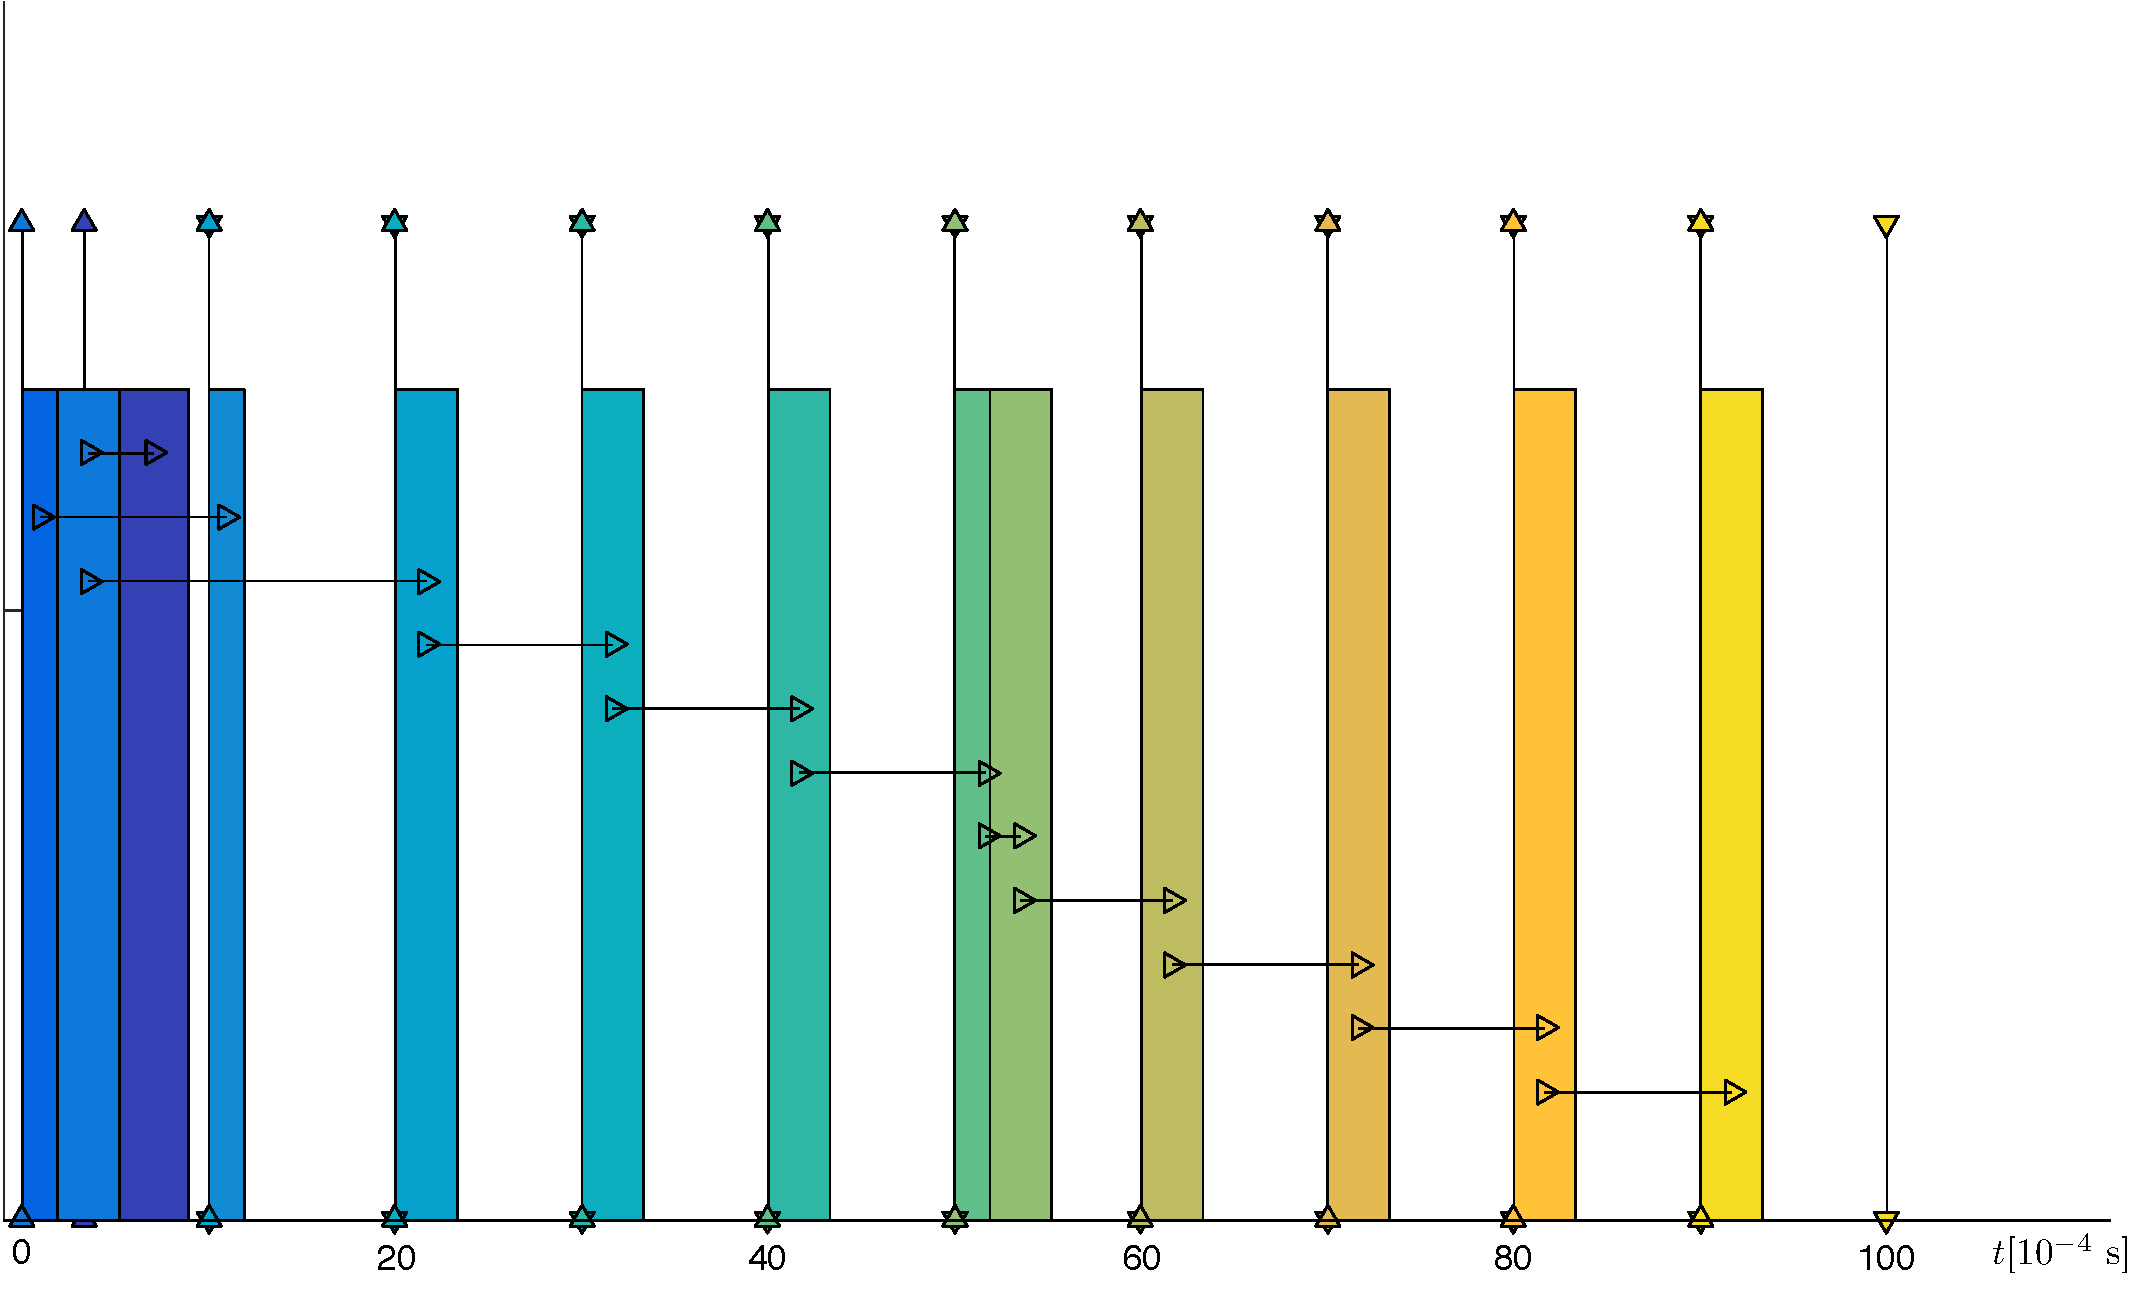
\includegraphics[width=0.8\textwidth]{inter}
\caption{Inter-Partition Schedule}
\label{fig:inter}
\end{figure}

\subsection{Theoretical Performance}
In order to assert how well the model can be run on multi-core, various metrics need to be defined first. Using the right metric makes it possible to determine how one would benefit from parallelizing the model as well as how various actions like changing the model changed the performance. In this work only widely used performance metrics for parallel systems are used, since a system’s performance is the main motivation behind switching to a multi-core architecture. These include the makespan (mentioned in the previous section), the \emph{speed-up} and the \emph{efficiency} \cite{grama2003}.

\paragraph{} When used for parallel systems, the makespan can be divided into two metrics: \emph{sequential makespan} and \emph{parallelized makespan}. The sequential makespan is the execution time required by the task-set to execute on a single-core. Used together with the parallelized makespan, which is the execution time on multiple cores, various other metrics like the speed-up can be calculated. 
\par Speed-up is defined as the ratio of the elapsed time when executing a program on a single processor (the sequential makespan $W_1$) to the execution time when $p$ processors are available (the parallelized makespan $W_p$)\cite{speedup}. Throughout this work, it is defined as,
\begin{equation}
    S(p) = \frac{W_1}{W_p}
\end{equation}
With this metric it is possible to assert how the execution time of a system as improved by changing the number of cores. In theory, the speed-up can never exceed the number of processors $p$, the best case. This introduces the \emph{efficiency}. It is defined as the average utilization of the $p$ allocated processors \cite{speedup}. This value tells us how much average speedup is gained by investing in $p$-core, enabling us to declare how worthwhile a multi-core system is for a given system. Formally it is defined as:
\begin{equation}
    E(p)=\frac{S(p)}{p}
\end{equation}
Efficiency can only reach values between 0 and 1. Programs with linear speed-up have an efficiency of 1. It is worth mentioning that in practice, linear speed-up is not achievable in practice since adding more processors increases the communication time between processors as well as the time waiting for shared resources to unlock, which are not considered in this model.

\paragraph{} For each partition both the speed-up and the efficiency can be computed, they are summarized in table \ref{tab:performance}.
\begin{table}
\begin{center}
\begin{tabular}{lcccc}  
\toprule
Partition & Speed-up & Efficiency \\
\midrule
$P_1$ & 1.9927 & 0.99\\
$P_2$ & 1.9927 & 0.99\\
$P_3$ & 1 & 0.5\\
\bottomrule
\end{tabular}
\caption {Performance}
\label{tab:performance}
\end{center}
\end{table}
The MILP problem, since finds the optimal solution, does a good job in exploiting all the possible time in the partition on both available cores. There is no idle time in the intra-partition schedule (see fig. \ref{fig:intra}) so the speed-up is approximately 2 for partition one and partition two.

\paragraph{} At this point all the information about the scheduling are known, so the code generation process can be started.

%********************************** % Section  **************************************
\section{Code Generation}
Once a feasible schedule is available, the system designer can start the code generation process pressing the button \emph{Start Code Generation} in the framework GUI. This operation will save the current schedule to an XML file and call the code generation entry point. After parsing the file, the model is adapted to the communication model described in the exported configuration.

\subsection{Adapted model}
As described in section \ref{sec:modelAdapt}, before generating the C code, all the subsystem ports that are communication data to subsystem assigned to another partition needs to be substituted with the correct operation on a Sampling Port. This is automatically done by the script after parsing the configuration file. In figure \ref{fig:adaptedModel} it is possible to see that all the lines connecting \verb|Quadrotor| with all other blocks disappeared. As expected, all partitions are isolated one from each other, meaning that there are no lines between blocks.
\begin{figure}[htbp] 
\centering    
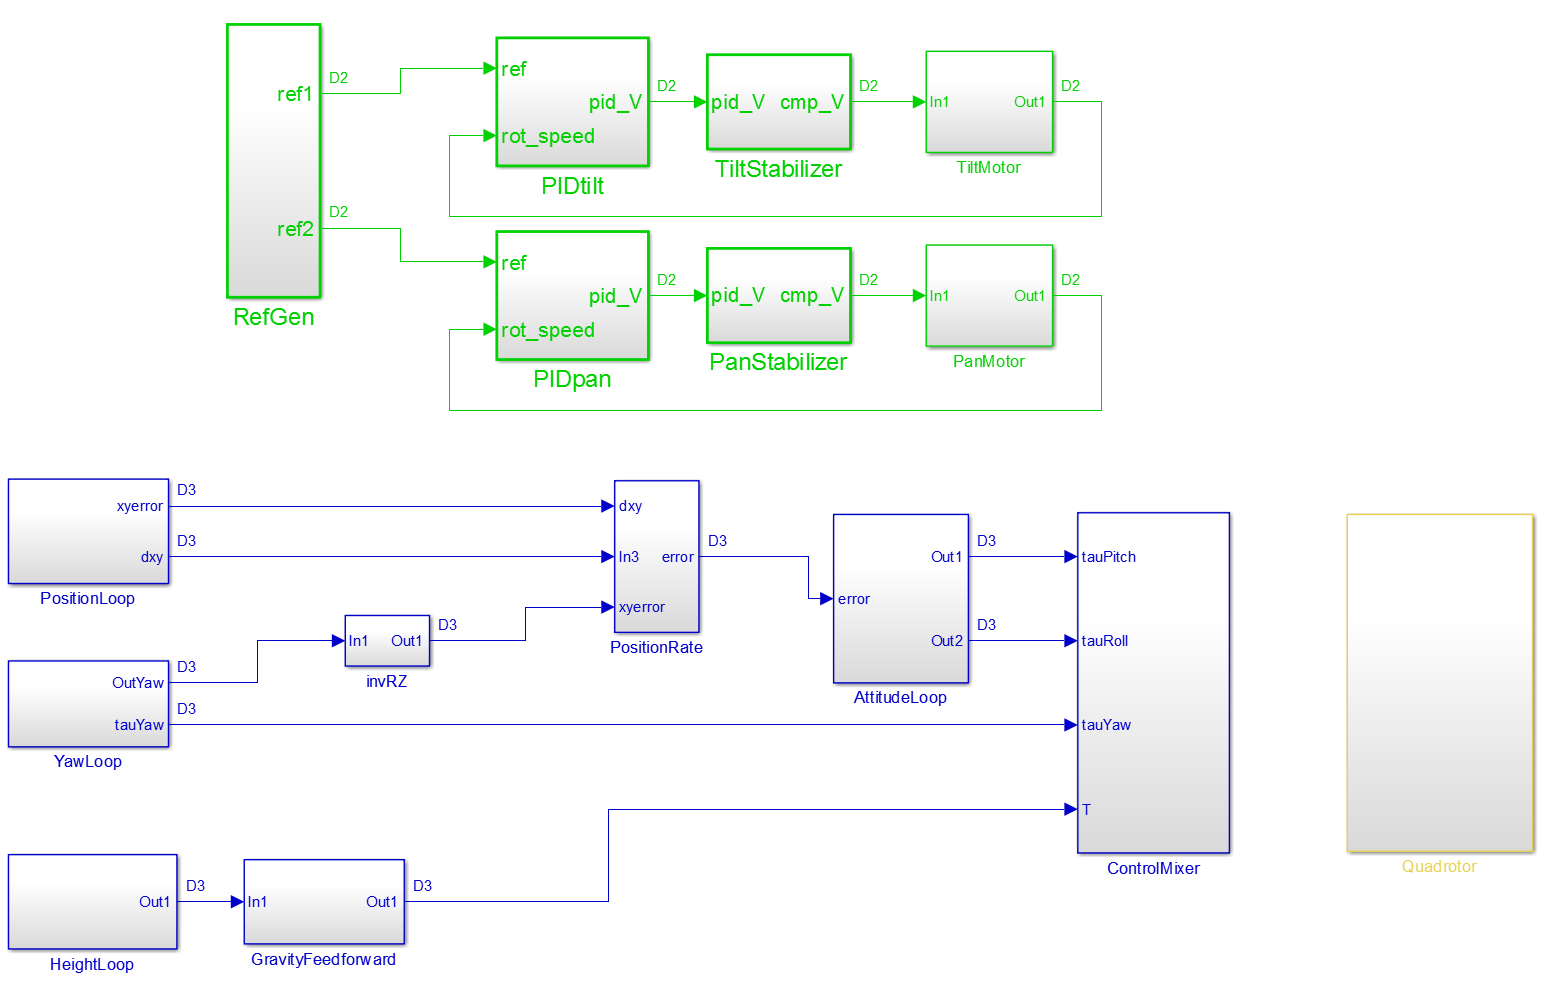
\includegraphics[width=1\textwidth]{AdaptedModel}
\caption{Adapted Model}
\label{fig:adaptedModel}
\end{figure}
The next step generates the C code for each block.

\subsection{Partition Main Threads}
To generate the code of each block is used the System Target file described in section \ref{slexSTF}. It generates the C code for each single block as Embedded Coder would do, also it generates an XML file describing the structure of the code. When all the blocks have been generated, all these XML files are collected and parsed to correctly generate the code of each partition.

\paragraph{} As described in section \ref{nativeprocess}, each Native PikeOS process is made by the main thread and all the thread composing that partition. The code for this two entities is inside separate files for each partition, e.g. \verb|P1_main.c|, \verb|P2_main.c|, \verb|P3_main.c|. As an example let consider the code of the main thread of partition one.
\lstinputlisting[language=C]{Chapters/SrcCode/P1_main.c}
The threads it creates matches the ones in \ref{tab:partitions} for $P_1$ with the priorities in figure \ref{TBD}. It also initializes some spinlocks, one for each inter-core communications, each of them can be graphically seen in figure \ref{fig:intra} by edges between tasks scheduled on different cores.
\par After creating and letting each thread to execute its initialization code (lines 15-30) the main thread enters an infinite loop where each thread is resumed every time a new period starts.

\paragraph{} As an example let consider the code of the thread about \verb|AttitudeLoop| (thread 1), this is interesting because is used both data directly from a thread in the same process and data coming from the sampling port. The code of this thread is the following.
\begin{lstlisting}[language=C]
static void AttitudeLoop_thread(void){
      P4_e_t rc;

      AttitudeLoop_initialize();
      vm_cprintf("AttitudeLoop initialized...\n");
      p4_thread_stop(P4_THREAD_MYSELF);

      /* Continous loop */
	for(;;){
		/* Input update */
		AttitudeLoop_U.pitchrolldmd[0] = PositionRate_Y.error[0];
		AttitudeLoop_U.pitchrolldmd[1] = PositionRate_Y.error[1];

		/* Step */
		AttitudeLoop_step();

		/* Unlock Spinlocks */
		P4_spin_unlock(&AttitudeLoop1_ControlMixer1_spinlock);
		p4_spin_unlock(&AttitudeLoop2_ControlMixer2_spinlock);

		/* Wait for next period */
		p4_thread_stop(P4_THREAD_MYSELF);
	}

	/* Terminate - Never Reached */
	AttitudeLoop_terminate();
}
\end{lstlisting}
On lines 11-12 it takes the data directly from the shared structure. The data from the sampling port are retrieved inside the \verb|AttitudeLoop_step()| because the code for reading from the port is generated directly from RTW thanks to the Custom Block. Indeed, inside the file \verb|AttitudeLoop.c|, the following code appears.
\begin{lstlisting}[language=C]
P4_e_t rc1 = vm_sport_read(&AttitudeLoop_sport1_d, &AttitudeLoop_B.PitchRoll[0],
    4*sizeof(real_T), &read_size, &validity);
\end{lstlisting}
When the step function of the subsystem has been executed, the successor that is executing on another core can be notified. For this reason, two spinlocks are unlocked on lines 18-19 notifying the thread \verb|ControlMixer| that the data are available. Finally, the thread goes in the STOPPED state on line 22, waiting for the next activation from the main thread.

\subsection{Integration Project Snippets}
Out of the code generation process, some XML snippets are generated to help the configuration of the Integration Project. For the sake of conciseness, they are nor reported here because they are quite long. For example, schedule scheme is 64 lines long since in every moment there is at least one partition active, this means that for each gap in the schedule of figure \ref{fig:inter} the \TP{0} is statically allocated for non-real time operation (e.g. muxa and other services).


%!TEX root = ../thesis.tex

\chapter{Conclusions}

\ifpdf
    \graphicspath{{Chapters/Figs/Raster/}{Chapters/Figs/PDF/}{Chapters/Figs/}}
\else
    \graphicspath{{Chapters/Figs/Vector/}{Chapters/Figs/}}
\fi


%********************************** % Section  **************************************
\section{Contributions}
%Goals: Studiare l'applicazione di hypervisors per mix-critical applications. Usare il Model-Based Design approach per superare la complessita' di implementare applicazioni safe & secure. 
%è stato sviluppato un framework personalizzabile per la generazione di codice per sistemi multicore ARINC-xxx compliant. Sfrutta le potezialità (ormai mature) di RTW ma senza usare il concurrent workflow (che invece non è maturo). è stato sviluppato un framework  per la schedulazione di sistemi mix-critical anche se non  è sufficiente a gestire correntamente applicazioni mix-critical è un punto di partenza.

Multi-core platforms have been introduced in many different settings, but so far they have not been utilized in the domain of safety-critical avionic real-time systems. A substantial amount of work has been put into the evaluation of hypervisors to address the security and safety for such applications.
\par In this thesis, the area of code generation for mixed-critical application in multi-core embedded systems is taken into account. For this purpose, a Model-Based design framework, supported by Simulink, has been developed. It is a proof-of-concept integrated tool that allows the designer to design and deploy hard real-time, mixed-critical applications with the assistance of optimization problems and code generation.

%********************************** % Section  **************************************
\section{Future works}

\paragraph{} The planned future work has two separate tracks. One is related to the optimization framework and aims at extending it with support for more comprehensive, robust partitioning algorithm. The second track of future work relates to the code generation process.

\subsection{Scheduling and allocation}
A current limitation of this work is that the validity of the proposed design framework has been extensively tested in simulation, but no experimental validation was conducted. Extensive testing and robustness improvements are needed to improve the effectiveness of the partitioning and scheduling framework. Improvements on the partitioning algorithm are necessary to improve safety and security of the implemented code. One step ahead in this direction might find some heuristics that estimates the impact of one step to the others. Another approach might be trying to encode each phase into a single MILP optimization problem. A possible drawback of the second method is that it can lead to problems which complexity makes them barely solvable for a small task-set. 
\par A possible improvement for the scheduling algorithm might be to analyze more in depth how cache and memory interferences and delays can be minimized by the partitioning or the scheduling. An additional step might be added, in the current implementation there is a one-to-one map between subsystems and tasks, there can be cases in which this is not the optimal choice.

\paragraph{} Another current limitation of the current implementation it the needs of the system designer to specify the Worst-Case Execution Time of each task. 
\par Worst Case Execution Time analyses aim at determining an upper bound for a task execution time. Usually, the result of a WCET analysis is an upper approximation of the exact WCET which is nearly impossible to determine for real life Software. Simple architectures allow WCET determination using static analysis techniques using a model of execution. That means that the analyzed software is not executed but compiled and analyzed. On complex COTS processors architectures, it is not possible to determine an accurate model. Today, an alternative method is used. A worst case scenario is defined from an analysis performed on the Airborne Software. The execution time is measured under this scenario and is further corrected with parameters taking into account variability during operations. Timing analysis is tough in multi-core COTS due to the lack of information on the processor behavior. It may lead to a pessimistic estimation of those parameters. 
\par There are a plenty of free and commercial tool for the timing analysis, some of them are directly integrated into the Simulink environment. These tools can be used to alleviate the workload of the system designer that can focus more on the architecture optimization. 
However, there is a lack of research on WCET estimation under faulty conditions on safety-critical, multi-core COTS platforms that require temporal partitioning. This research is needed to deploy multi-core platforms in the avionics domain safely and for certification authorities to accept and approve their usage.

\paragraph{} Another path to explore is the area of formal verification instead of empirical measurement-based methods. Formal methods with temporal specifications can be used to prove that a given set of partitions, with their tasks, can never reach hazardous states. This proof would be another great help for certification authorities.

\subsection{Code Generation}
The biggest limitation of the current code generator is that it does not support non-periodic tasks. This is not an intrinsic limitation of the approach, instead, it has not been implemented yet. All the non-periodic tasks can be placed on PikeOS \TP{0} thanks to the gaps left in the priority assignment. At the moment has not been implemented a semantics to mark those tasks.

\paragraph{} An interesting improvements might be the support for the Hardware-in-the-Loop (HIL) Simulation. HIL simulation, which is quite common in the Aviation industry, is a type of real-time simulation, it can be used to test the controller design. In HIL simulations, the real controller responds to realistic stimuli coming from the virtual plant included in the model. HIL simulation can add great value to WCET estimation.

\paragraph{} Another possible improvement might be improving the resource usage in the generated code. For example, if a block is sending data to another block via two different ports, and these are converted into sampling ports due to the partitioned architecture, it can be useful to merge the two data into the same port.

\paragraph{} Moreover, the work-flow can be extended to other code generators, and eventually to hand-coded applications. The step in this direction is to model the system in \emph{SysML} \cite{sysml} which is a general-purpose modeling language for engineering systems (defined as an extension of UML) and to use a more generic code generator, such as Acceleo \cite{Acceleo}, to generate the glue code.


% ********************************** Back Matter *******************************
% Backmatter should be commented out, if you are using appendices after References
%\backmatter

% ********************************** Bibliography ******************************
\begin{spacing}{0.9}

% To use the conventional natbib style referencing
% Bibliography style previews: http://nodonn.tipido.net/bibstyle.php
% Reference styles: http://sites.stat.psu.edu/~surajit/present/bib.htm

\bibliographystyle{alpha}
%\bibliographystyle{unsrt} % Use for unsorted references  
%\bibliographystyle{plainnat} % use this to have URLs listed in References
\cleardoublepage
\bibliography{References/references} % Path to your References.bib file


% If you would like to use BibLaTeX for your references, pass `custombib' as
% an option in the document class. The location of 'reference.bib' should be
% specified in the preamble.tex file in the custombib section.
% Comment out the lines related to natbib above and uncomment the following line.

%\printbibliography[heading=bibintoc, title={References}]


\end{spacing}

% ********************************** Appendices ********************************

\begin{appendices}

%%!TEX root = ../thesis.tex
% ******************************* Thesis Appendix A ****************************
\chapter{How to install \LaTeX} 

\section*{Windows OS}

\subsection*{TeXLive package - full version}
\begin{enumerate}
\item	Download the TeXLive ISO (2.2GB) from\\
\href{https://www.tug.org/texlive/}{https://www.tug.org/texlive/}
\item	Download WinCDEmu (if you don't have a virtual drive) from \\
\href{http://wincdemu.sysprogs.org/download/}
{http://wincdemu.sysprogs.org/download/}
\item	To install Windows CD Emulator follow the instructions at\\
\href{http://wincdemu.sysprogs.org/tutorials/install/}
{http://wincdemu.sysprogs.org/tutorials/install/}
\item	Right click the iso and mount it using the WinCDEmu as shown in \\
\href{http://wincdemu.sysprogs.org/tutorials/mount/}{
http://wincdemu.sysprogs.org/tutorials/mount/}
\item	Open your virtual drive and run setup.pl
\end{enumerate}

or

\subsection*{Basic MikTeX - \TeX~ distribution}
\begin{enumerate}
\item	Download Basic-MiK\TeX (32bit or 64bit) from\\
\href{http://miktex.org/download}{http://miktex.org/download}
\item	Run the installer 
\item	To add a new package go to Start >> All Programs >> MikTex >> Maintenance (Admin) and choose Package Manager
\item	Select or search for packages to install
\end{enumerate}

\subsection*{TexStudio - \TeX~ editor}
\begin{enumerate}
\item	Download TexStudio from\\
\href{http://texstudio.sourceforge.net/\#downloads}
{http://texstudio.sourceforge.net/\#downloads} 
\item	Run the installer
\end{enumerate}

\section*{Mac OS X}
\subsection*{MacTeX - \TeX~ distribution}
\begin{enumerate}
\item	Download the file from\\
\href{https://www.tug.org/mactex/}{https://www.tug.org/mactex/}
\item	Extract and double click to run the installer. It does the entire configuration, sit back and relax.
\end{enumerate}

\subsection*{TexStudio - \TeX~ editor}
\begin{enumerate}
\item	Download TexStudio from\\
\href{http://texstudio.sourceforge.net/\#downloads}
{http://texstudio.sourceforge.net/\#downloads} 
\item	Extract and Start
\end{enumerate}


\section*{Unix/Linux}
\subsection*{TeXLive - \TeX~ distribution}
\subsubsection*{Getting the distribution:}
\begin{enumerate}
\item	TexLive can be downloaded from\\
\href{http://www.tug.org/texlive/acquire-netinstall.html}
{http://www.tug.org/texlive/acquire-netinstall.html}.
\item	TexLive is provided by most operating system you can use (rpm,apt-get or yum) to get TexLive distributions
\end{enumerate}

\subsubsection*{Installation}
\begin{enumerate}
\item	Mount the ISO file in the mnt directory
\begin{verbatim}
mount -t iso9660 -o ro,loop,noauto /your/texlive####.iso /mnt
\end{verbatim}

\item	Install wget on your OS (use rpm, apt-get or yum install)
\item	Run the installer script install-tl.
\begin{verbatim}
	cd /your/download/directory
	./install-tl
\end{verbatim}
\item	Enter command `i' for installation

\item	Post-Installation configuration:\\
\href{http://www.tug.org/texlive/doc/texlive-en/texlive-en.html\#x1-320003.4.1}
{http://www.tug.org/texlive/doc/texlive-en/texlive-en.html\#x1-320003.4.1} 
\item	Set the path for the directory of TexLive binaries in your .bashrc file
\end{enumerate}

\subsubsection*{For 32bit OS}
For Bourne-compatible shells such as bash, and using Intel x86 GNU/Linux and a default directory setup as an example, the file to edit might be \begin{verbatim}
edit $~/.bashrc file and add following lines
PATH=/usr/local/texlive/2011/bin/i386-linux:$PATH; 
export PATH 
MANPATH=/usr/local/texlive/2011/texmf/doc/man:$MANPATH;
export MANPATH 
INFOPATH=/usr/local/texlive/2011/texmf/doc/info:$INFOPATH;
export INFOPATH
\end{verbatim}
\subsubsection*{For 64bit OS}
\begin{verbatim}
edit $~/.bashrc file and add following lines
PATH=/usr/local/texlive/2011/bin/x86_64-linux:$PATH;
export PATH 
MANPATH=/usr/local/texlive/2011/texmf/doc/man:$MANPATH;
export MANPATH 
INFOPATH=/usr/local/texlive/2011/texmf/doc/info:$INFOPATH;
export INFOPATH

\end{verbatim}



%\subsection{Installing directly using Linux packages} 
\subsubsection*{Fedora/RedHat/CentOS:}
\begin{verbatim} 
sudo yum install texlive 
sudo yum install psutils 
\end{verbatim}


\subsubsection*{SUSE:}
\begin{verbatim}
sudo zypper install texlive
\end{verbatim}


\subsubsection*{Debian/Ubuntu:}
\begin{verbatim} 
sudo apt-get install texlive texlive-latex-extra 
sudo apt-get install psutils
\end{verbatim}


\end{appendices}

% *************************************** Index ********************************
\printthesisindex % If index is present

\end{document}
